\chapter{触觉} \label{chap:chap19}

在关于触觉的这一章中,我们将重点放在手上,因为它对这种方式很重要,特别是它在物体特性的欣赏和熟练的运动任务执行中的作用。
人手是进化的伟大创造之一。
我们手指的精细操作能力之所以成为可能,是因为它们具有精细的感觉能力;
如果我们失去了手指的触觉,我们就失去了手的灵巧性。





无毛皮肤的柔软度和顺应性在触觉中起着重要作用。
当物体接触手时,皮肤会顺应其轮廓,形成物体表面的镜像。
由此产生的皮肤位移和压痕会拉伸组织,从而刺激接触区域或接触区域附近的机械感受器的感觉末梢。


当我们用手操纵物体和探索世界时,这些感受器高度敏感并持续活跃。
它们向大脑提供有关物体在手中的位置、形状和表面纹理、施加在接触点的力的大小以及手或物体移动时这些特征如何随时间变化的信息。
指尖是身体中神经支配最密集的部位之一,提供了关于手部操作的物体的广泛而冗余的体感信息。


此外,手的解剖结构及其多个关节和适当的手指使人类能够以反映物体整体形状的方式塑造手,从而提供以手为中心的外部世界本体感受表征。
这种内化物体形状的能力使我们能够创造出可以单独扩展我们双手能力的工具。


当我们熟练使用手术刀或剪刀等工具时,我们会感觉到工具工作表面的状况,就好像我们的手指在那里一样,因为两组触摸感受器监测着这些远程条件下产生的振动和力。
当我们用手指扫过一个表面时,我们会感觉到它的形状和质地,因为另一组机械感受器具有很高的空间和时间敏锐度。
盲人利用这种能力以每分钟一百个单词的速度阅读盲文。 
当我们抓握和操纵一个物体时,我们会非常小心地使用所需的力量,因为特定的机械感受器会持续监控滑动并适当地调整我们的抓握。


我们还能够仅通过触摸来识别放在手中的物体。
当我们拿到棒球时,由于它的形状、大小、重量、密度和质地,我们无需看就能立即认出它。
我们不必考虑每个手指提供的信息就可以推断出该物体一定是棒球;
信息流入记忆并立即匹配先前存储的棒球表示。
即使我们以前从未接触过棒球,我们也会将其视为单个物体,而不是离散特征的集合。
大脑的体感通路有一项艰巨的任务,即整合来自每只手上数千个传感器的信息,并将其转化为适合认知和行动的形式。


为运动控制和认知目的提取感官信息,并为这些目的提取不同种类的信息。
例如,我们可以将注意力从棒球的形状转移到它在手中的位置,以重新调整我们的抓地力以进行有效的投掷或投球。
这种对感觉信息不同方面的选择性关注是由皮层机制引起的。



\section{主动接触和被动触摸有不同的目标}

触摸被定义为两个身体之间的直接接触。
在神经科学中,触觉是指有意识地感知与身体接触的特殊感觉。
触摸可以是主动的,例如当您将手或身体的其他部分移动到另一个表面时;
也可以是被动的,例如当某人或其他东西触摸您时。
% 受试者是意识的一个代理?
\textit{主动接触}从根本上说是一个\textit{自上而下}的过程,在这个过程中,受试者有代理权,寻求特定信息,并控制发生的事情。
主体选择目标的相关显著特征来确定后续行为。
他们选择要抓住的物体和获得它所需的最有效的手形,并决定如何操纵它以实现特定目标。
在主动触摸过程中,体感信息描述了物体的物理特性以及受试者手和手臂的运动,以及它们与任务目标的关系。
重要的是,物体的主动操作是基于触摸的概念,作为一种三维模态,旨在捕捉物体的体积、地形和弹性特性,正如\textit{罗伯塔$\cdot$克莱兹基}和\textit{苏珊$\cdot$莱德曼}首次提出的那样。
这些三维品质最好通过主动操作来领会,包括用手抓握、旋转和轮廓追踪。


被动触摸采用自下而上的过程,在该过程中,受试者对实验者或临床医生指定的外部刺激做出反应。
实验者选择并控制传递到皮肤的刺激的位置、幅度、力、时间、持续时间和空间分布。
随后的行为由范例中提供的指令指导。
触觉刺激分为实验者选择的类别和/或按照密集或快感等级进行评级。
因此,受试者需要分析所有传输的体感信息,并在部分任务说明的指导下选择特定特征。


触觉刺激的主动和被动模式会激发皮肤中相同的受体群,并在传入纤维中引起类似的反应。
它们在反映刺激期间注意力和行为目标的认知特征上有所不同。
通过命名对象或描述感觉来测试被动触觉;
当手操纵物体时使用主动触摸。
触觉的感觉和运动成分在大脑中在解剖学上密切相关,并且在指导运动行为方面具有重要的功能。


在主动触摸过程中,来自大脑皮层运动中枢的下行纤维终止于内侧背角的中间神经元,该中间神经元从皮肤接收触觉信息。
来自皮层运动区的类似纤维终止于背柱核,提供产生行为的运动指令的效应副本(或\textit{伴随发送})(第~\ref{chap:chap30}~章)。
以这种方式,来自手的主动手部运动产生的触觉信号可以集中地与神经学检查或心理物理学测试中被动施加的刺激区分开来。


当患者手部使用有缺陷时,主动和被动触摸之间的区别在临床上很重要。
感觉丧失可能导致无力、僵硬或笨拙等运动缺陷,这就是为什么被动感觉测试在神经系统检查中很重要。
常见的触觉神经学测试包括检测阈值、振动感、两点或纹理辨别力,以及通过触觉识别形状的能力(立体视觉)。 
这些测试测量各种触觉感受器的灵敏度和功能。
与预期值的偏差可能有助于诊断感觉缺陷或导致体感功能障碍的病变。
本章讨论了这些测试背后的神经机制。
其他常见的体感功能测试(腱反射、针刺和热测试)在其他章节中讨论。



\section{手有四种类型的机械感受器}

人手的触觉感觉来自四种机械感受器:\textit{梅斯诺小体}、\textit{梅克尔细胞}、\textit{环层小体}和\textit{鲁菲尼终末器}(图~\ref{fig:19_1})。
每个受体根据其形态、神经支配模式和皮肤深度以独特的方式做出反应。
触觉可以理解为这四个系统协同作用所提供信息的综合结果。


\begin{figure}[htbp]
	\centering
	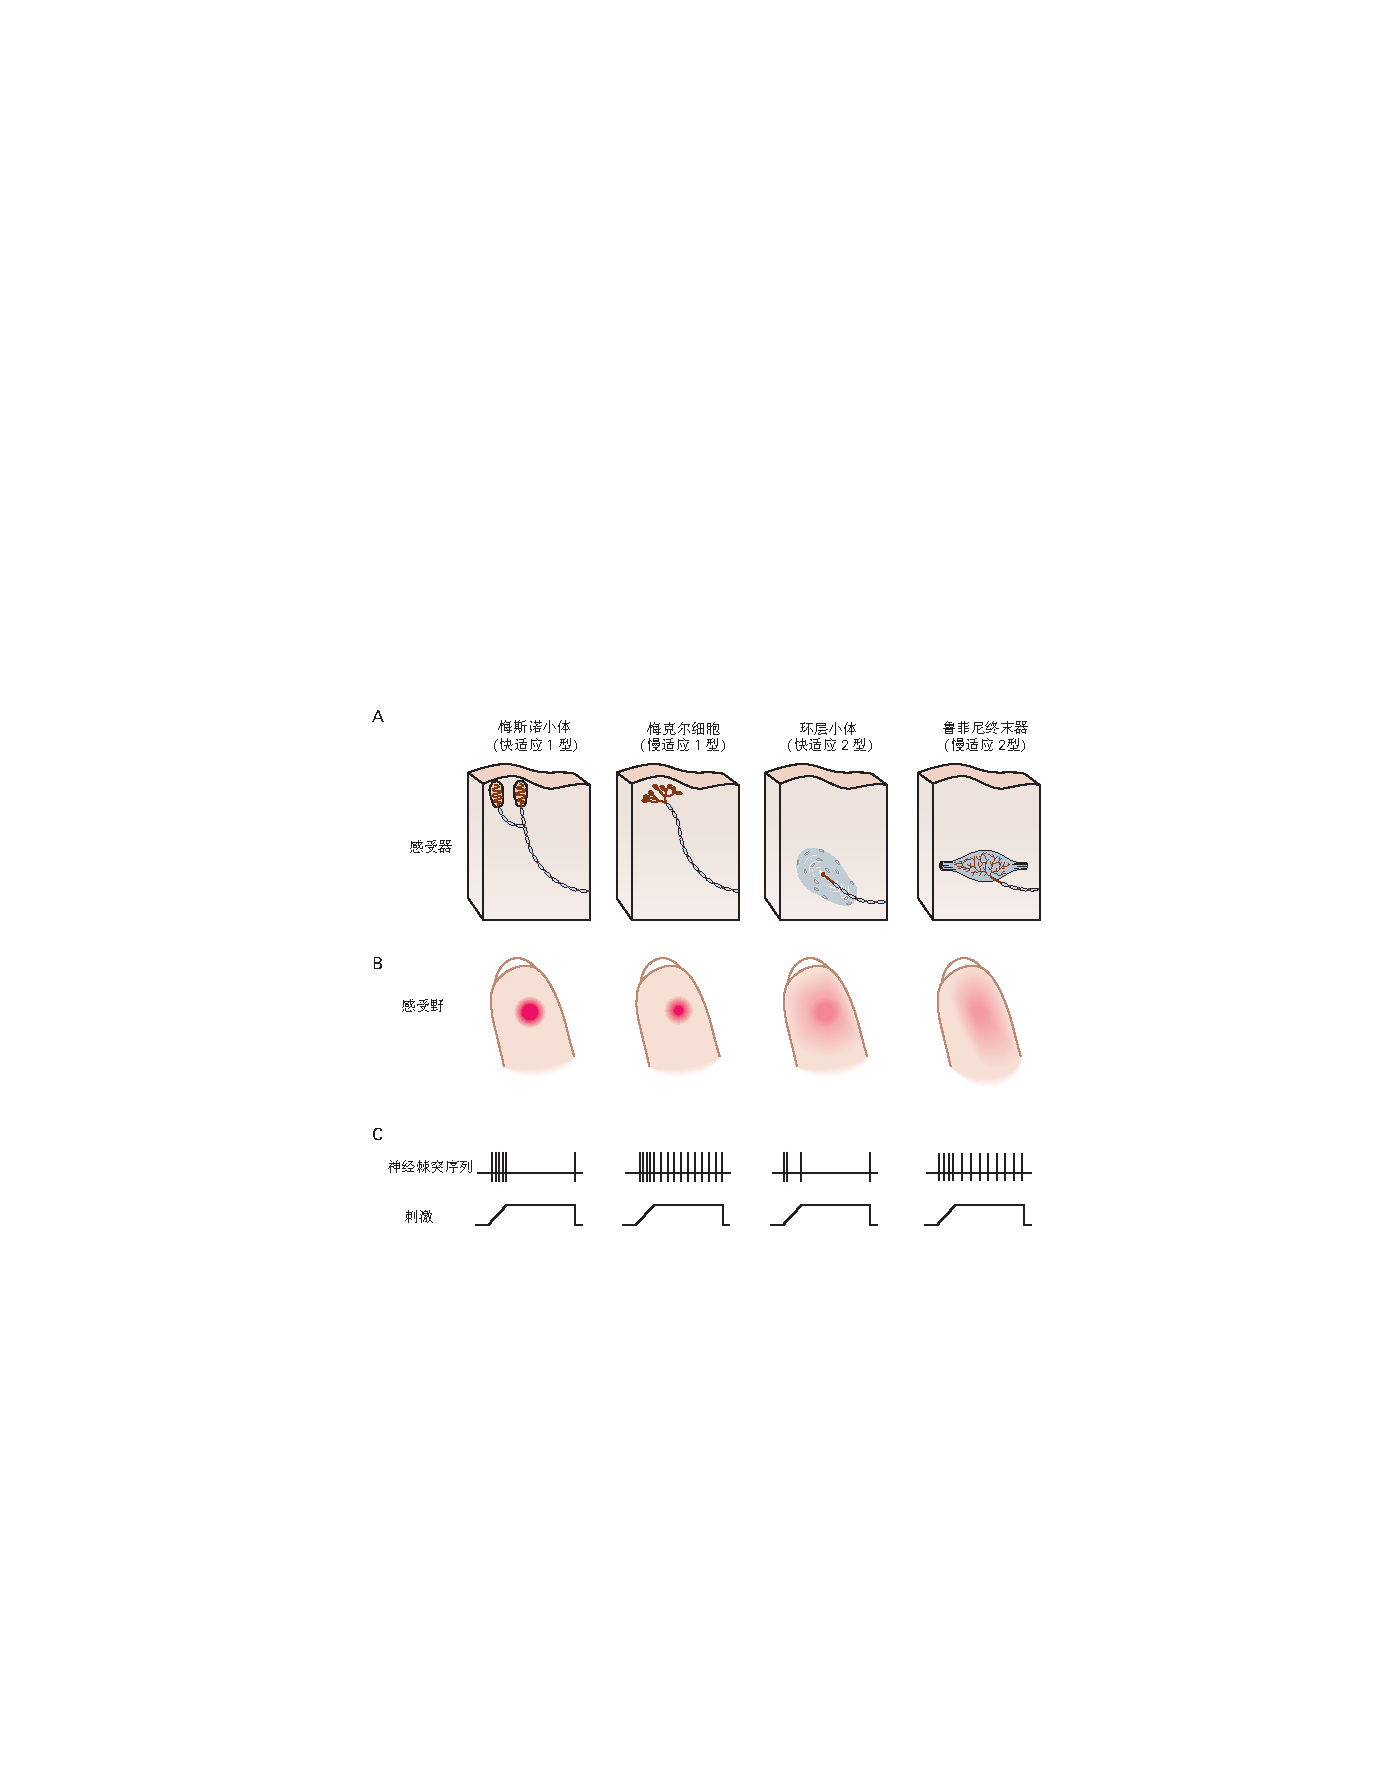
\includegraphics[width=0.95\linewidth]{chap19/fig_19_1}
	\caption{四种类型的机械感受器负责人手的触觉。
		支配手部的有髓感觉神经的末端被专门的结构包围,这些结构可以检测皮肤上的接触。
		这些受体在形态、神经支配模式、皮肤位置、感受野大小和对触摸的生理反应方面各不相同\cite{johansson1983tactile}。
		\textbf{A.} 手部无毛(无毛)皮肤的表层和深层各包含不同类型的机械感受器。
		表层包含小受体细胞:迈斯纳小体(\textit{快适应1型})和默克尔细胞(\textit{慢适应1型})。
		支配这些受体的感觉神经纤维具有支配一种类型的多个受体的分支末端。
		皮肤和皮下组织的深层包含大受体:\textit{环层小体}(\textit{快适应2型})和\textit{鲁菲尼终末器}(\textit{慢适应2型})。
		这些感受器中的每一个都由一根神经纤维支配,而每根纤维仅支配一个感受器。
		\textbf{B.} 机械感受器的感受野反映了其末端在皮肤中的位置和分布。
		皮肤表层的触觉感受器比深层的感受器具有更小的感受野。
		\textbf{C.} 支配每种机械感受器的神经纤维在被激活时的反应不同。
		尖峰序列示意图显示了当通过缓慢增加和恒定的对皮肤的压力激活其受体时,每种类型的神经的反应。
		\textit{快适应}纤维在压力刺激开始和结束时对运动做出反应,并迅速适应持续的刺激,而缓慢适应的纤维对稳定的压力和运动都有反应,并缓慢适应。}
	\label{fig:19_1}
\end{figure}


触觉感受器由缓慢适应或\textit{快适应}的轴突支配。
\textit{慢适应}纤维通过持续放电响应稳定的皮肤压痕,而\textit{快适应}纤维在压痕变得静止时停止放电(图~\ref{fig:19_1}~和表~\ref{tab:19_1})。
手部持续的机械感觉必须相应地从\textit{慢适应}纤维中产生;
皮肤上或穿过皮肤的运动感觉主要由\textit{快适应}纤维发出信号。


\begin{table}[htbp]
	\caption{无毛皮肤中的皮肤机械感受器} \label{tab:19_1} \centering
	\begin{tabular}{lllll}
		\toprule
		 & 类型 1 &  & 类型 2 & \\
		 \toprule
		 & 慢适应类型 1 & 快适应类型 1  & 慢适应类型 2 & 快适应类型 2 \\
		\midrule
		受体 & \makecell[l]{梅克尔细胞/\\轴突复合体\\(多末端)} & \makecell[l]{梅斯诺小体\\(多末端)} & \makecell[l]{鲁菲尼终末器\\(单末端)} & \makecell[l]{环层小体\\(单末端)} \\
		位置 & \makecell[l]{围绕汗腺的\\中间脊底部} & \makecell[l]{真皮乳头(\\邻近限制脊)} & \makecell[l]{皮肤褶皱、关节\\处皮肤、指甲床} & \makecell[l]{真皮(\\深层组织)} \\
		\makecell[l]{轴突直径\\(微米)} & 7-11 & 6-12 & 6–12 & 6–12 \\
		\makecell[l]{传导速度\\(毫秒)} & 40–65 & 35–70 & 35–70 & 35–70 \\
		最佳刺激 & 边、点 & 横向运动 & 皮肤拉伸 & 震动 \\
		\makecell[l]{对持续压\\痕的反应} & \makecell[l]{持续且适应\\缓慢(不规则\\激活模式)} & \makecell[l]{刺激开始\\时的阶段性} & \makecell{持续且适应\\缓慢(正常\\激活速率)} & \makecell[l]{刺激开始\\时的阶段性} \\
		\bottomrule
	\end{tabular}
\end{table}


手上的触觉感受器根据大小和在皮肤中的位置进一步细分为两种类型。
1 型触觉纤维终止于真皮和表皮之间边缘皮肤表层的小受体器官簇(迈斯纳小体或默克尔细胞)(图~\ref{fig:19_2},方框~\ref{box:19_1})。
\textit{快适应}1 纤维是手部数量最多的触觉传入神经,在人和猴子的指尖处达到约 150 个每平方厘米的密度;
\textit{慢适应1型}纤维也广泛分布在手中,指尖的密度为每平方厘米 70 根。


\begin{proposition}[指纹结构提高了手部的触摸灵敏度] \label{box:19_1}
	
	\quad \quad 无毛皮肤的组织结构(手掌和指尖光滑无毛的皮肤)在手对触摸的敏感性中起着至关重要的作用。
	指纹是由表皮中平行脊的规则阵列形成的,即乳头脊(图~\ref{fig:19_3})。
	从每个脊的中心出现的汗腺下方规则间隔的\textit{梅克尔细胞}提供了一个空间网格,使我们能够准确地将刺激定位在指尖上。
	
	\quad \quad 每个脊都有表皮褶皱(限制脊),在手指、手掌和脚上可以看到细线。
	限制性隆起增加了皮肤的硬度和硬度,保护皮肤在接触物体或赤脚行走时免受损伤。
	迈斯纳小体通常位于真皮乳头中,靠近限制嵴;
	每个毛乳头包含几个迈斯纳小体,并由两到五个\textit{快适应1型}轴突支配(图~\ref{fig:19_4})。
	
	\quad \quad \textit{梅克尔细胞}由\textit{慢适应 1 型}纤维支配,密集地聚集在每个乳头嵴的中心,位于表皮汗腺管周围的中间嵴的底部(图~\ref{fig:19_4}A),使它们处于一个很好的位置,可以检测表皮因压力或侧向拉伸而变形。
	它们的触觉感受功能与毛皮肤触摸圆顶中的\textit{梅克尔细胞}相似(第~\ref{chap:chap18}~章)。
	
	\quad \quad 指纹使无毛的皮肤具有波纹状、粗糙的结构,增加了摩擦力,使我们能够在不打滑的情况下抓住物体。
	当这些脊与物体的纹理表面接触时,摩擦力进一步增加。
	光滑的表面很容易在手指下方滑动,因此需要更大的握力来保持手部的稳定性;瓶子上的螺帽通常是脊状的,以便于转动。
	当我们触摸物体时,限制脊和物体之间的摩擦力也会放大我们对表面特征的感觉,产生振动,使我们能够检测到微小的不规则性,如木纹和织物线。
	
	\quad \quad 乳头嵴的规则间距(以及特定受体在该网格内的精确定位)使我们能够通过手的来回运动反复扫描表面,同时保持相邻表面特征的恒定空间对齐。
	它们还提供了一个解剖网格,用于参考触觉刺激的精确位置。
	
\end{proposition}


\begin{figure}[htbp]
	\centering
	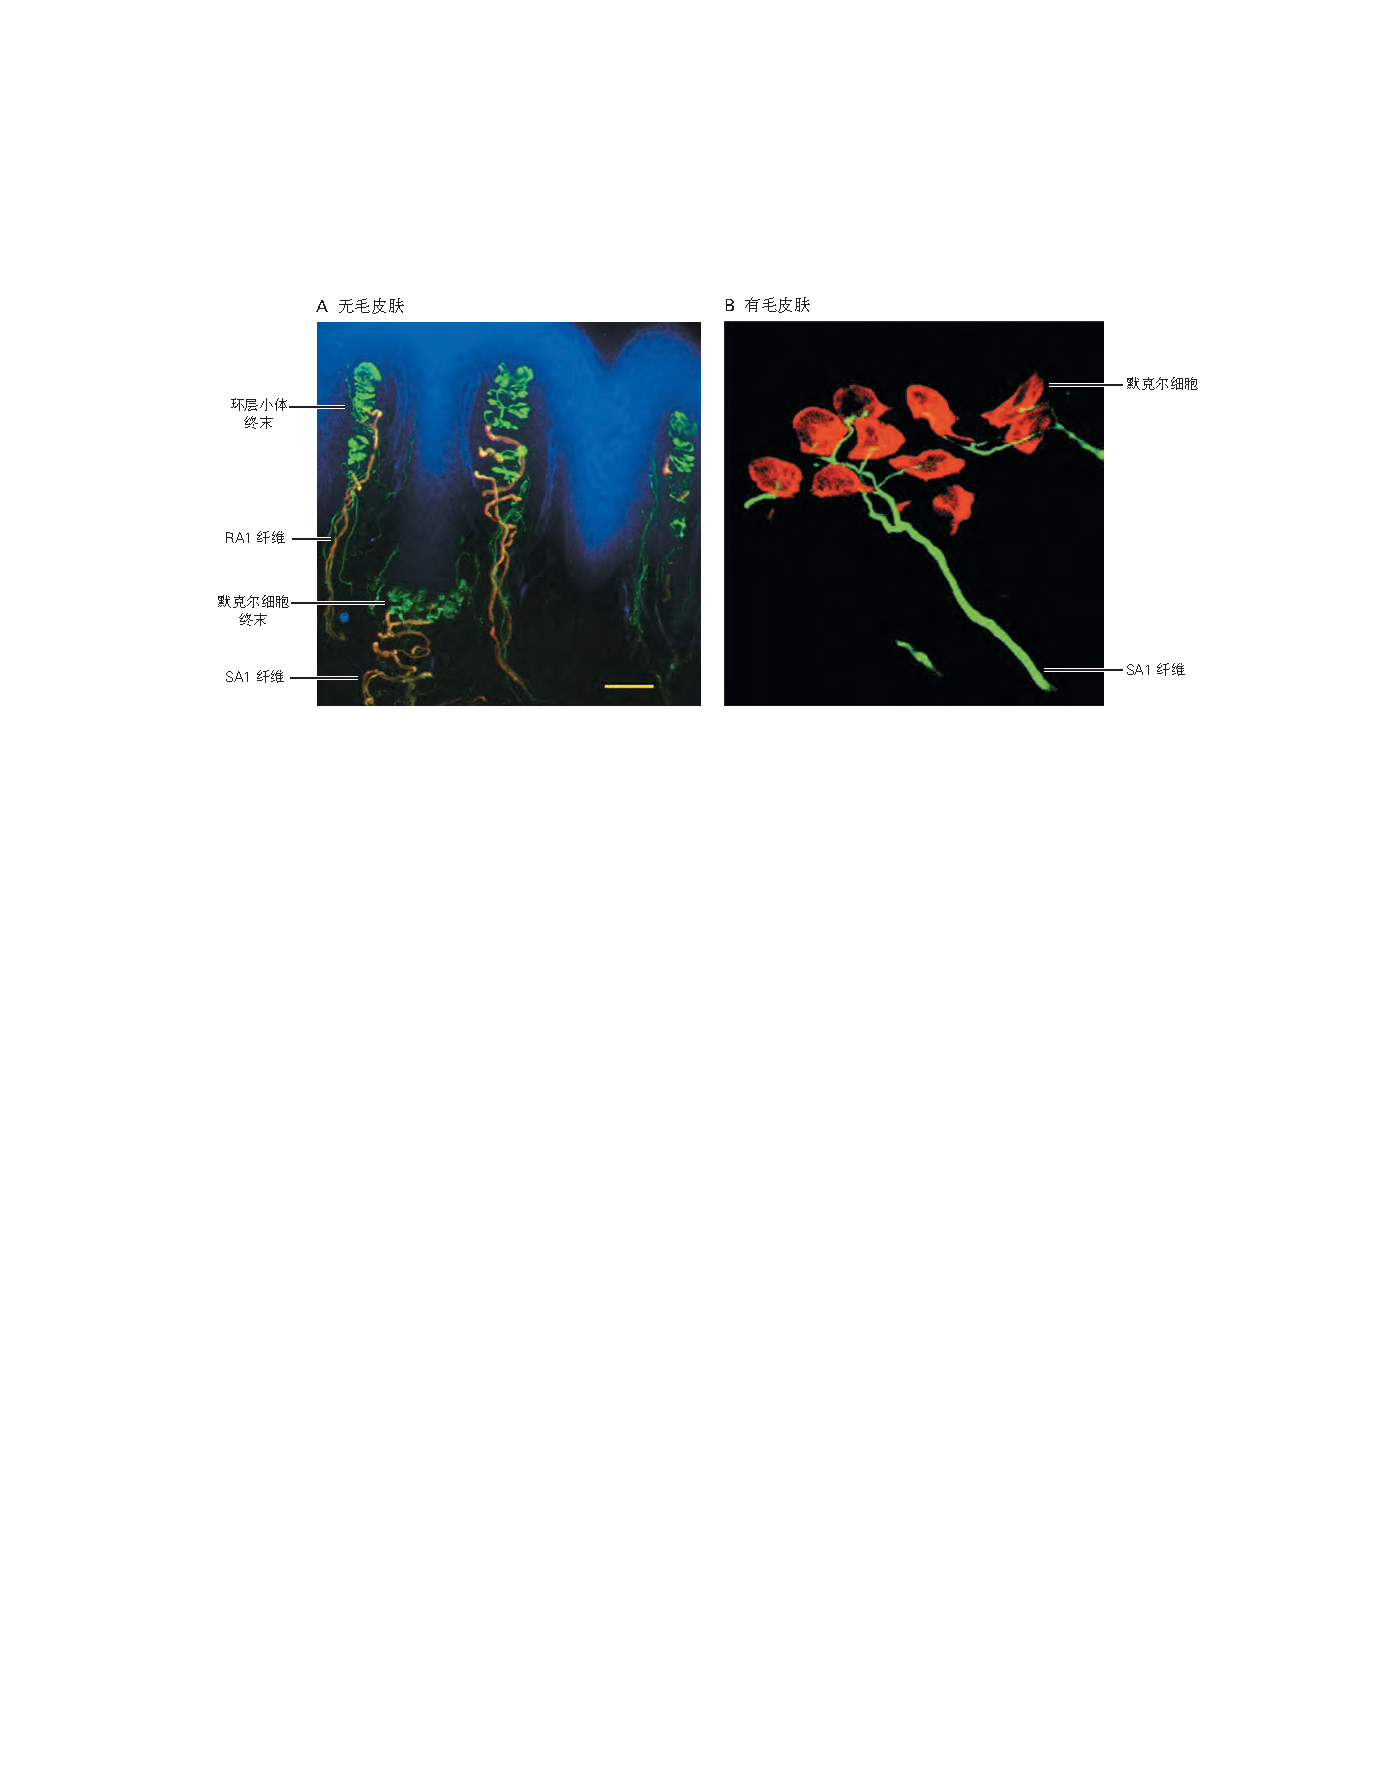
\includegraphics[width=1.0\linewidth]{chap19/fig_19_4}
	\caption{无毛和有毛皮肤中迈斯纳小体和默克尔细胞的神经支配模式。
		\textbf{A.} 人类指尖皮肤乳头嵴的共焦横截面显示了机械感受器的神经支配模式。
		迈斯纳小体位于真皮乳头中,位于与限制嵴交界的表皮(蓝色)正下方,由两种或多种\textit{快适应1型}纤维支配。
		当纤维进入受体膜时,它们失去了髓鞘(橙色),暴露出广泛的末端球茎(绿色),在那里发生感觉转导。
		单个\textit{慢适应 1 型}纤维支配聚集在中间嵴底部的\textit{梅克尔细胞}群,提供施加到该嵴的局部压力信号。比例尺=50微米。}
		\textbf{B.} 更高倍率的显微照片描绘了角蛋白-8抗体标记的\textit{梅克尔细胞}(红色),其由标记有神经丝重多肽(NFH+)的\textit{慢适应 1 型}纤维(绿色)支配。
		每个神经纤维平行于皮肤表面延伸多个分支,使其能够整合来自皮肤小区域中多个受体细胞的触觉信息。
		每个\textit{梅克尔细胞}的直径约为10微米。
	\label{fig:19_4}
\end{figure}


2 型纤维稀疏地支配皮肤并终止于位于真皮或皮下组织中的单个大受体(\textit{环层小体}和\textit{鲁菲尼终末器})。 
这些受体比 1 型纤维的受体器官更大但数量更少。
2 型受体的大尺寸使它们能够在距感觉神经末梢一定距离处感知皮肤的机械位移。
人手指中\textit{快适应}2纤维的密度仅为每平方厘米21根;
\textit{慢适应2型}纤维含量最少,每平方厘米仅提供 9 根纤维。


\begin{figure}[htbp]
	\centering
	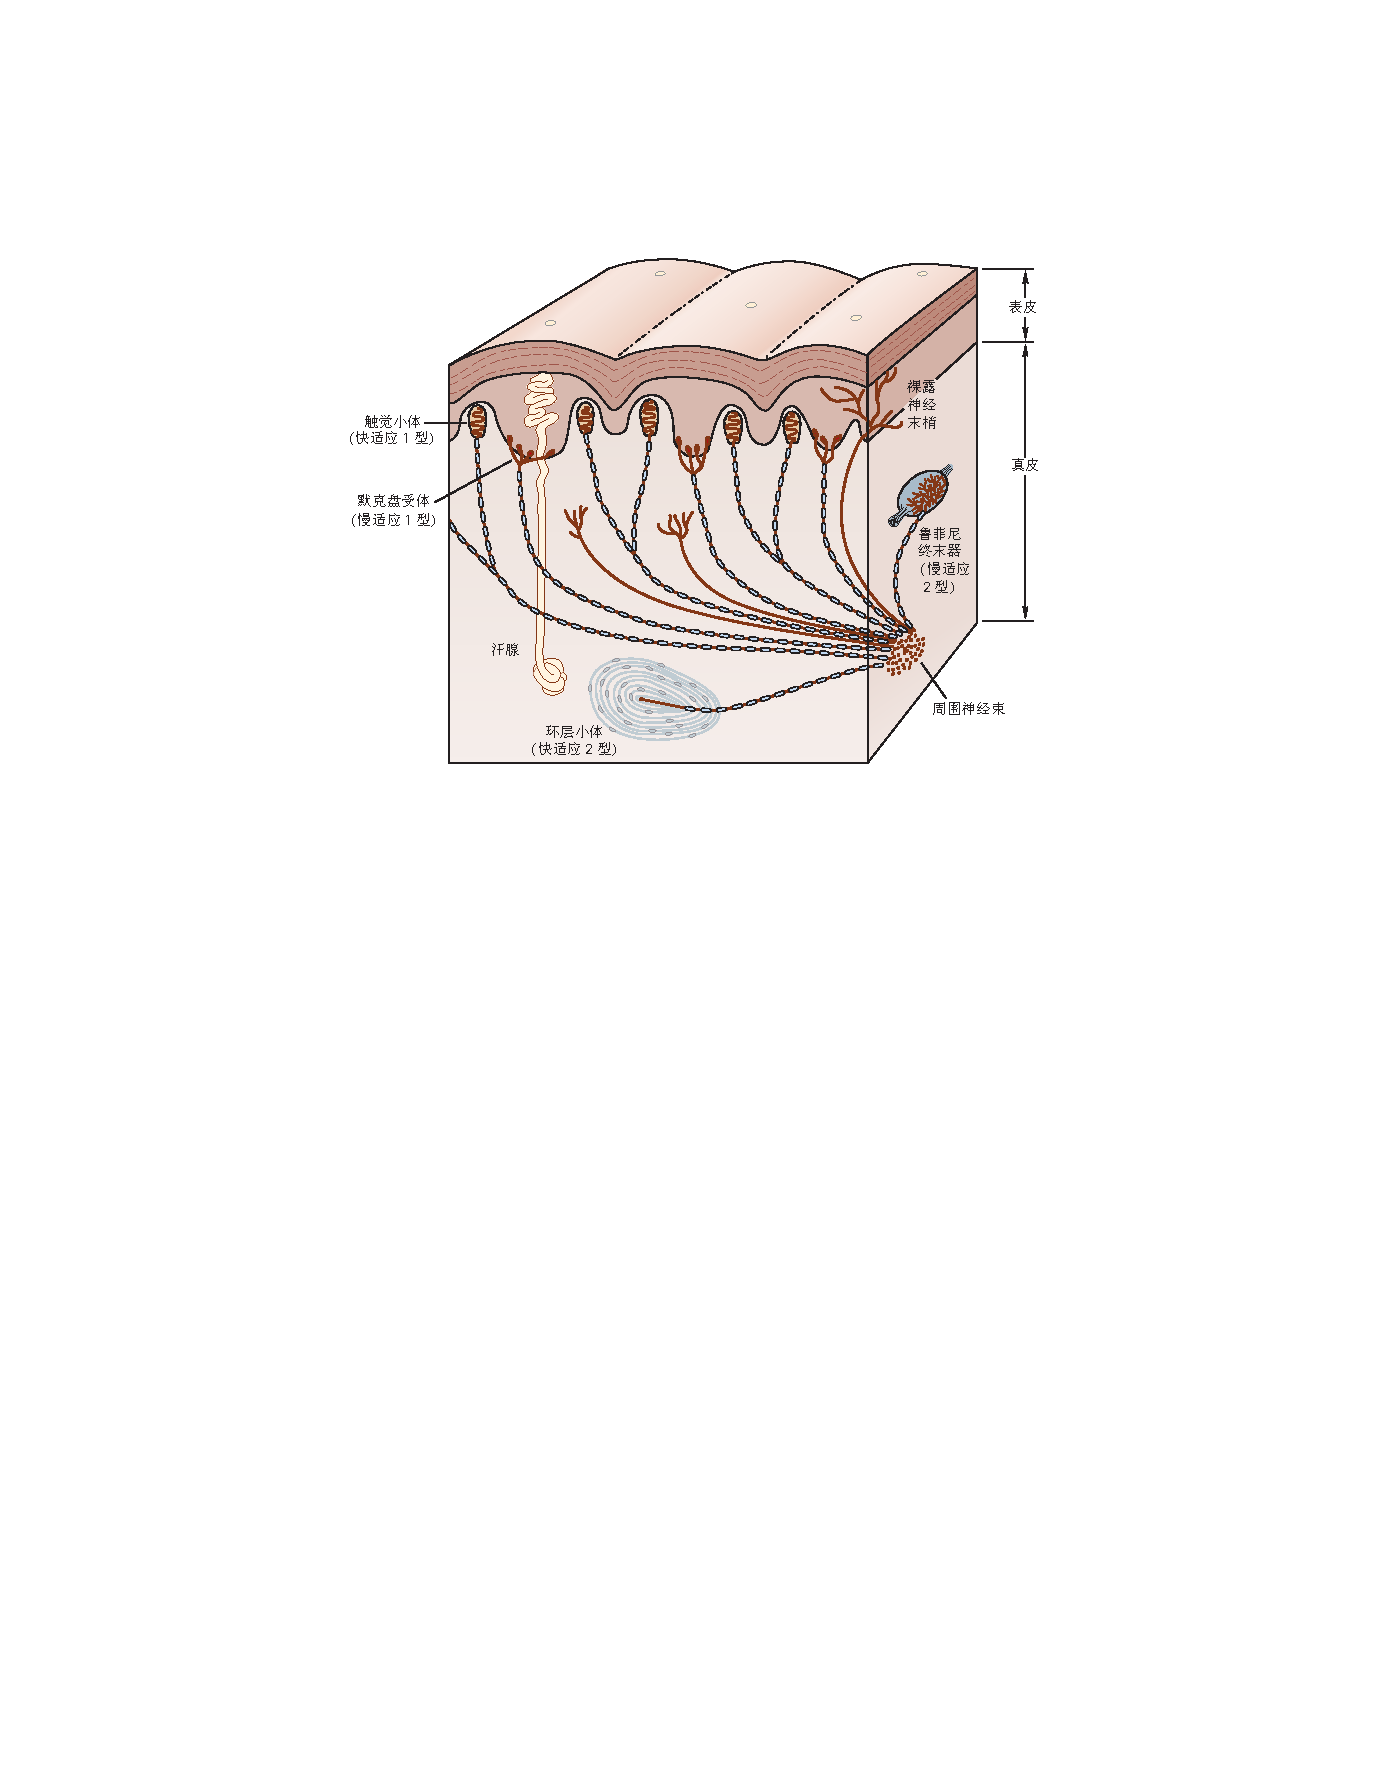
\includegraphics[width=0.85\linewidth]{chap19/fig_19_2}
	\caption{人类无毛皮肤的触觉神经支配。
		无毛皮肤的横截面显示了人手触摸的主要受体。
		所有这些受体均受大直径A$\beta$髓鞘纤维的支配。
		\textit{梅斯诺小体}和\textit{梅克尔细胞}位于表皮底部的皮肤表层,距离皮肤表面0.5至1.0毫米。
		梅斯纳小体位于毛乳头中,与每个乳头脊的边缘接壤。默克尔细胞沿着乳头状脊的中心在汗腺导管周围的中间脊下方形成致密带。
		支配这些受体的\textit{快适应1型}和\textit{慢适应1型}纤维在其末端分支,因此每根纤维都支配附近的几个受体器官。
		\textit{环层小体}和\textit{鲁菲尼终末器}位于真皮内(2-3毫米厚)和更深的组织中。
		支配这些受体的\textit{快适应2型}和\textit{慢适应2型}纤维各自仅支配一个受体器官。}
	\label{fig:19_2}
\end{figure}


\begin{figure}[htbp]
	\centering
	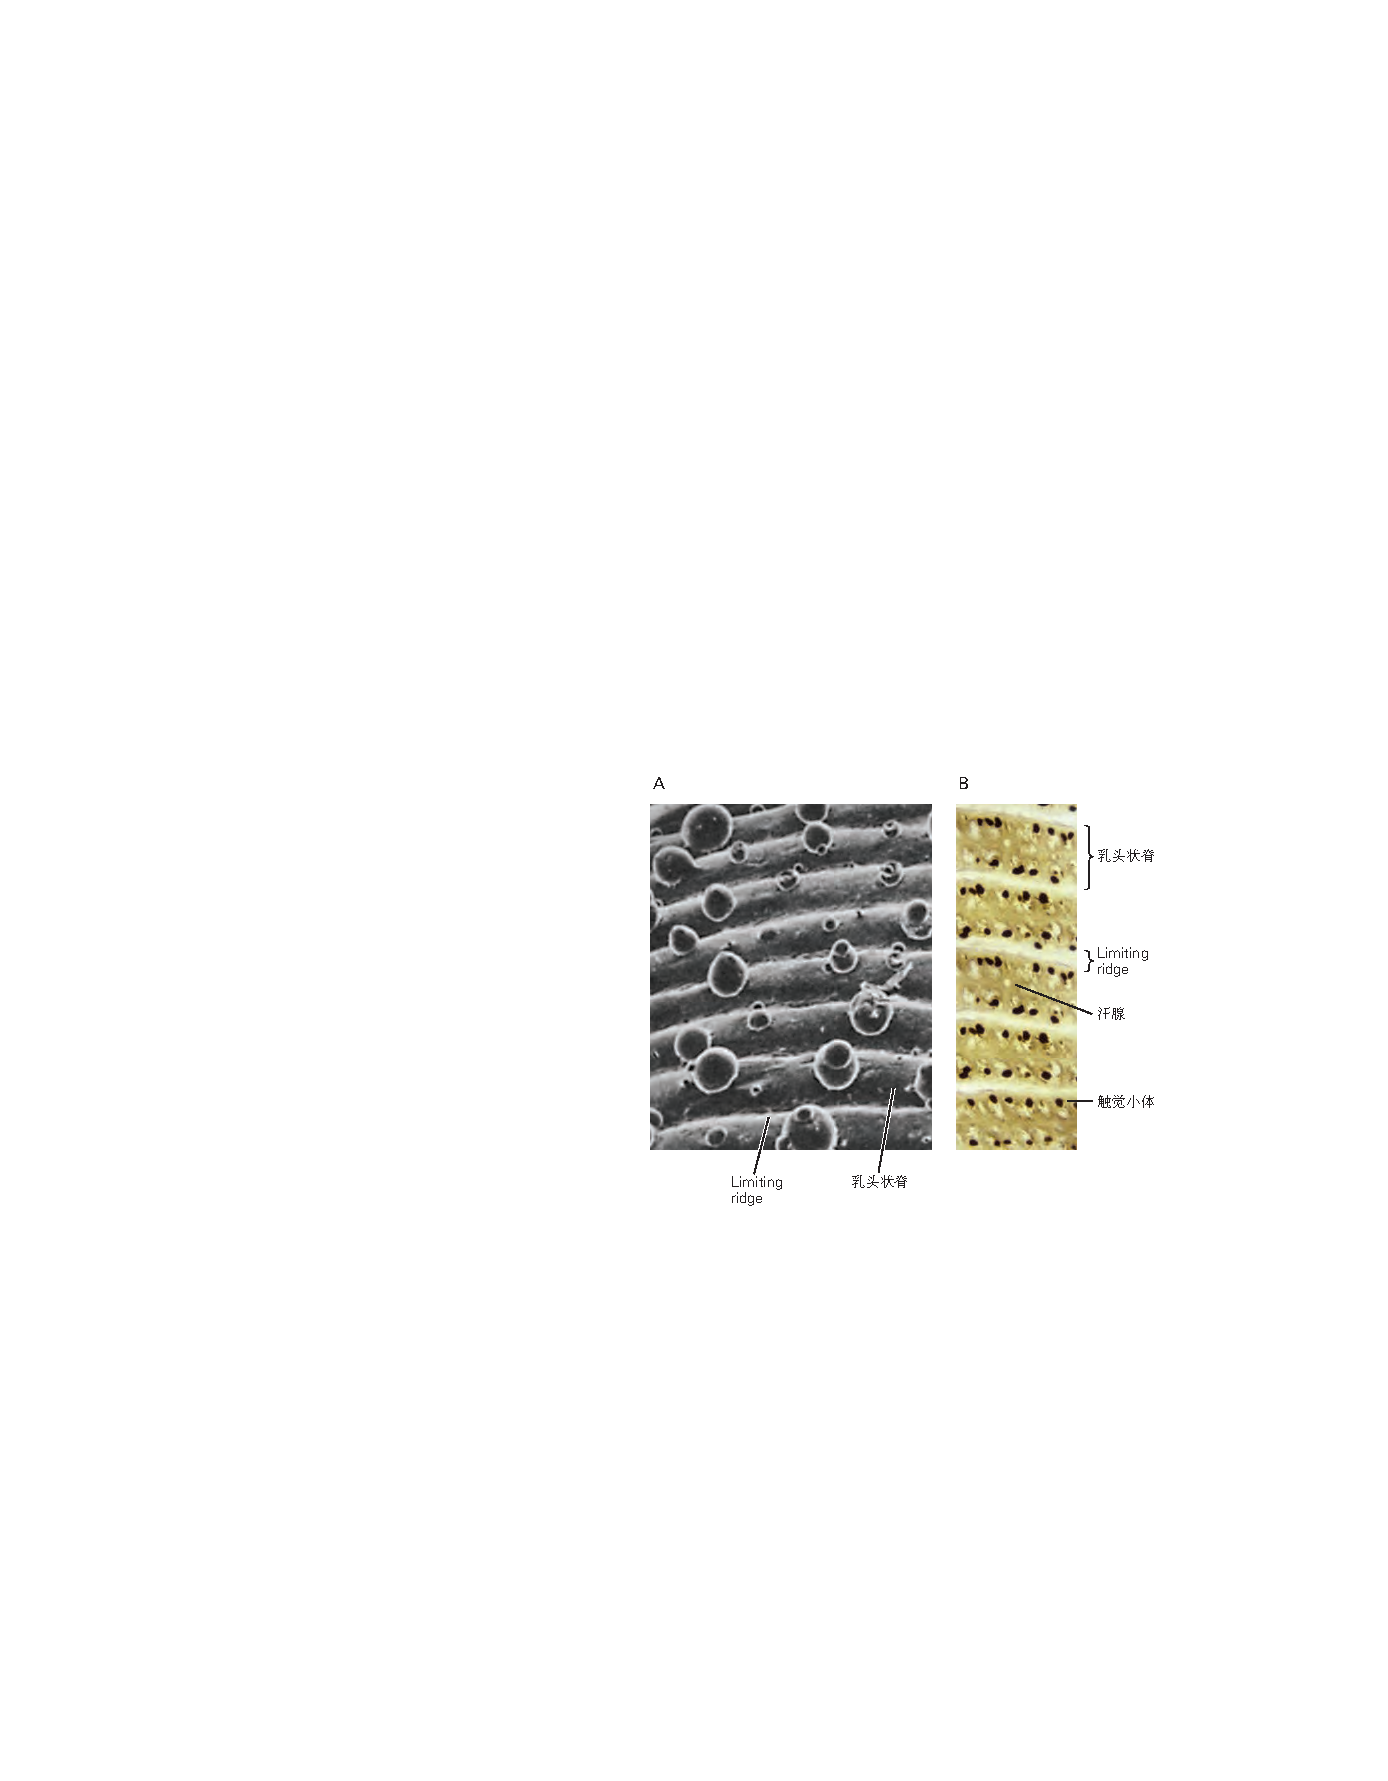
\includegraphics[width=0.7\linewidth]{chap19/fig_19_3}
	\caption{人类指尖的皮肤。
		\textbf{A.} 人类食指指纹的扫描电子显微照片。
		手部的无毛皮肤由\textit{乳头状脊}和间隔有规律的沟(\textit{限制脊})排列而成。
		汗珠从\textit{乳头状脊}中心的导管中渗出,沿着每个隆起的中心形成规则间隔的网格状图案。
		\textit{梅克尔细胞}位于表皮底部汗管下方的密集簇中,沿着\textit{乳头状脊}的中心(见图~\ref{fig:19_2})。
		 \textbf{B.} 平行于皮肤表面切割的无毛皮肤的组织切片。
		 此处对胆碱酯酶进行免疫染色的迈斯纳小体沿着与限制脊相邻的每个乳头状脊的两侧形成规则间隔的链。
		 因此,\textit{梅斯诺小体}和\textit{梅克尔细胞}形成交替的\textit{快适应 1 型}和\textit{慢适应1型}触摸感受器带,跨越每个指纹脊\cite{bolanowski2003organization}。}
	\label{fig:19_3}
\end{figure}



\subsection{细胞的感受野决定了它的触觉敏感区}

单个机械感受器纤维从称为感受野的有限皮肤区域传递信息(第~\ref{chap:chap18}~章)。
\textit{亚克$\cdot$威尔波}和\textit{罗兰$\cdot$约翰逊}首先使用显微神经描记术研究了人手的触觉感受野。
他们通过皮肤将微电极插入人类前肢的正中神经或尺神经,并记录单个传入纤维的反应。
他们发现,与其他灵长类动物一样,人类的触觉感受器在生理反应和感受野结构方面都存在重要差异。


1 型纤维具有小的、高度局部化的感受野,具有多个高灵敏度点,反映了它们在皮肤中的轴突末端的分支模式(图~\ref{fig:19_5})。
一个\textit{快适应}1轴突通常支配 10 到 20 个迈斯纳小体,整合来自几个相邻指纹脊的信息。
一根\textit{慢适应1型}纤维支配年轻人中大约 20 个\textit{梅克尔细胞}(图~\ref{fig:19_4}B);
随着年龄的增长,默克尔细胞的数量会显著下降。


\begin{figure}[htbp]
	\centering
	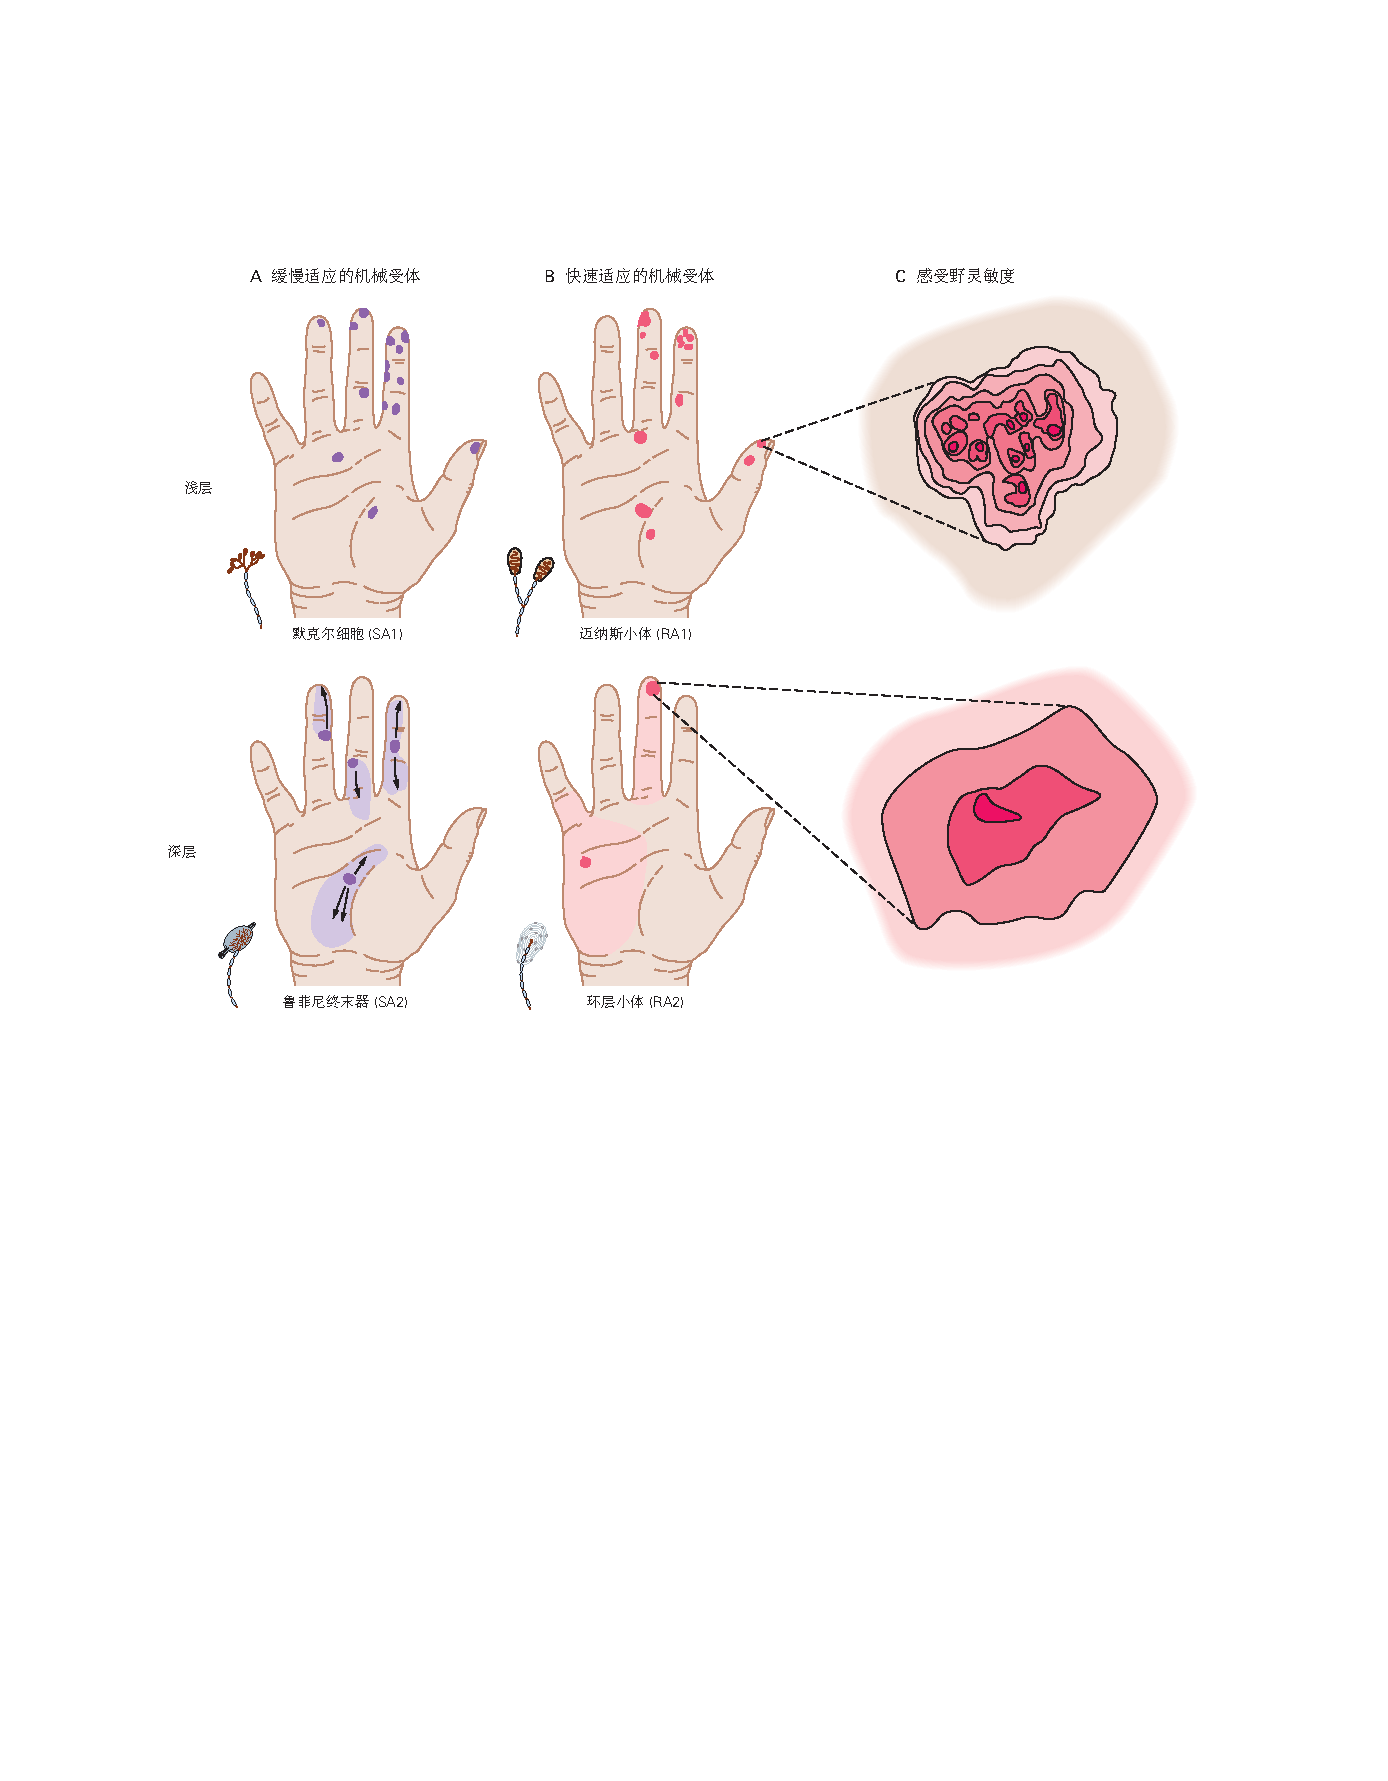
\includegraphics[width=1.0\linewidth]{chap19/fig_19_5}
	\caption{人手的感受野在指尖处最小。
		手上的每个彩色区域表示单个感觉神经纤维的感受野\cite{johansson1983tactile}。
		在皮肤表层,1 型受体的感受野包括斑点状皮肤斑块。
		在深层,2 型感受野延伸到广泛的皮肤区域(浅色阴影),但直接在感受器上方的皮肤(黑点)的反应最强。 
		箭头指示激活\textit{慢适应2型}纤维的皮肤拉伸方向。
		\textbf{C.} 整个感受野的压力敏感度显示为等高线图。
		最敏感的区域以深红色表示,最不敏感的区域以淡粉色表示。
		\textit{快适应} 1 型纤维(上图)的感受野有许多高灵敏度点,标记了由纤维支配的迈斯纳小体群的位置。
		\textit{快适应} 2 型纤维(下图)的感受野在\textit{环层小体}上有一个最大灵敏度的单点。
		\textit{慢适应 1 型}纤维的感受野等高线图与\textit{快适应}1 纤维相似。
		同样,\textit{慢适应2型}纤维的感受野图与 \textit{快适应}2 纤维相似。}
	\label{fig:19_5}
\end{figure}


相比之下,支配皮肤深层的 2 型纤维仅与单个\textit{环层小体}或\textit{鲁菲尼终末器}相连。
由于这些受体很大,它们从更广泛的皮肤区域收集信息。 
他们的感受野通常包含一个单一的“热点”,那里对触摸的敏感度最高;
该点位于接收器的正上方(图~\ref{fig:19_5})。


指尖的感受野在身体上是最小的,\textit{慢适应1型}纤维平均为 11 平方毫米,\textit{快适应} 1型 纤维平均为 25 平方毫米。
小场补充了指尖中高密度的感受器。
近端指骨和手掌的感受野逐渐变大,这与这些区域的机械感受器密度较低一致。
重要的是,1 型纤维的感受野明显小于大多数接触手的物体,因此仅表示物体有限部分的空间特性。
与视觉系统一样,物体的空间特征分布在受刺激的受体群中,这些受体的反应在大脑中整合形成统一的感知。


每个\textit{快适应} 2 型轴突在没有分支的情况下终止于单个\textit{环层小体},并且每个 \textit{环层小体}只接受一个\textit{快适应} 2 型轴突。
\textit{环层小体}是大的洋葱状结构,其中连续的结缔组织层被充满液体的空间隔开(见图~\ref{fig:19_8}A1)。
这些层围绕着无髓鞘的\textit{快适应 2 型} 末端及其有髓鞘的轴突,直至一个或多个朗飞节。
胶囊会放大高频振动,这一作用对于工具的使用非常重要。
据估计,人手中的帕西尼氏小体数量从年轻人的 2,400 个到老年人的 300 个不等。


\textit{慢适应2型}纤维支配\textit{鲁菲尼终末器},集中在手指和腕关节、指甲周围的皮肤以及手掌的皮肤褶皱处。
\textit{鲁菲尼终末器}是细长的纺锤形结构,包围着从皮下组织延伸到关节、手掌或指甲边缘处皮肤褶皱处的胶原纤维。
\textit{慢适应2型}神经末梢缠绕在囊中的胶原纤维之间,就像在高尔基肌腱器官中一样(方框~\ref{box:32_4}),并被沿其长轴拉伸皮肤的刺激所兴奋。



\subsection{两点辨别测试测量触觉敏锐度}

人类分辨纹理表面空间细节的能力取决于接触身体的哪个区域。
当一对探针在手上相距几毫米时,每个探针都被视为一个不同的点,因为它在皮肤上产生一个单独的酒窝并刺激不重叠的受体群。
当探头靠得更近时,两种感觉会变得模糊,因为两个探头都包含在相同的感受野中。
触觉刺激之间的空间相互作用构成了两点辨别和纹理识别的神经学测试的基础。


触觉敏锐度的阈值(定义机会和完美辨别之间性能的分离)在年轻人的指尖上约为 1 毫米,但在老年人中下降到约 2 毫米。
指尖和嘴唇的触觉敏锐度最高,感受野最小。
身体近端部位的触觉敏锐度随着\textit{慢适应1型}和\textit{快适应 1 型}纤维感受野的大小而降低(图~\ref{fig:19_6}A)。


\begin{figure}[htbp]
	\centering
	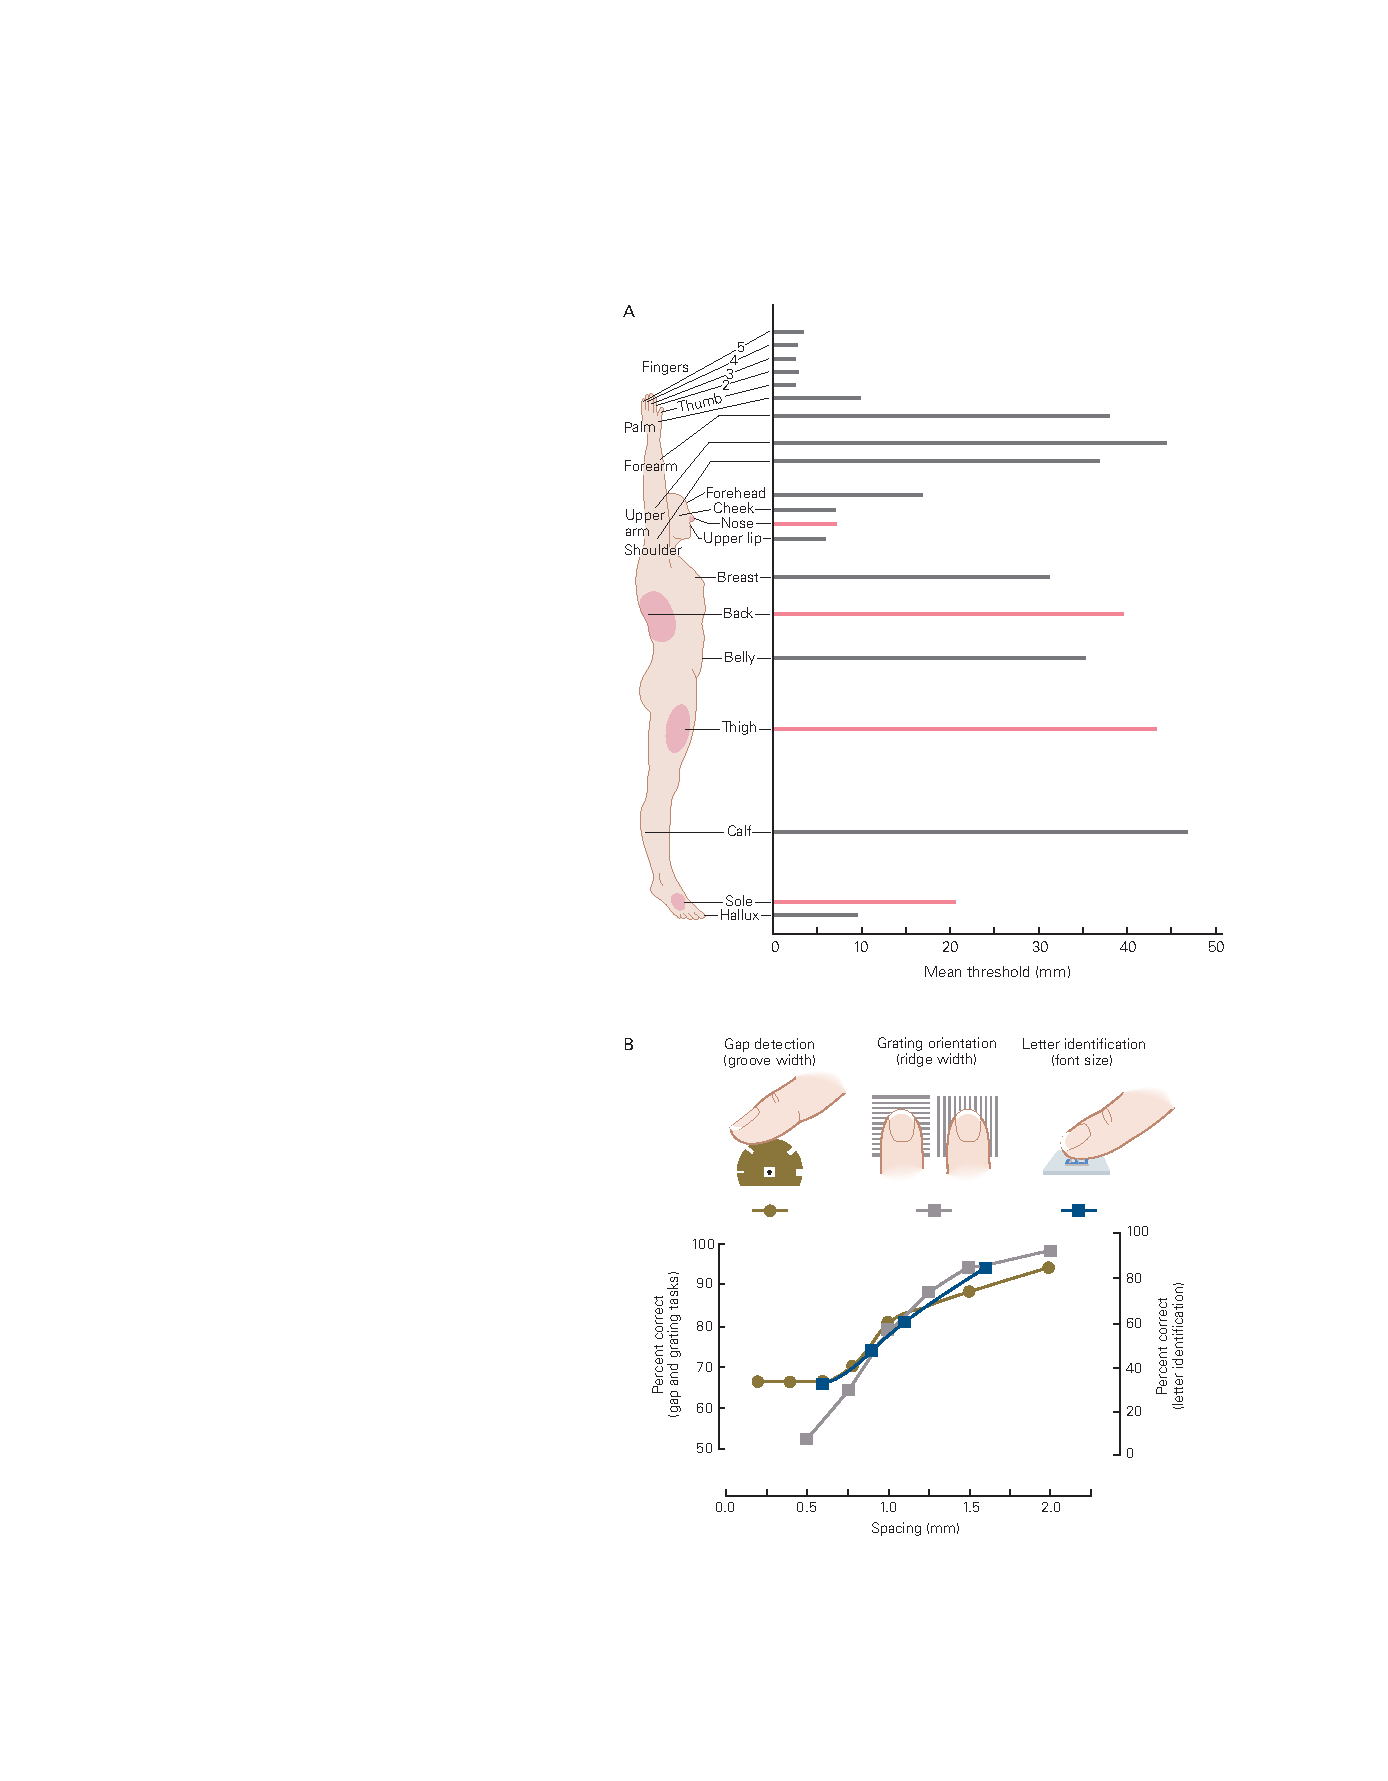
\includegraphics[width=1.0\linewidth]{chap19/fig_19_6}
	\caption{人手的触觉敏锐度在指尖最高。
		\textbf{A.} \textit{两点阈值}测量两个刺激被分辨为不同的最小距离。
		该距离因身体不同部位而异;
		它在手指上约为 2 毫米,但在手掌上可达 10 毫米,在手臂、大腿和背部可达 40 毫米。
		不同身体部位的平均两点感知阈值,由条形图中的粉红色线条表示,与身体上相应粉红色区域的平均感受野直径相匹配。
		指尖、嘴唇和舌头具有最大的辨别能力,它们具有最小的感受野\cite{weinstein1968intensive}。
		\textbf{B.} 空间敏锐度是在心理物理学实验中通过让被蒙住眼睛的受试者触摸各种纹理表面来测量的。
		如图所示,受试者被要求确定轮子的表面是光滑的还是有缝隙,光栅的脊线是横跨手指还是平行于手指的长轴,或者哪些字母出现在凸起的字体上活版印刷。
		触觉敏锐度阈值定义为产生 75\% 正确性能的凹槽宽度、脊宽度或字体大小(在偶然和完美准确度之间可检测到的中间值)。
		在每个测试中,人类指尖的阈值间距为 1.0 毫米\cite{johnson1981tactile}。}
	\label{fig:19_6}
\end{figure}


当我们抓住或触摸一个物体时,我们可以辨别其表面的特征,相隔小至 0.5 毫米。
人类能够区分脊间距非常窄的光栅的水平和垂直方向(图~\ref{fig:19_6}B)。
长边,如光栅的脊,在同时刺激感受野中的多个感觉末梢时会引起\textit{快适应1型}和\textit{慢适应1型}1传入神经的更强反应,强调多传感器感受野对触觉信息处理的重要性。
\textit{罗兰$\cdot$约翰逊}和\textit{安德鲁$\cdot$普鲁斯钦斯基}最近发现,\textit{快适应1型}和\textit{慢适应1型}纤维对接触多个感觉末梢的边缘反应更强烈,使这些传入神经能够区分垂直、水平或倾斜方向。


女性的触觉敏锐度略高于男性,并且在手指之间存在差异,但在手之间没有差异;
性别差异主要与女性乳头嵴直径较小以及由此导致的每平方厘米皮肤\textit{慢适应1型}1纤维密度较高有关。
食指的远端垫具有最敏锐的灵敏度;
空间敏锐度从食指到小指逐渐下降,并在靠近远端指垫的位置迅速下降。
小指远端的触觉空间分辨率较差 50\%,手掌较粗糙 6 到 8 倍。


盲人使用\textit{慢适应1型}和\textit{快适应1型}纤维的精细空间灵敏度来阅读盲文。
盲文字母表将字母表示为易于通过触摸区分的简单圆点图案。
盲人通过在圆点图案上移动手指来阅读盲文。
这种手部运动增强了点产生的感觉。
由于盲文点之间的间距约为 3 毫米,该距离大于\textit{慢适应1型}纤维的感受野直径,因此每个点刺激一组不同的\textit{慢适应1型}纤维。
当一个点进入它的感受野时,\textit{慢适应1型}纤维会发出一阵动作电位,而一旦该点离开感受野,它就会停止活动(图~\ref{fig:19_7})。
同步发射的\textit{慢适应1型}纤维的特定组合发出盲文点的空间排列信号。
\textit{快适应1型}纤维还区分点图案,增强\textit{慢适应1型}纤维提供的信号。


\begin{figure}[htbp]
	\centering
	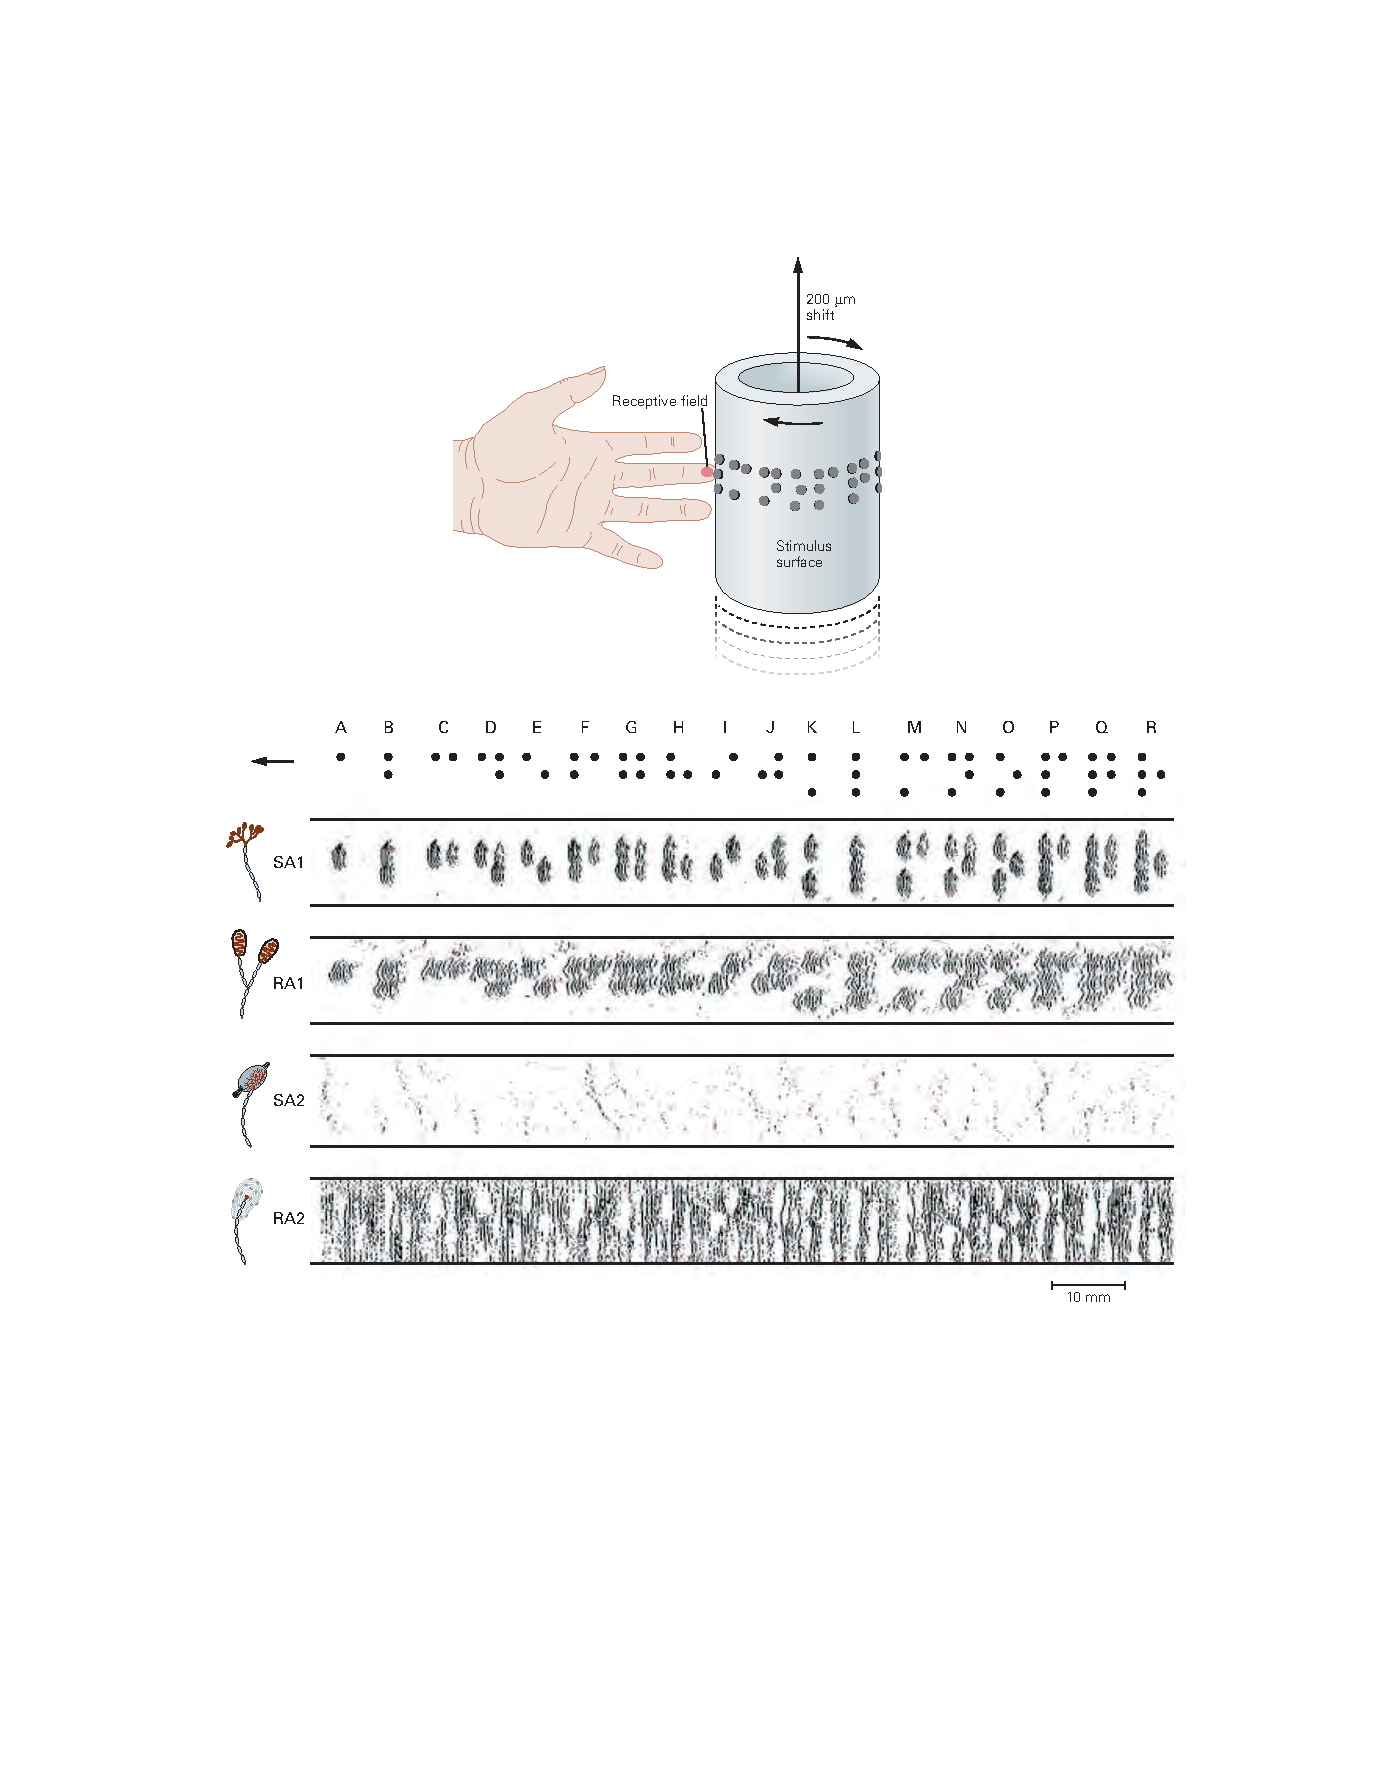
\includegraphics[width=1.0\linewidth]{chap19/fig_19_7}
	\caption{触摸感受器对手指扫描的盲文点的反应。
		字母 A 到 R 的盲文符号安装在一个鼓上,该鼓在人类受试者的指尖上反复旋转。
		每次旋转后,鼓向上移动,以便在手指上扫描另一部分符号。
		放置在该受试者正中神经中的微电极记录了支配指尖的机械感受纤维的反应。
		当盲文符号在感受野上移动时,神经纤维释放的动作电位在这些记录中用小点表示; 每个水平行的点代表纤维对鼓的单次旋转的响应。
		\textit{慢适应1型}受体记录了盲文符号最清晰的图像,用一系列动作电位代表每个盲文点,当盲文符号之间的空间不提供刺激时,它们就会变得安静。
		\textit{快适应1型}受体提供盲文符号的模糊图像,因为它们的感受域更大,但单个点图案仍然可以识别。 
		\textit{快适应2型}和\textit{慢适应2型}2受体都不能编码盲文图案的空间特征,因为它们的感受野大于点间距。
		\textit{快适应2型}纤维的高放电率反映了\textit{环层小体}对振动的敏锐敏感性\cite{phillips1990representation}。}
	\label{fig:19_7}
\end{figure}


尽管\textit{环层小体}(\textit{快适应2型}纤维)对扫描皮肤上的盲文点有反应,但它们的尖峰序列并不反映盲文图案中点的周期性。
相反,它们会发出由盲文点在皮肤上的运动引起的皮肤振动信号。
\textit{斯利曼$\cdot$本斯曼}及其同事最近发现,当用这种方法测试织物等精细质地时,\textit{快适应2型} 传入信号通过生成与这些表面特征同相的尖峰序列来发出编织物中线的周期性信号。
\textit{慢适应1型}纤维对纺织品运动的反应较差,因为螺纹尺寸通常太小,无法以足够的幅度压入皮肤。
尽管如此,所有三种类型的触觉传入都有助于人类感知粗糙度和光滑度。


\begin{figure}[htbp]
	\centering
	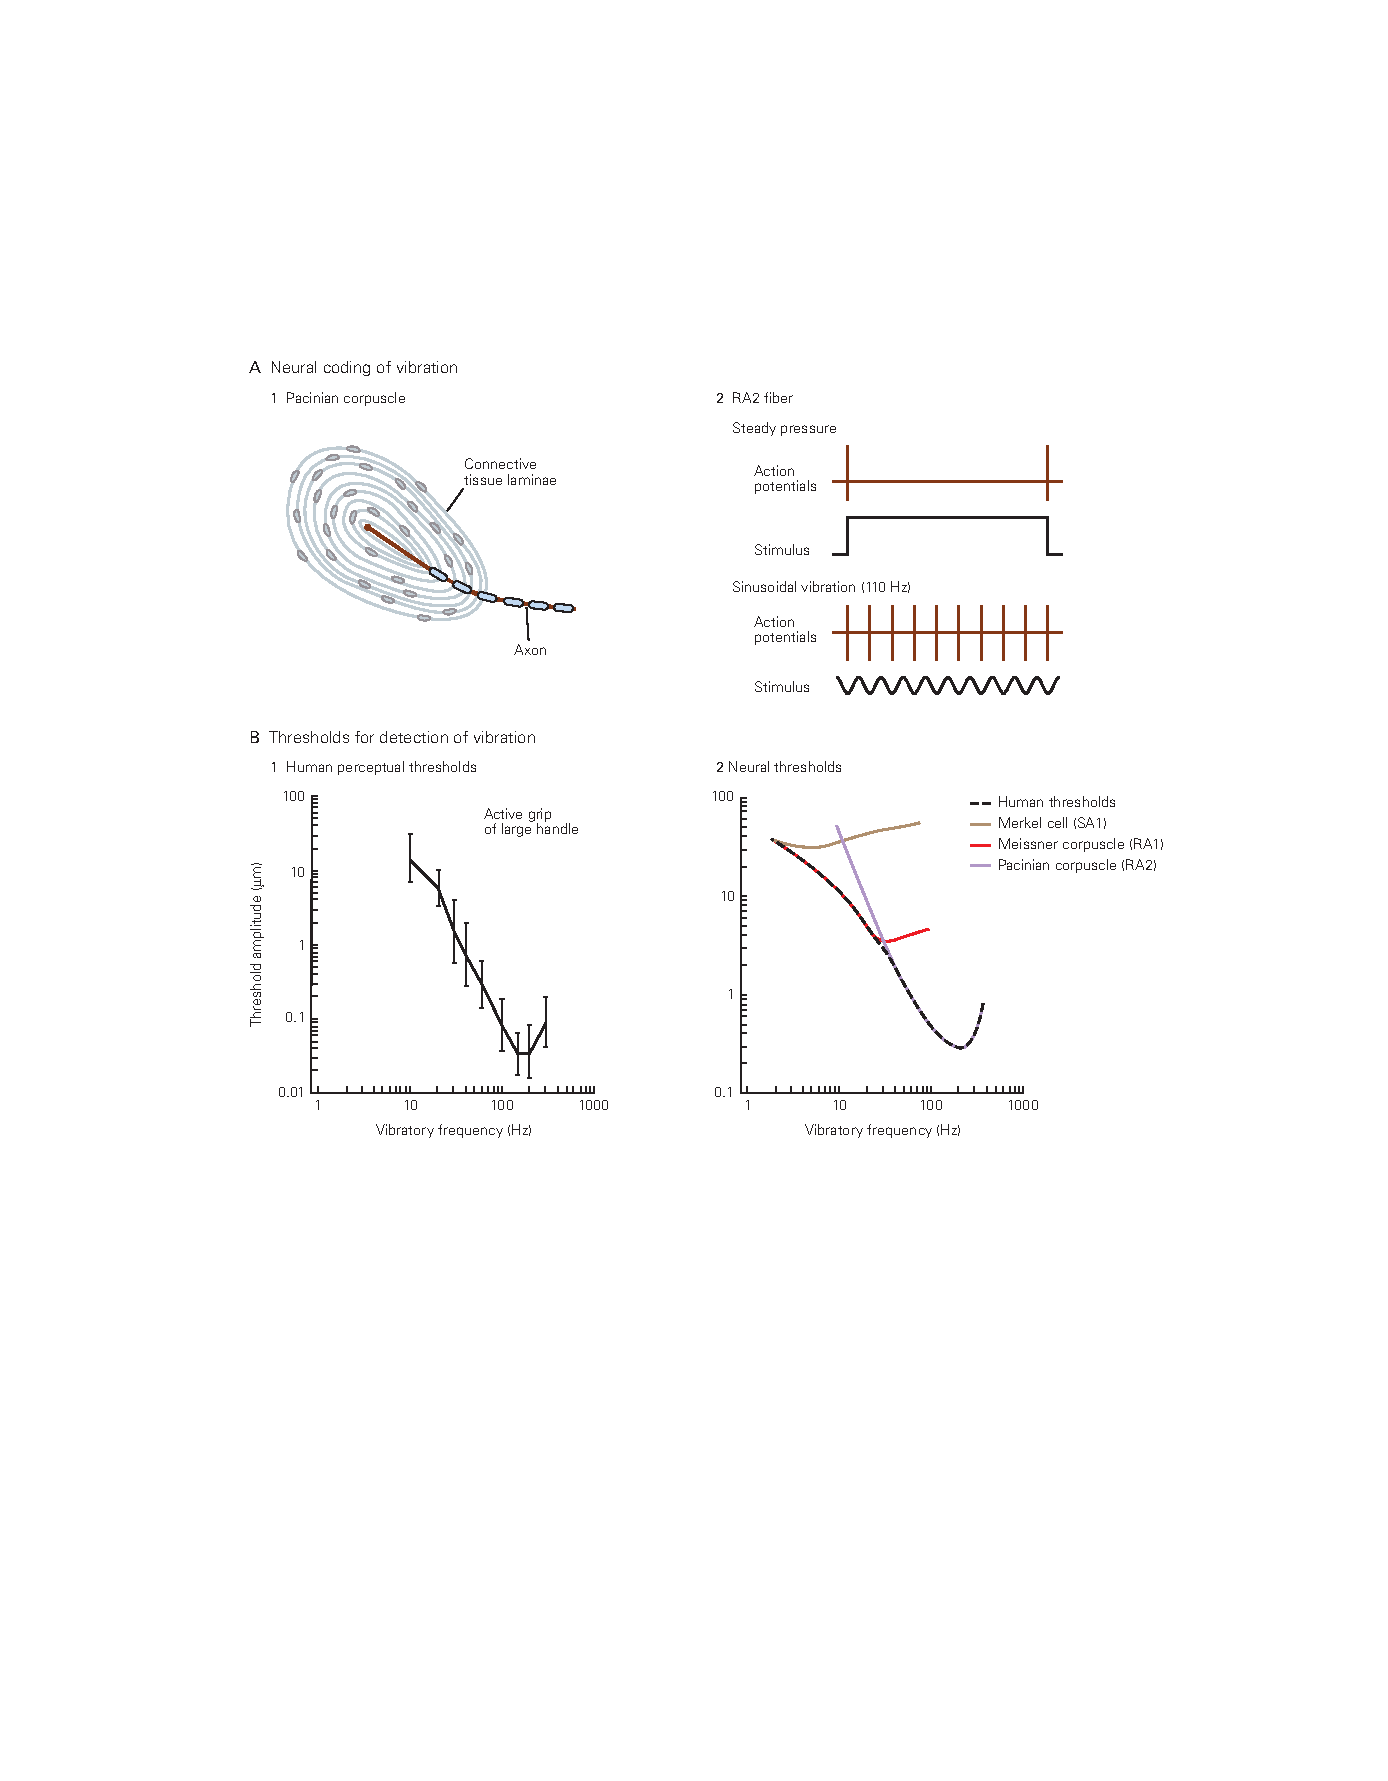
\includegraphics[width=1.0\linewidth]{chap19/fig_19_8}
	\caption{\textit{快适应2型}纤维具有最低的振动阈值。
		振动是由皮肤的正弦波刺激产生的感觉,如电动机的嗡嗡声、乐器的弦或神经系统检查中使用的音叉。
		\textbf{A.} 1. \textit{环层小体}由包裹\textit{快适应2型}纤维末端的同心、充满液体的结缔组织薄片组成。 这种结构特别适合运动检测。
		\textit{快适应2型}纤维中的感觉转导发生在与胶囊内层相连的拉伸敏感阳离子通道中。
		2. 当对皮肤施加稳定的压力时,\textit{快适应2型}纤维会在刺激开始和结束时爆发。
		作为对正弦刺激(振动)的响应,纤维会定期放电,这样每个动作电位都会发出一个刺激周期的信号。
		我们将振动视为有节奏地重复的事件,是由于同时激活许多 \textit{快适应2型}单元而产生的,这些单元同步发射\cite{talbot1968sense}。
		\textbf{B.} 1. 振动检测的心理物理阈值取决于刺激频率。
		如图所示,人类在抓取大物体时可以检测到 200 赫兹时小至 30 纳米的振动;
		阈值在其他频率和使用小探头测试时更高\cite{brisben1999detection}。
		2. 人类的振动阈值,通过压入皮肤的小探针尖端测量,与每个频率范围内最敏感的触摸纤维的阈值相匹配。 
		每种类型的机械感觉纤维对特定频率范围最敏感。
		\textit{慢适应1型}纤维是 5 赫兹以下最敏感的群体,\textit{快适应1型}纤维在 10 赫兹和 50 赫兹之间,\textit{快适应2型}纤维在 50 赫兹和 400 赫兹以上\cite{mountcastle1972detection,johansson1982responses}。}
	\label{fig:19_8}
\end{figure}



\subsection{缓慢适应的纤维检测物体压力和形状}

\textit{慢适应1型}和\textit{慢适应2型}纤维最重要的功能是它们能够发出皮肤变形和压力信号。
\textit{慢适应1型}受体对边缘、拐角、点和曲率的敏感性提供了有关物体顺应性、形状、大小和表面纹理的信息。
如果当我们触摸一个物体时它会压进皮肤,我们会认为它是硬的或坚硬的,如果我们使它变形,我们会认为它是软的。


矛盾的是,随着物体尺寸和直径的增加,其表面曲率会降低。
单个\textit{慢适应1型}纤维的反应较弱,由此产生的感觉感觉不那么明显。
例如,将铅笔尖压入皮肤 1 毫米,感觉尖锐、令人不快,并且在接触点处高度局限,而橡皮擦的 1 毫米压痕感觉又钝又宽。
最弱的感觉是由压在指垫上的平面引起的。


要理解为什么这些物体会引起不同的感觉,我们需要考虑触摸皮肤时发生的物理事件。
当铅笔尖压在皮肤上时,它会在接触点处使表面凹陷,并在周围区域(半径约 4 毫米)形成一个浅而倾斜的盆地。
虽然压痕力集中在中心,但周围区域也受到局部拉伸的扰动,称为拉伸应变。
位于皮肤中心和周围“山坡”的\textit{慢适应1型}受体受到刺激,发射与局部拉伸程度成比例的尖峰序列。


如果将第二个探针压近第一个探针,则会刺激更多的\textit{慢适应1型}纤维,但每根纤维的神经反应都会降低,因为移动皮肤所需的力由两个探针共享。
\textit{肯$\cdot$约翰逊}和他的同事已经表明,随着在感受野中添加更多的探针,每个感觉末端的反应强度会逐渐变弱,因为皮肤上的位移力分布在整个接触区。
因此,皮肤力学导致“少即是多”的情况。
单个\textit{慢适应1型}纤维对小物体的反应比对大物体的反应更强烈,因为压入皮肤所需的力集中在一个小接触点。
以这种方式,每个\textit{慢适应1型}纤维都将局部皮肤压痕轮廓整合到其接受域内。


\textit{慢适应1型}受体对皮肤局部应变的敏感性使它们能够检测到边缘,即物体曲率突然变化的地方。
当手指触摸边缘时,\textit{慢适应1型}的激活率比触摸平面时高许多倍,因为物体边界施加的力使皮肤不对称地移位,超出边缘以及在边缘处。
这种力的不对称分布增强了位于物体边缘的感受野的响应。
由于边缘通常被认为是锋利的,我们倾向于在平坦或轻微弯曲的表面上而不是通过边缘来抓住物体。


支配\textit{鲁菲尼终末器}的\textit{慢适应2型}纤维对皮肤拉伸的反应比对压痕的反应更强烈,因为它们的解剖学位置沿着手掌皱襞或手指关节。
它们提供有关用整只手抓住大物体形状的信息,即物体被压在手掌上的“力量抓握”。


\textit{慢适应2型}系统可能在立体视觉(仅使用触摸来识别三维物体)以及其他以皮肤拉伸为主要线索的感知任务中发挥核心作用。
\textit{贝诺尼$\cdot$爱丁}表明,手背毛茸茸的皮肤的\textit{慢适应2型}神经支配在手形和手指位置的感知中起着重要作用。
\textit{慢适应2型}纤维通过检测指关节或手指之间的织带中的皮肤拉伸来帮助感知手指关节角度。
这些关节附近的\textit{鲁菲尼终末器}对齐,以便在手指向特定方向移动时刺激不同的感受器组(图~\ref{fig:19_5}A,底部面板)。
以这种方式,\textit{慢适应2型}系统提供了整个手部皮肤伸展的神经表征,一种本体感受而非外感受功能。


当手空着时,\textit{慢适应2型}纤维还提供有关手形和手指运动的本体感受信息。
如果手指完全伸展和外展,我们会感觉到手掌和近端指骨的拉伸,因为无毛的皮肤变平了。
同样,如果手指完全弯曲并握拳,我们会感觉到手背皮肤的拉伸,尤其是掌指关节和近端指间关节。
人类使用这种本体感受信息来预先塑造他们的手以有效地抓住物体,将手指张开到足以清除物体并熟练地抓住它而不用太大力。



\subsection{快适应纤维检测运动和振动}

振动觉测试是神经学检查的重要组成部分。
用以特定频率振荡的音叉触摸皮肤会引起周期性的嗡嗡声,因为大多数触觉感受器会同步发射与刺激频率同相的周期性动作电位序列(图~\ref{fig:19_8}A2)。
振动感是对触摸的动态敏感度的有用测量,特别是在局部神经损伤的情况下。


\textit{快适应2型}受体,即\textit{环层小体},是体感系统中最敏感的机械感受器。
它对高频(30-500 赫兹)振动刺激反应灵敏,可以检测纳米范围内 250 赫兹的振动(图~\ref{fig:19_8}B2)。
\textit{环层小体}过滤和放大高频振动的能力使我们能够感觉到手中工具工作表面的状况,就好像我们的手指本身正在触摸工具下的物体一样。
临床医生利用这种敏锐的灵敏度将针头引导到血管中并探测组织硬度。
汽车修理工使用振动感将扳手定位在看不见的螺栓上。
我们可以在黑暗中书写,因为我们能感觉到钢笔接触纸张时的振动,并将摩擦力从表面粗糙度传递到我们的手指。


尽管\textit{环层小体}对于大于 40 赫兹的频率具有最低的振动阈值(图~\ref{fig:19_8}B2),更高振幅的振动刺激也会激发\textit{慢适应1型}和\textit{快适应1型}纤维,即使它们诱发的尖峰序列比\textit{环层小体}传入神经弱。
图\ref{fig:19_9}A 说明了 15 种不同周围神经纤维在 20 赫兹下以弱、中等和高振幅刺激的诱发放电模式。
尽管这些纤维对振动的敏感度不同,但它们的尖峰序列具有某些重要的共同特征。
首先,每个神经元在振动周期的特定阶段放电,通常是当探头压入皮肤时,其尖峰相位模式复制振动频率:
当以 20 赫兹刺激时,尖峰脉冲以大约 50 毫秒的间隔重复出现。
尖峰序列的模式得到进一步加强,因为纤维群同步发射,使频率信息能够由于突触整合而集中保存。


\begin{figure}[htbp]
	\centering
	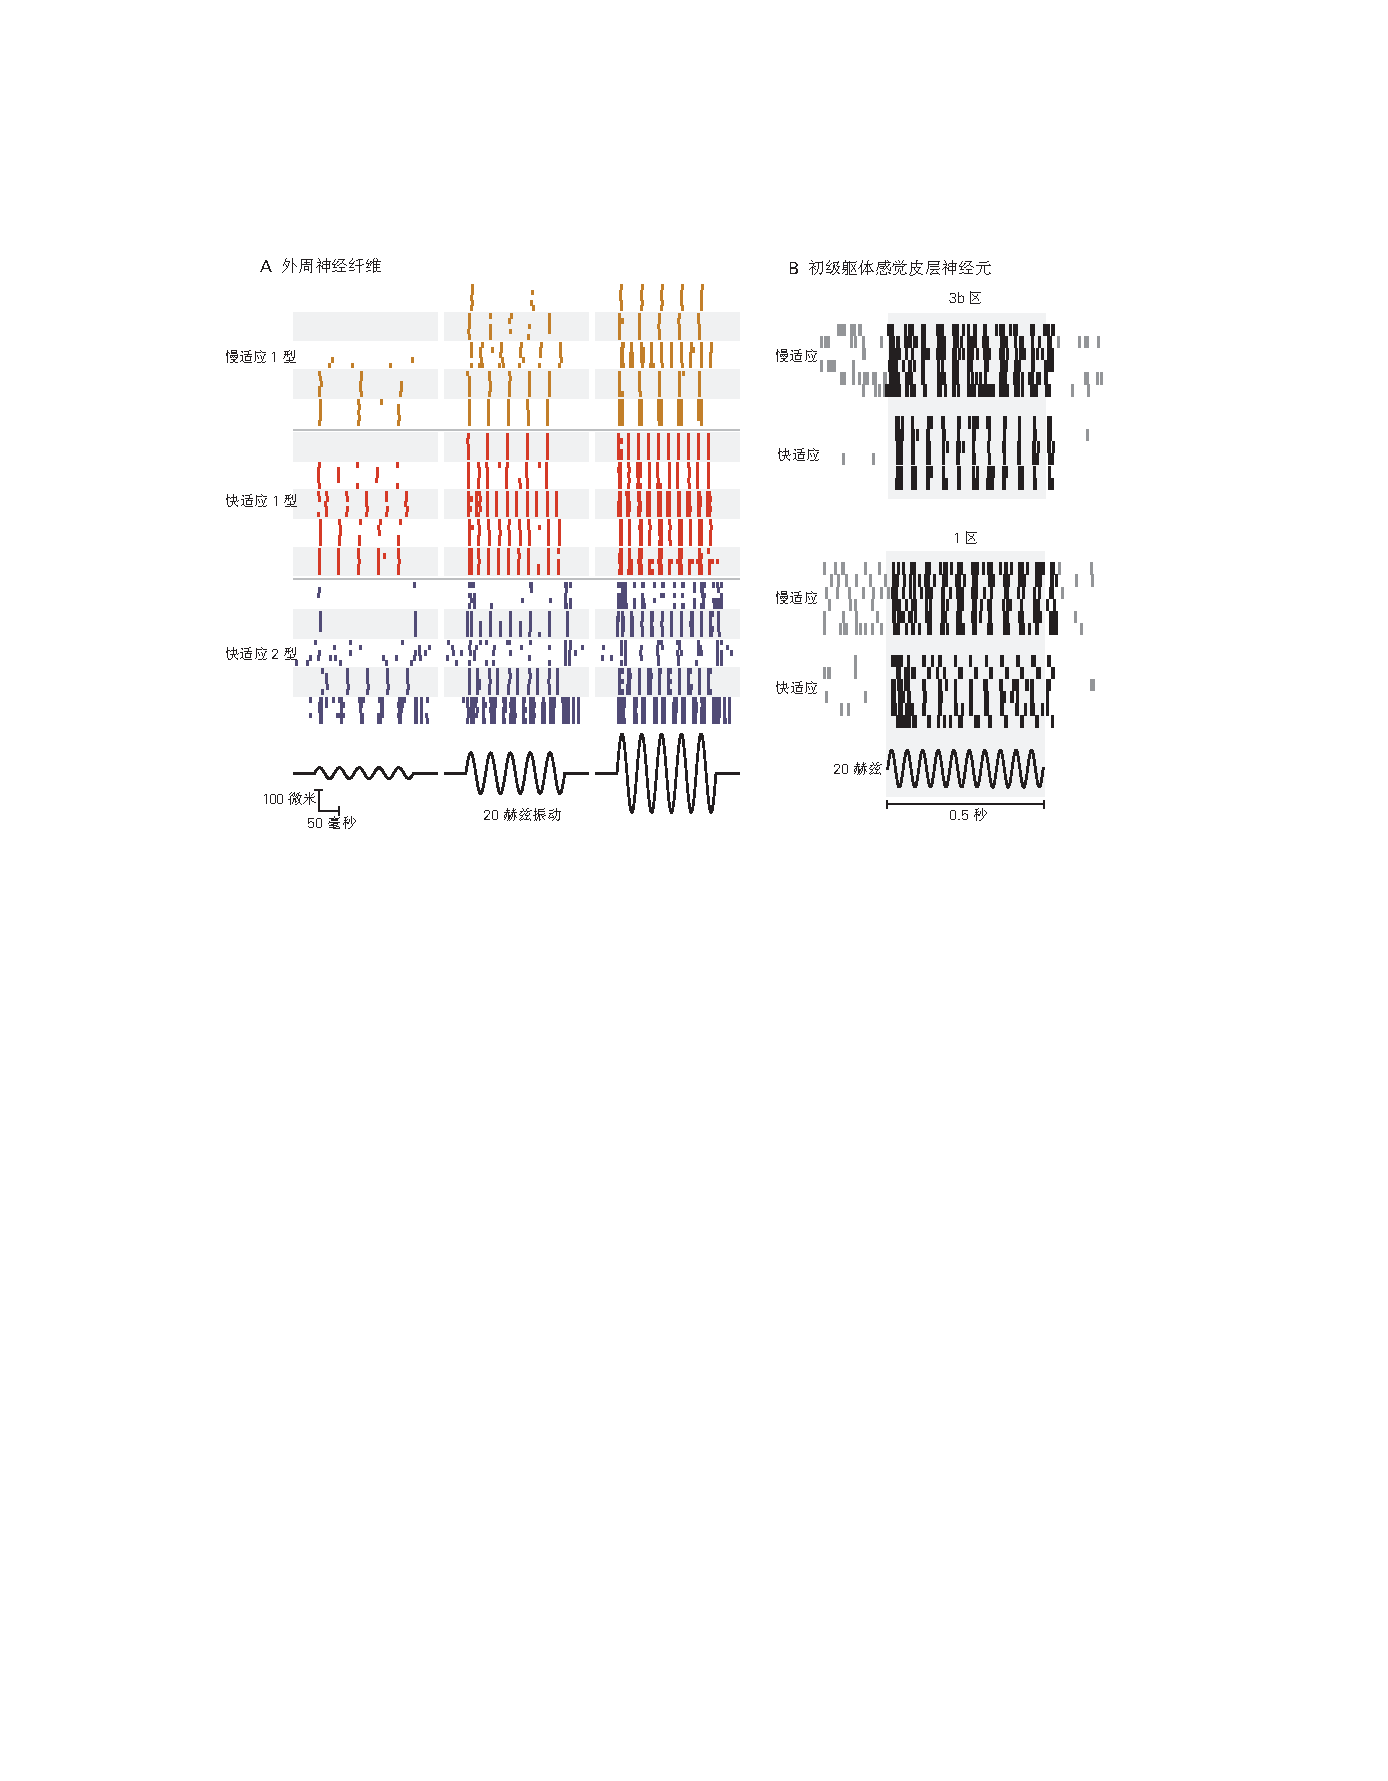
\includegraphics[width=1.0\linewidth]{chap19/fig_19_9}
	\caption{超阈值振动激活多类触觉感受器。 
		\textbf{A.} 从猕猴的 15 种不同体感纤维中记录的尖峰序列的光栅,这些体感纤维受到振幅为 35(左)、130(中)和 250 微米(右)的 20 赫兹振动刺激的刺激。
		交替的阴影和白色带表示个体\textit{慢适应1型}、\textit{快适应1型}和\textit{快适应2型}触摸纤维对同一刺激的五次呈现的反应。
		神经反应被分组为一个或多个尖峰的爆发,这些尖峰与每个振动周期的压痕阶段同步发生。
		每根纤维中每个周期的尖峰总数与振动幅度相关; 这个群体发射的尖峰总数也反映了振动幅度。
		尽管单个神经元的反应强度不同,但每条触摸纤维的尖峰序列在每次试验中都非常相似,并且在神经元之间同步发生\cite{muniak2007neural}。
		\textbf{B.} \textit{初级躯体感觉皮层}对 20 赫兹振动的反应。
		猕猴\textit{初级躯体感觉皮层}区域 3b(顶部)的两个神经元和区域 1(底部)的两个神经元中诱发的尖峰序列光栅。
		阴影区域表示振动刺激的周期。
		与周围神经一样,\textit{初级躯体感觉皮层}神经元对低频振动作出反应,脉冲群与刺激率同相。
		请注意,脉冲序列因试验而异,并且在区域 1 中的周期性低于区域 3b 中的周期性。
		与\textit{初级躯体感觉皮层}相比,\textit{次级躯体感觉皮层}皮层(参见图~\ref{fig:19_21})的放电周期甚至更不明显\cite{salinas2000periodicity}。}
	\label{fig:19_9}
\end{figure}


随着刺激幅度的增加,每次爆发的尖峰总数也增加,允许每根纤维多路复用振动频率和强度的信号:
频率信息由尖峰序列的时间模式传达,振动幅度由总编码 每根纤维每秒发射的尖峰数,以及激活纤维集合的总尖峰输出。
最后,请注意,每个神经元的尖峰序列在时间过程中非常相似,并且每个条件下每次试验的尖峰计数都非常相似,这表明触觉传入纤维提供的感觉信号具有很高的可靠性。 
感觉编码的这种可靠性和可预测性使振动成为评估触觉的一种特别有用的技术。



\subsection{慢适应和快适应的纤维对握力控制都很重要}

除了感知物体的物理特性外,触觉感受器还提供有关熟练动作中手部动作的重要信息。
\textit{罗兰$\cdot$约翰逊}和\textit{格伦$\cdot$韦斯特林}使用显微神经造影术来确定当物体被抓在手中时触觉感受器的作用。
通过将微电极放置在正中神经中,他们能够记录触摸纤维在手指最初接触物体时的放电模式,以及当物体被拇指和食指抓住、举起、放在桌子上方、放低、 并返回休息。


他们发现所有四类触摸纤维都对抓握有反应,并且每种纤维类型都监控特定功能。
在没有触觉刺激的情况下,\textit{快适应1型}、\textit{快适应2型}和\textit{慢适应1型}纤维通常是沉默的。
当物体第一次被触摸时,它们会检测到接触(图~\ref{fig:19_10})。
\textit{慢适应1型}纤维发出每个手指施加的握力大小的信号,\textit{快适应1型}纤维感知施加抓握的速度。
\textit{快适应2型}纤维检测从桌子上提起和返回时通过物体传输的小冲击波。
我们知道物体何时由于这些振动而与桌面接触,因此可以在不看物体的情况下操纵物体。
\textit{快适应1型}和\textit{快适应2型}纤维在掌握建立后停止响应。
\textit{慢适应2型}纤维在抓取或释放物体期间发出手指弯曲或伸展的信号,从而在这些运动进行时监测手部姿势。


\begin{figure}[htbp]
	\centering
	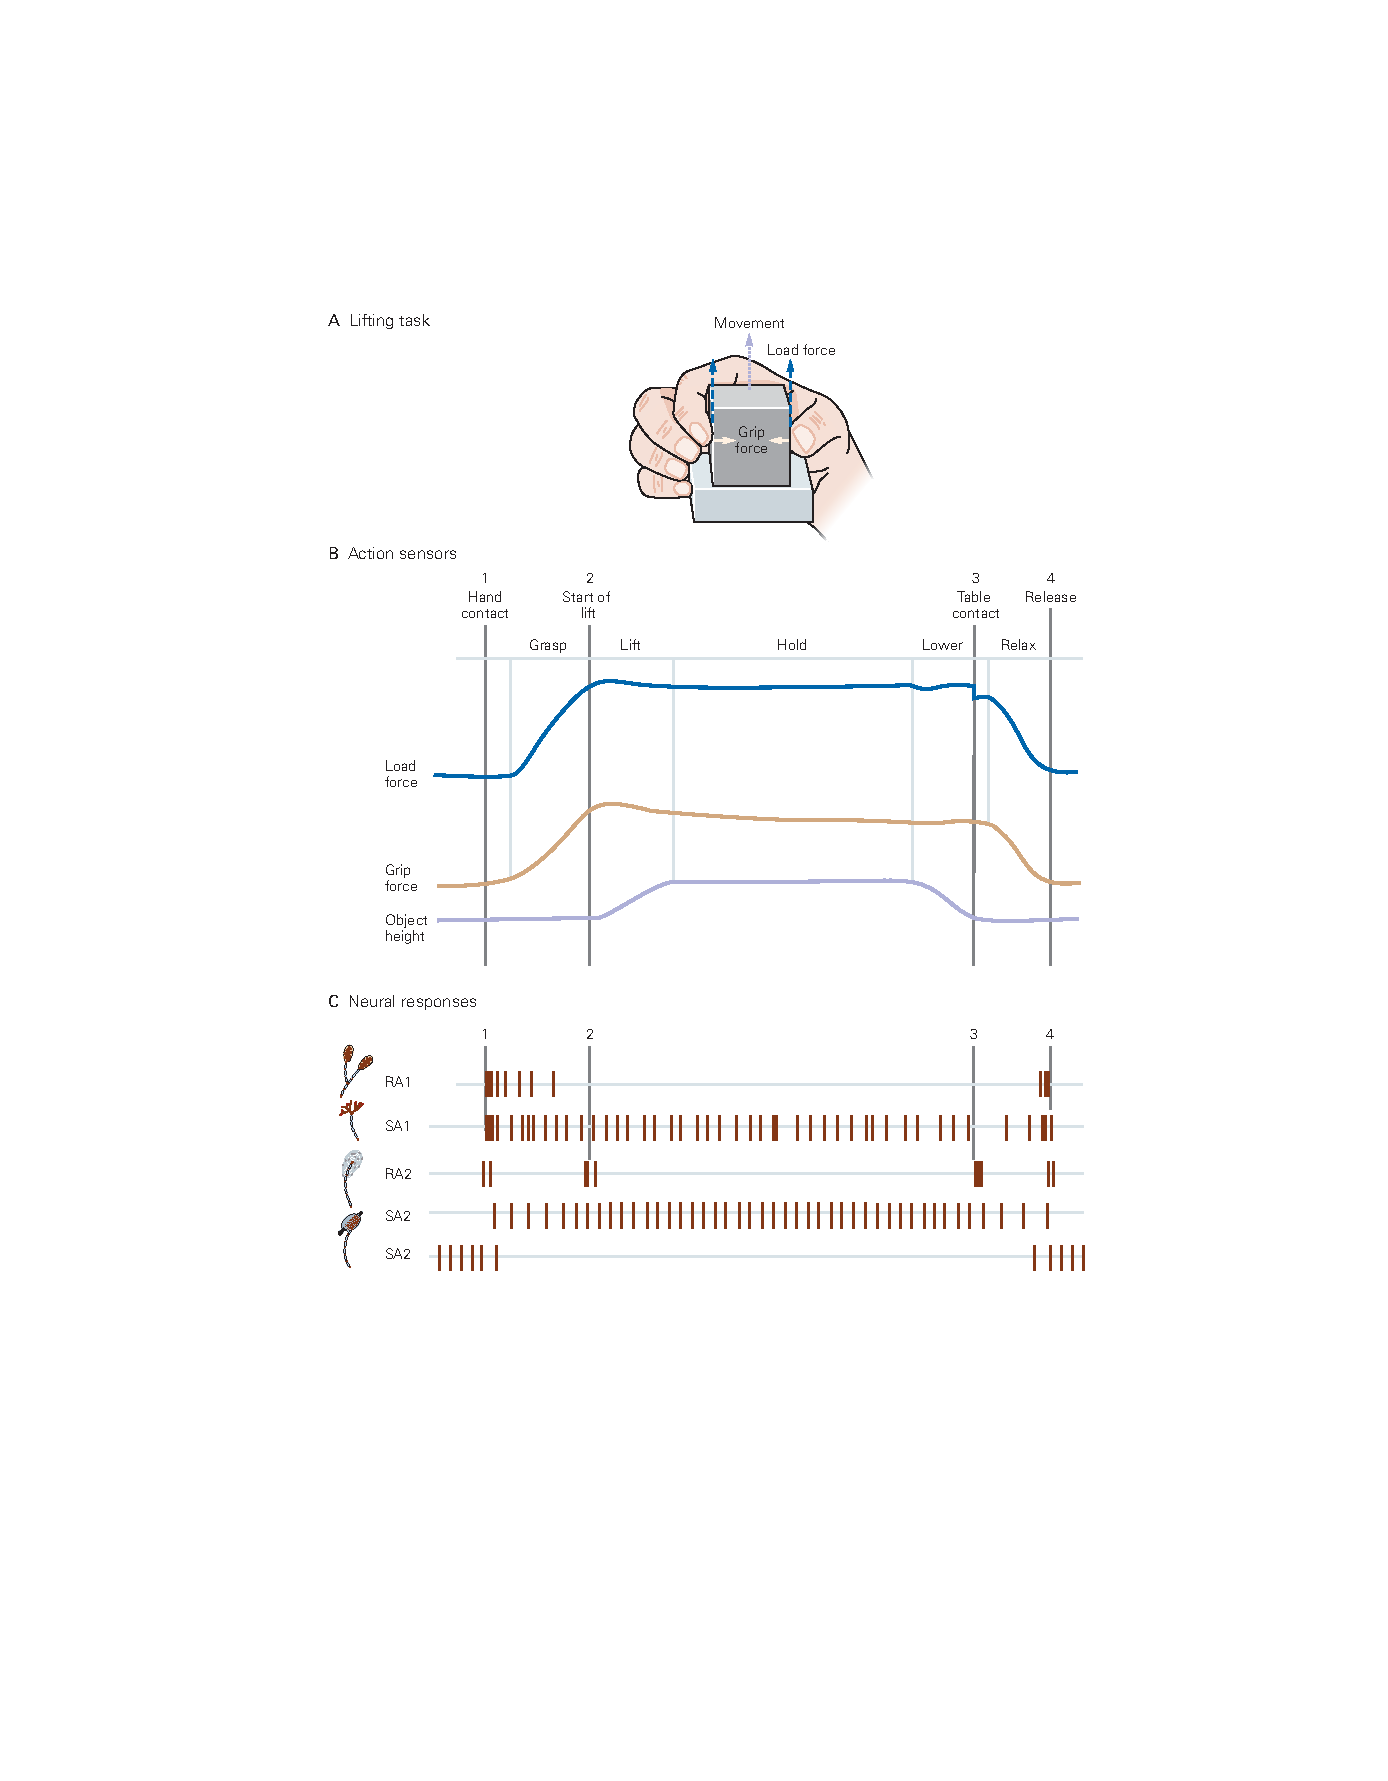
\includegraphics[width=1.0\linewidth]{chap19/fig_19_10}
	\caption{在抓取和举起过程中来自手的感觉信息\cite{johansson1996sensory}。
		\textbf{A.} 受试者在拇指和指尖之间抓住并提起一块木块,将其放在桌子上方,然后将其放回静止位置。
		法向(抓握)力将物体固定在手中,切向(负载)力克服重力。
		握力适应物体的表面纹理和重量。
		\textbf{B.} 夹持力和负载力由物体中的传感器监控。
		这些力在与物体接触后协调,在升力开始时稳定,并在物体返回到桌子后一致放松。
		\textbf{C.} 所有四个机械感受器都检测到手与物体的接触,但随着任务的进行,每个都监测动作的不同方面。
		\textit{慢适应1型}纤维编码握力,\textit{慢适应2型}纤维编码手部姿势。
		\textit{快适应1型}纤维对手在物体上施加力和移动的速率进行编码。
		\textit{快适应2型}纤维在每个任务阶段感知物体的振动:
		手部接触、抬起、桌面接触和松开抓握。}
	\label{fig:19_10}
\end{figure}


来自手的报告物体形状、大小和质地的信号是控制抓取过程中力应用的重要因素。
\textit{约翰逊}和他的同事发现,我们举起和操纵物体时非常灵敏(握力刚好超过导致明显滑动的力),并且握力会自动调整以补偿手指和物体表面之间摩擦系数的差异。
受试者预测抓住和举起物体需要多大的力,并根据\textit{慢适应1型}和\textit{快适应1型}传入神经提供的触觉信息修改这些力。
具有光滑表面的物体比具有粗糙纹理的物体更牢固地抓住,在手与物体的初始接触期间由\textit{快适应1型}传入编码的属性。
在神经损伤或手部局部麻醉期间,可以看到触觉信息在抓握中的重要性;
患者施加异常高的握力,手指施加的握力和负载力之间的协调性很差。


\textit{快适应1型}受体提供的用于监测抓握动作的信息对于抓握控制至关重要,它使我们能够在扰动导致物体意外滑落时抓住物体。
\textit{快适应1型}纤维在稳定抓握过程中保持安静,并且通常保持安静,直到物体恢复静止并释放抓握。
然而,如果物体出乎意料地重或被外力摇晃并开始从手中滑落,\textit{快适应1型}纤维会响应物体的小切向滑动运动而激发。 
\textit{快适应1型}活动的最终结果是来自运动皮层的信号增加了握力。



\section{触觉信息在中央触摸系统中处理}

支配手的感觉传入纤维通过正中神经、尺神经和浅表桡神经将触觉和其他体感信息传递到中枢神经系统。
这些神经同侧终止于 C6 至 T1 脊柱节段;
这些纤维的其他分支通过同侧背柱直接投射到髓质,在那里它们与楔形核中的神经元建立突触连接,楔形核是背柱核的外侧分裂(图~\ref{fig:19_11})。


\begin{figure}[htbp]
	\centering
	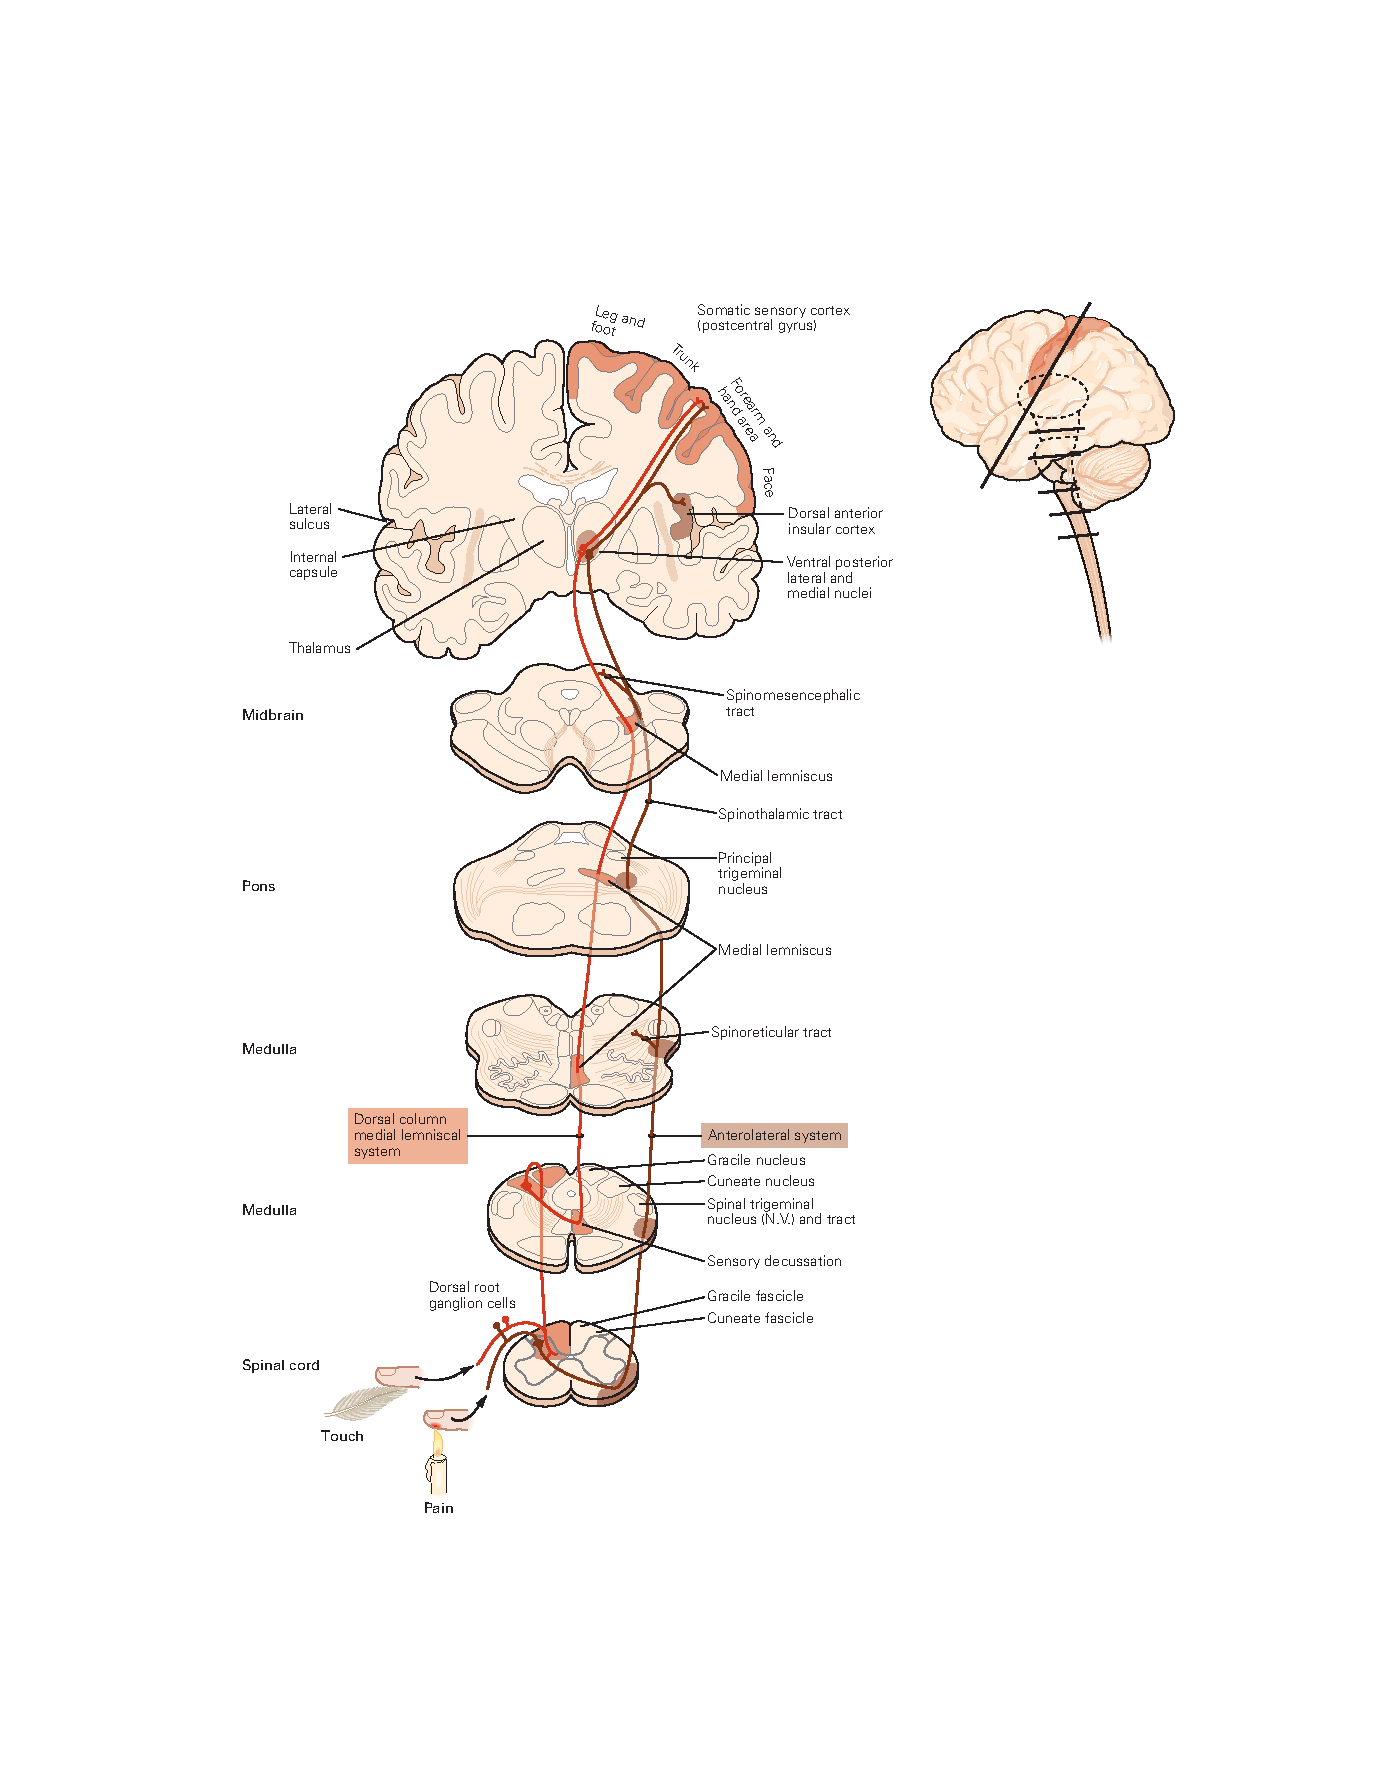
\includegraphics[width=1.0\linewidth]{chap19/fig_19_11}
	\caption{来自四肢和躯干的体感信息通过两条上行通路传递到\textit{丘脑}和大脑皮层。
		沿着从脊髓到大脑的神经轴的脑切片说明了将体感信息传递到大脑皮层的两条主要通路的解剖结构。
		这两条通路在到达\textit{脑桥之前}是\textit{分开}的,它们在那里并列。
		背柱,即内侧丘系系统(橙色)。
		触摸和肢体本体感觉信号通过大直径有髓神经纤维传递到脊髓和脑干,并在该系统中传递到丘脑。
		在脊髓中,用于触觉和本体感觉的纤维分开,一个分支进入同侧脊髓灰质,另一个在同侧背柱中上升到髓质。 
		来自背柱核神经元的二级纤维在髓质中穿过中线并在对侧内侧丘系中上升至丘脑,在那里它们终止于外侧和内侧腹侧后核。
		这些核中的丘脑神经元将触觉和本体感受信息传递给初级体感皮层。 前外侧系统(棕色)。
		疼痛、瘙痒、温度和内脏信息通过终止于同侧背角的小直径有髓和无髓纤维传递到脊髓。
		该信息由脊髓内的神经元通过中线传递,并传递到对侧前外侧系统中的脑干和丘脑。
		终止于脑干的前外侧纤维组成脊髓网状束和脊髓中脑束; 剩余的前外侧纤维形成脊髓丘脑束。}
	\label{fig:19_11}
\end{figure}



\subsection{脊髓、脑干和丘脑回路分离触觉和本体感觉}

背柱中的纤维和背柱核中的神经元按地形图组织,上半身(包括手)在楔形束和核的外侧表示,下半身在细束和核的内侧表示。
触觉和本体感觉的体感子模态在这些区域中也在功能上分离,因为单个脊髓和脑干神经元从单一类型的传入神经元接收突触输入,而不同类型的神经元在空间上是分离的。 
背柱核的头侧三分之一由处理来自肌肉传入神经的本体感受信息的神经元控制; 触觉输入在尾部更占主导地位。
模态隔离是投射到初级体感皮层的通路的一贯特征。


背柱核中的神经元将其轴突投射到延髓的中线,形成内侧丘系,这是一种突出的纤维束,可将触觉和本体感受信息从身体的对侧通过脑桥和中脑传递到丘脑。
由于感觉纤维的这种交叉(或交叉),大脑的左侧从身体右侧的机械感受器接收体感输入,反之亦然。
在运输过程中,身体在内侧丘系和丘脑内的躯体表征变得颠倒;
身体的地形图在中间显示面部,在侧面显示下半身,在中间显示上半身和手。


来自手和身体其他区域的触觉和本体感受信息在丘脑的不同亚核中进行处理。
来自四肢和躯干的触摸信号通过内侧丘系被发送到\textit{腹后外侧}核,而来自面部和嘴巴的触摸信号被传送到\textit{腹后内侧}核。
来自肌肉和关节(包括手部)的本体感受信息被传输到\textit{腹后上}核。
这些核将它们的输出发送到大脑皮层顶叶的不同子区域。 
\textit{腹后外侧}核和\textit{腹后内侧}核主要将皮肤信息传递到\textit{初级躯体感觉皮层}的 3b 区,而\textit{腹后上}核主要将本体感受信息传递到 3a 区。



\subsection{体感皮层被组织成功能专门的柱}

有意识的触觉意识被认为起源于大脑皮层。
触觉信息通过位于顶叶中央后回的\textit{初级躯体感觉皮层}进入大脑皮层。
初级躯体感觉皮层包括四个细胞结构区域:布罗德曼区域 3a、3b、1 和 2(图~\ref{fig:19_12})。
这些区域相互关联,因此\textit{初级躯体感觉皮层}中的感官信息处理涉及串行和并行处理。


\begin{figure}[htbp]
	\centering
	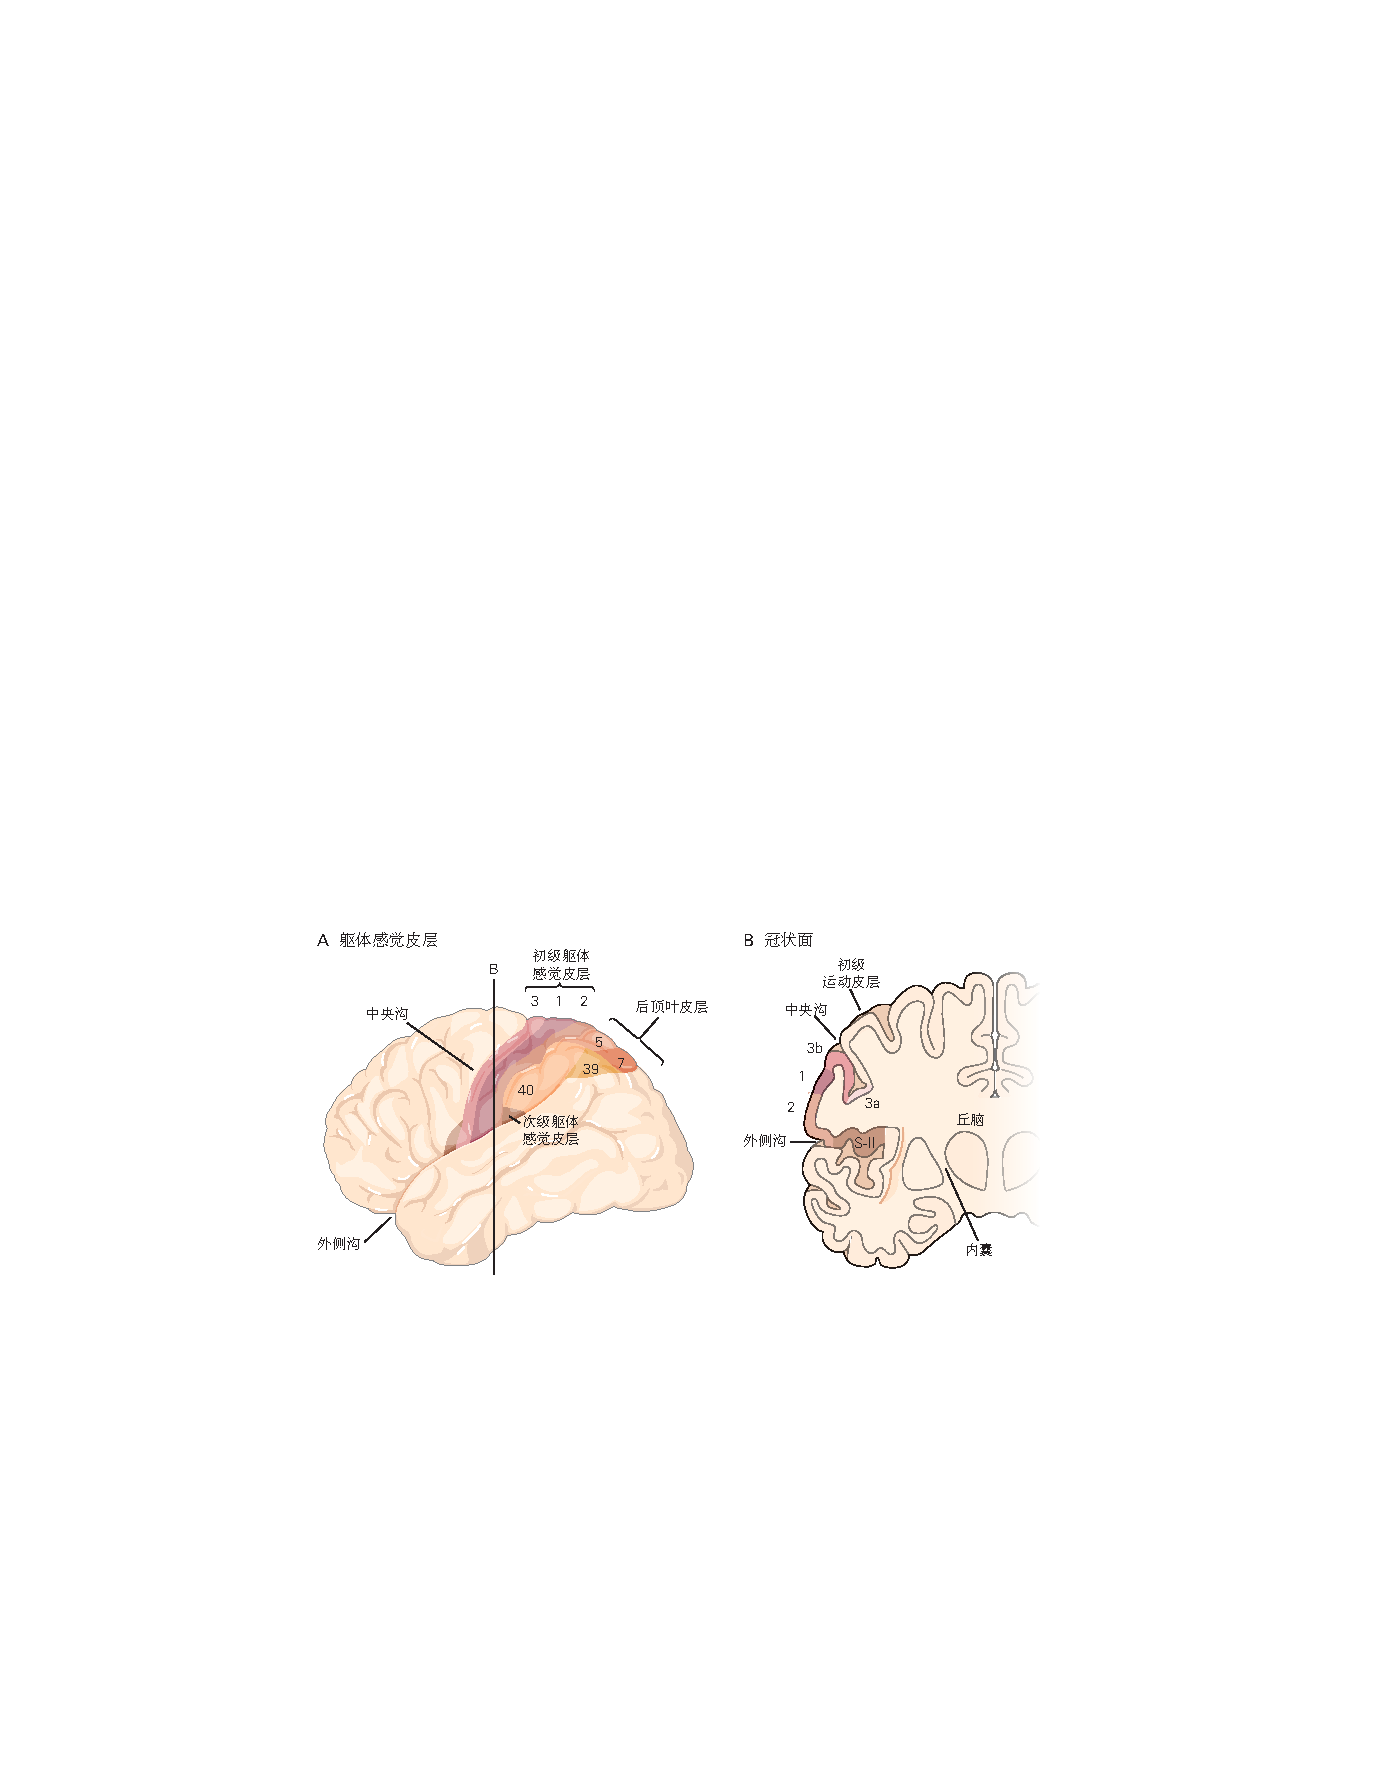
\includegraphics[width=1.0\linewidth]{chap19/fig_19_12}
	\caption{人脑中大脑皮层的体感区。
		\textbf{A.} 皮层的体感区域位于顶叶,由三个主要部分组成。
		\textit{初级躯体感觉皮层}形成顶叶的前部。
		它从中央沟底部开始延伸到整个中央后回,向后延伸至中央后沟,并进入半球内侧壁至扣带回(未显示)。
		\textit{初级躯体感觉皮层}皮层包括四个不同的细胞构造区域:\textit{布罗德曼} 3a、3b、1 和 2 区。
		\textit{次级躯体感觉皮层}位于外侧沟(外侧裂)上岸和顶叶盖上;
		它覆盖\textit{布罗德曼} 43 区。
		后顶叶皮层围绕半球外侧表面的顶内沟,从中央后沟延伸至顶枕沟,并在内侧延伸至楔前叶。
		上顶叶小叶(\textit{布罗德曼}  5 和 7 区)是一个体感区;
		下顶叶小叶(区域 39 和 40)接收体感和视觉输入。
		\textbf{B.} 中央后回的冠状切面说明了\textit{初级躯体感觉皮层}、\textit{次级躯体感觉皮层}和初级运动皮层(区域 4)的解剖关系。
		\textit{次级躯体感觉皮层}与\textit{初级躯体感觉皮层}中的区域 2 相邻,并沿着外侧沟的上岸向内侧延伸至岛叶皮层。
		初级运动皮层位于中央沟前壁内 3a 区的嘴侧。}
	\label{fig:19_12}
\end{figure}


在对大脑皮层的一系列开创性研究中,\textit{弗农$\cdot$芒卡斯尔}发现\textit{初级躯体感觉皮层}皮层被组织成垂直的柱状或板状结构。
每列宽 300 至 600 微米,横跨从软脑膜表面到白质的所有六个皮层(图~\ref{fig:19_13})。
列内的神经元接收来自同一局部皮肤区域的输入,并对同一类或多类触觉感受器做出反应。
因此,纵柱包含新皮层的基本功能模块;
它提供了一个解剖结构,组织感官输入以传达有关位置和形态的相关信息。


\begin{figure}[htbp]
	\centering
	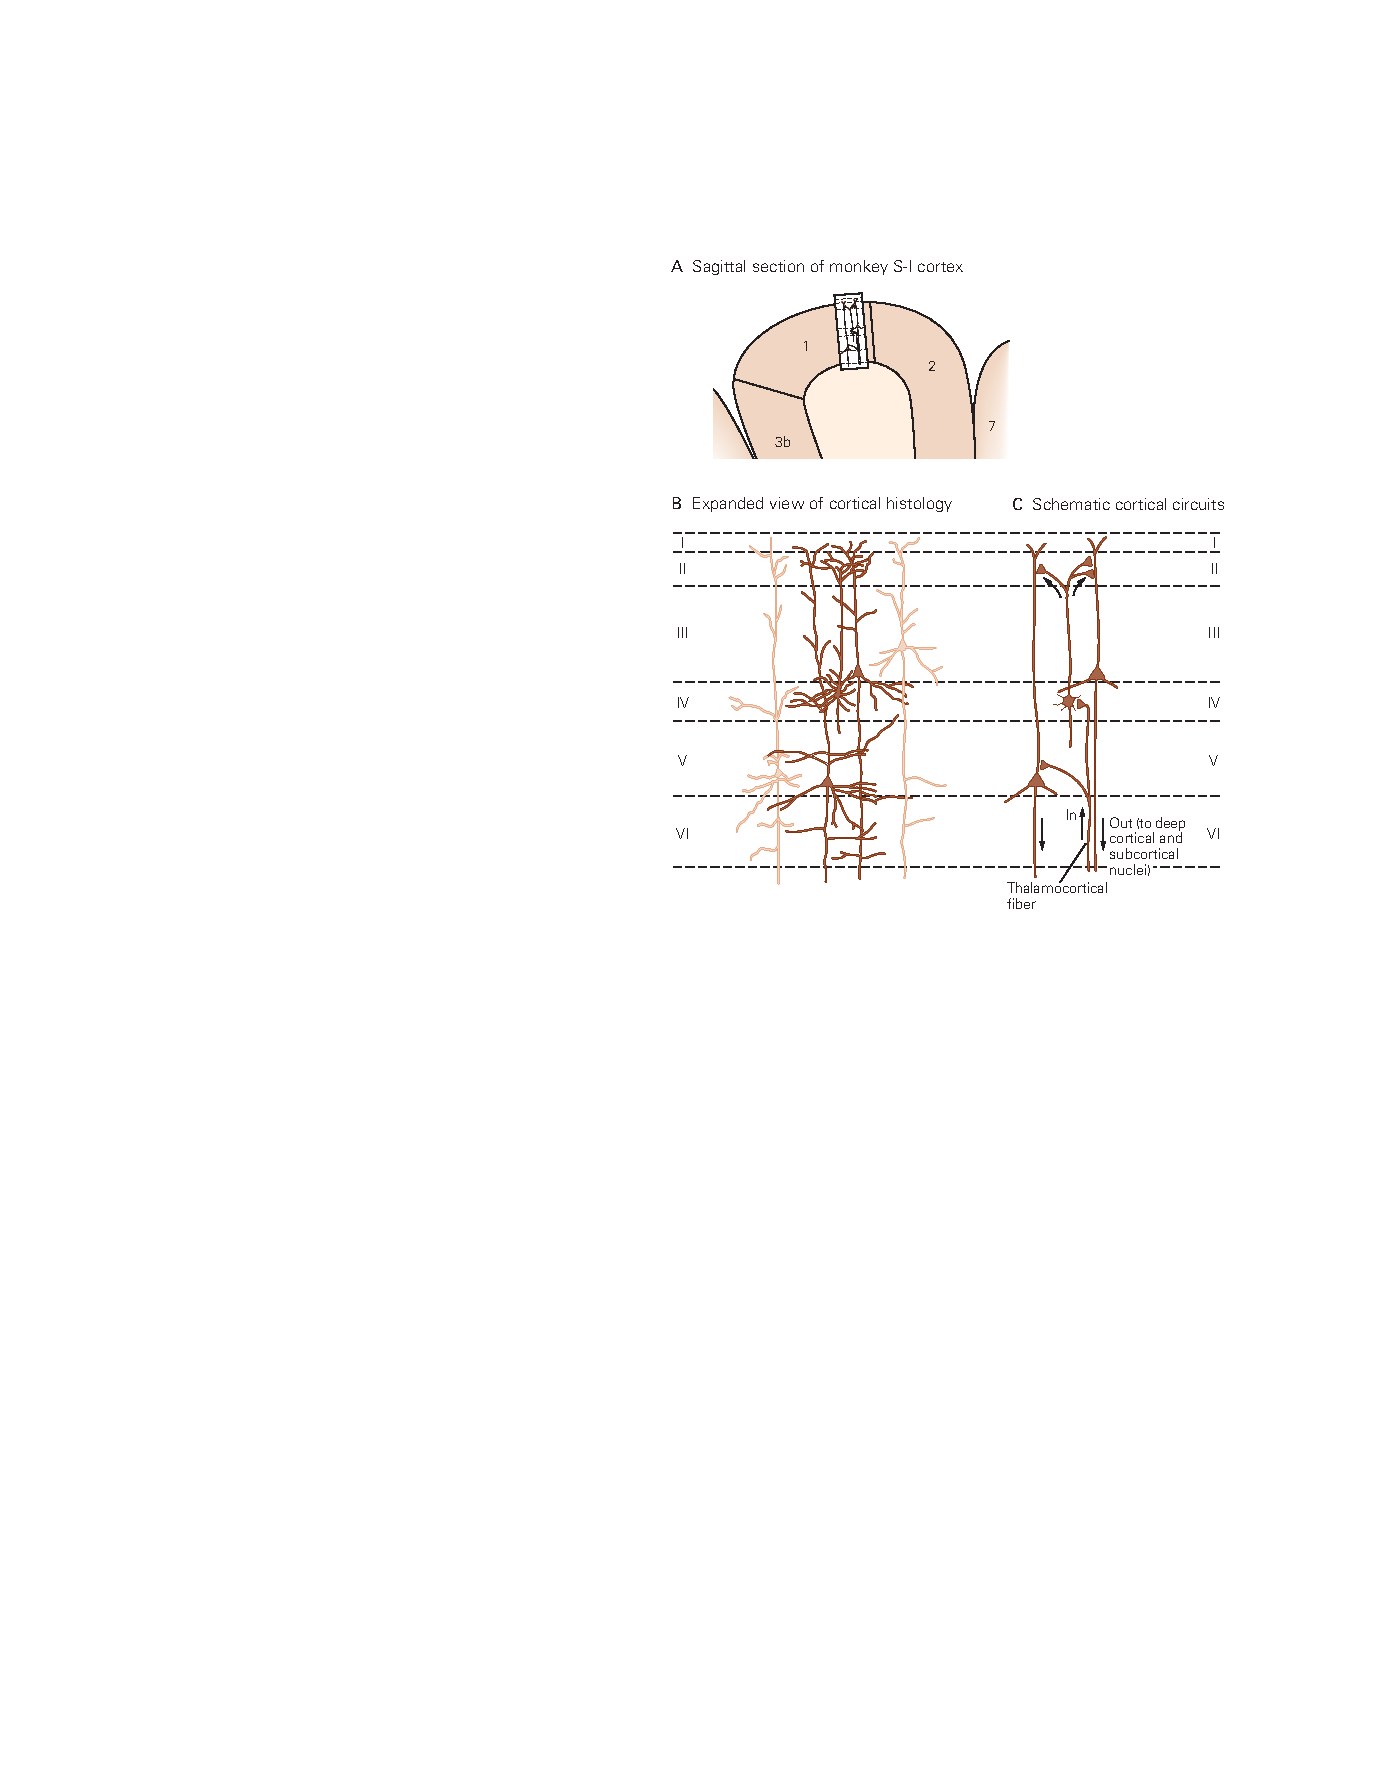
\includegraphics[width=0.75\linewidth]{chap19/fig_19_13}
	\caption{躯体感觉皮层柱内神经回路的组织。
		来自皮肤或深层组织的感觉输入被组织成从大脑表面延伸到白质的神经元柱。
		每一列主要在第四层接收来自身体一部分的丘脑输入。
		IV 层中的兴奋性神经元将其轴突垂直送向皮层表面,接触 II 层和 III 层(颗粒上层)中锥体神经元的树突以及颗粒下层(V 层和 VI 层)中锥体细胞的顶端树突。
		以这种方式,来自身体部位(例如手指)的触觉信息垂直分布在一列神经元内。}
	\label{fig:19_13}
\end{figure}


皮层的柱状组织是内在皮层回路、丘脑皮层轴突的投射模式和皮层发育过程中成神经细胞迁移途径的直接结果。
列内的连接模式垂直定向,垂直于皮层表面。
丘脑皮层轴突主要终止于第 IV 层的星状细胞簇,其轴突垂直投射到皮层表面,以及星形金字塔细胞。
因此,丘脑皮层输入被中继到锥体细胞的窄列,这些细胞与第 IV 层细胞轴突接触。
其他皮层中皮层锥体细胞的顶端树突和轴突也主要垂直定向,平行于丘脑皮质轴突和星状细胞轴突(图~\ref{fig:19_14})。
这使得相同的信息可以由整个皮层厚度的一列神经元处理。


\begin{figure}[htbp]
	\centering
	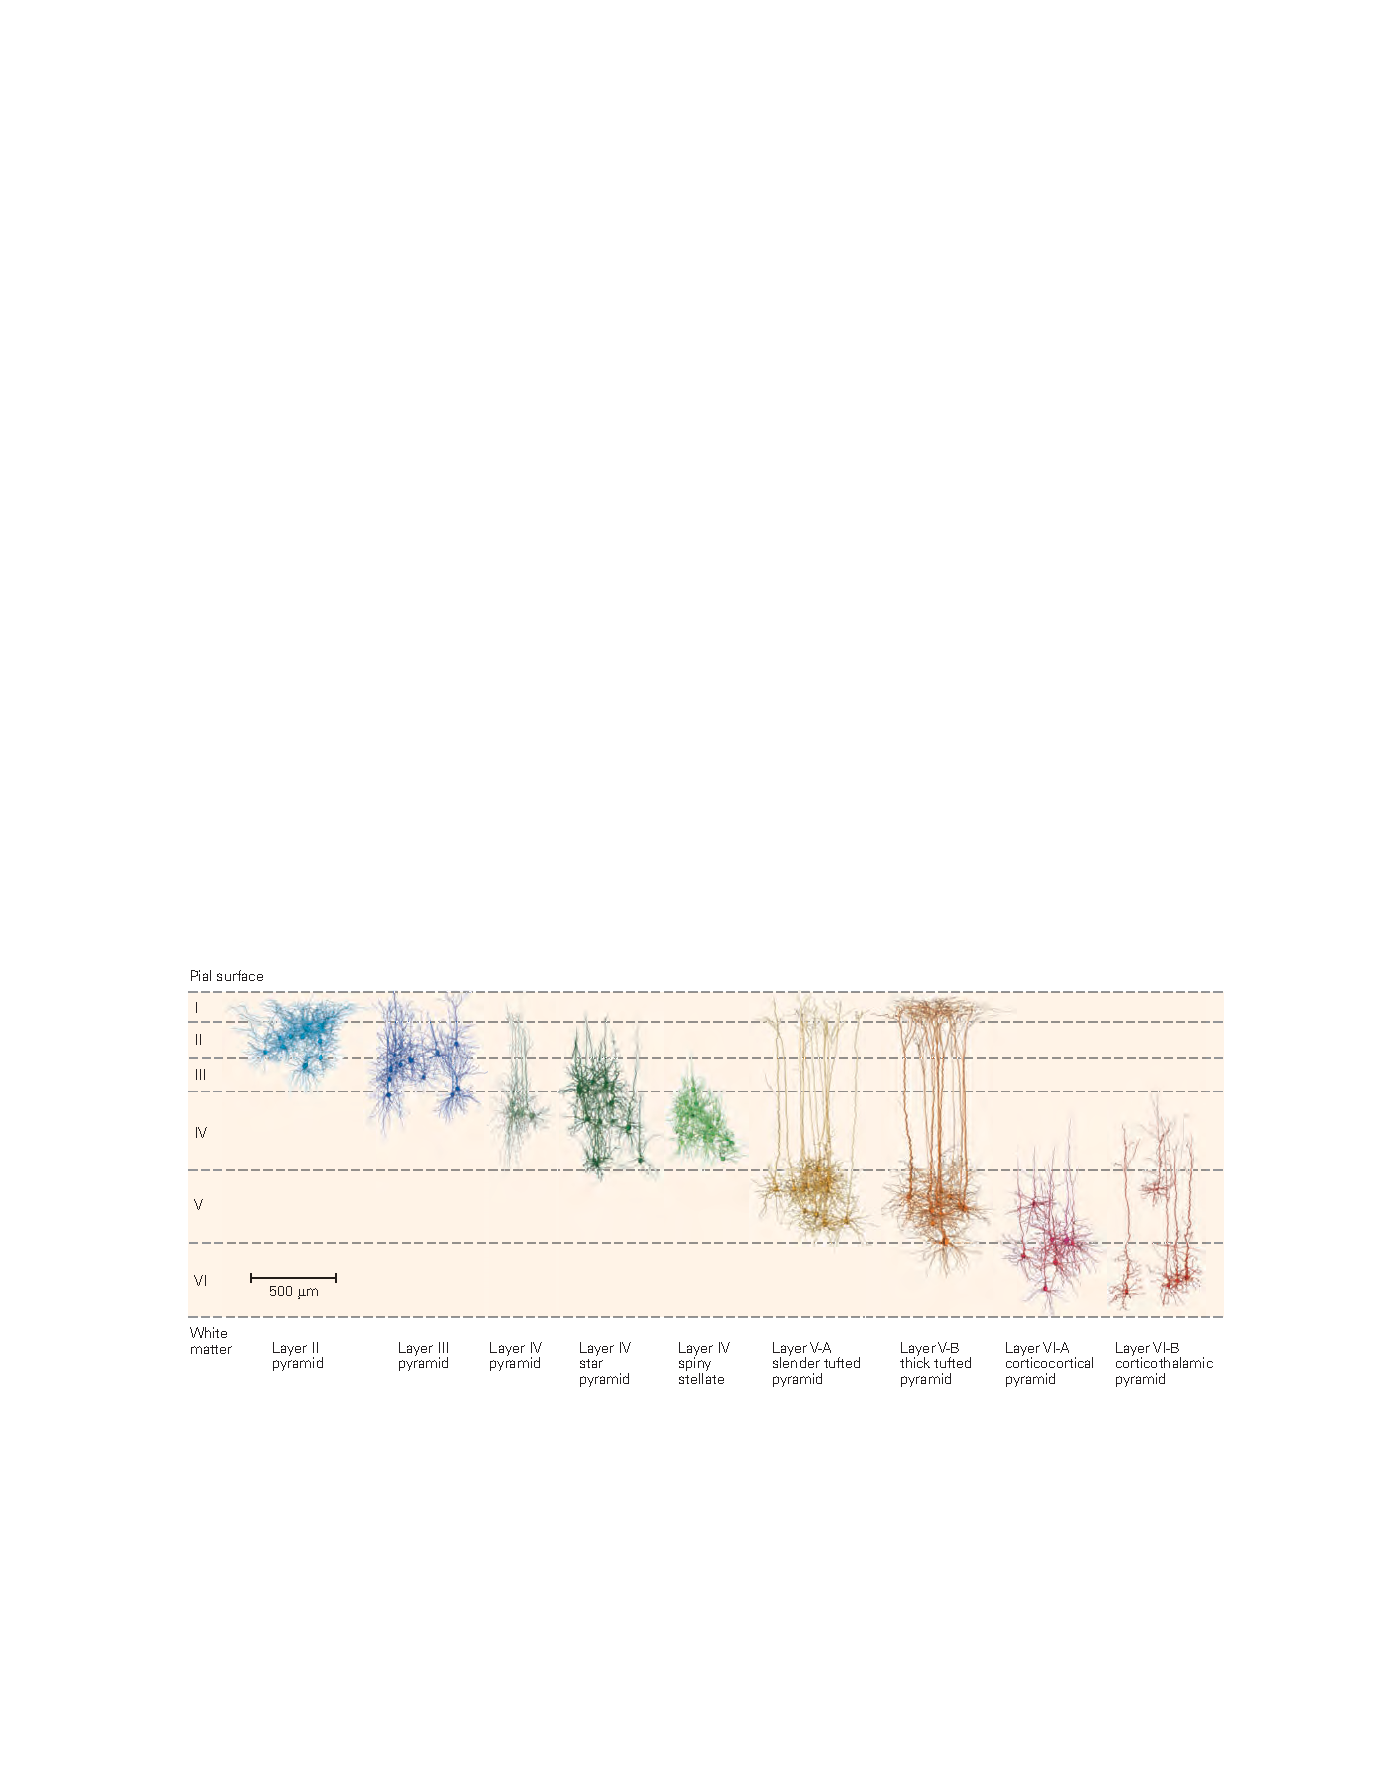
\includegraphics[width=1.0\linewidth]{chap19/fig_19_14}
	\caption{体感皮层的柱状组织。
		六层中的皮层兴奋性神经元具有独特的金字塔型形状,具有大细胞体、一个垂直向皮层表面突出并在更表层分枝的单个顶端树突,以及靠近细胞体分枝的多个基底树突。
		锥体神经元在大小、基因表达模式、顶端树突的长度和厚度以及轴突的投射目标方面存在差异。
		所有这些神经元都在大脑皮层内的目标上形成突触。
		此外,V 层的锥体神经元皮层下投射到脊髓、脑干、中脑和基底神经节。
		第六层的皮层丘脑神经元投射回传入丘脑核,为该柱提供感觉输入。
		第四层的多刺星状神经元是唯一显示的不是锥体神经元的兴奋性细胞\cite{oberlaender2012cell}。}
	\label{fig:19_14}
\end{figure}


锥体神经元构成躯体感觉皮层的主要兴奋类;
它们构成了大约 80\% 的\textit{初级躯体感觉皮层}神经元。 
六个皮层中每一层的锥体神经元投射到特定目标(图~\ref{fig:19_14})。
循环水平连接连接相同或相邻列中的锥体神经元,允许它们在被相同刺激同时激活时共享信息。
II 层和 III 层中的神经元也投射到同一列中的 V 层,投射到同一半球的更高皮层区域,并投射到相反半球的镜像位置。
这些与更高皮层区域的前馈连接允许复杂的信号整合,如本章后面所述。


V 层中的锥体神经元提供每一列的主要输出。
它们接收来自同一列和相邻列中 II 层和 III 层神经元的兴奋性输入以及稀疏的丘脑皮层输入。
V 层(V-A 层)表层部分的神经元将前馈输出双向发送到高阶皮层区域的 IV 层(参见图~\ref{fig:19_17}C)以及纹状体。
V 层(V-B 层)更深的神经元投射到皮层下结构,包括基底神经节、上丘、桥脑和其他脑干核团、脊髓和背柱核团。
第六层神经元投射到局部皮层神经元,然后返回丘脑,特别是投射到为该柱提供输入的腹侧后核区域。


\begin{figure}[htbp]
	\centering
	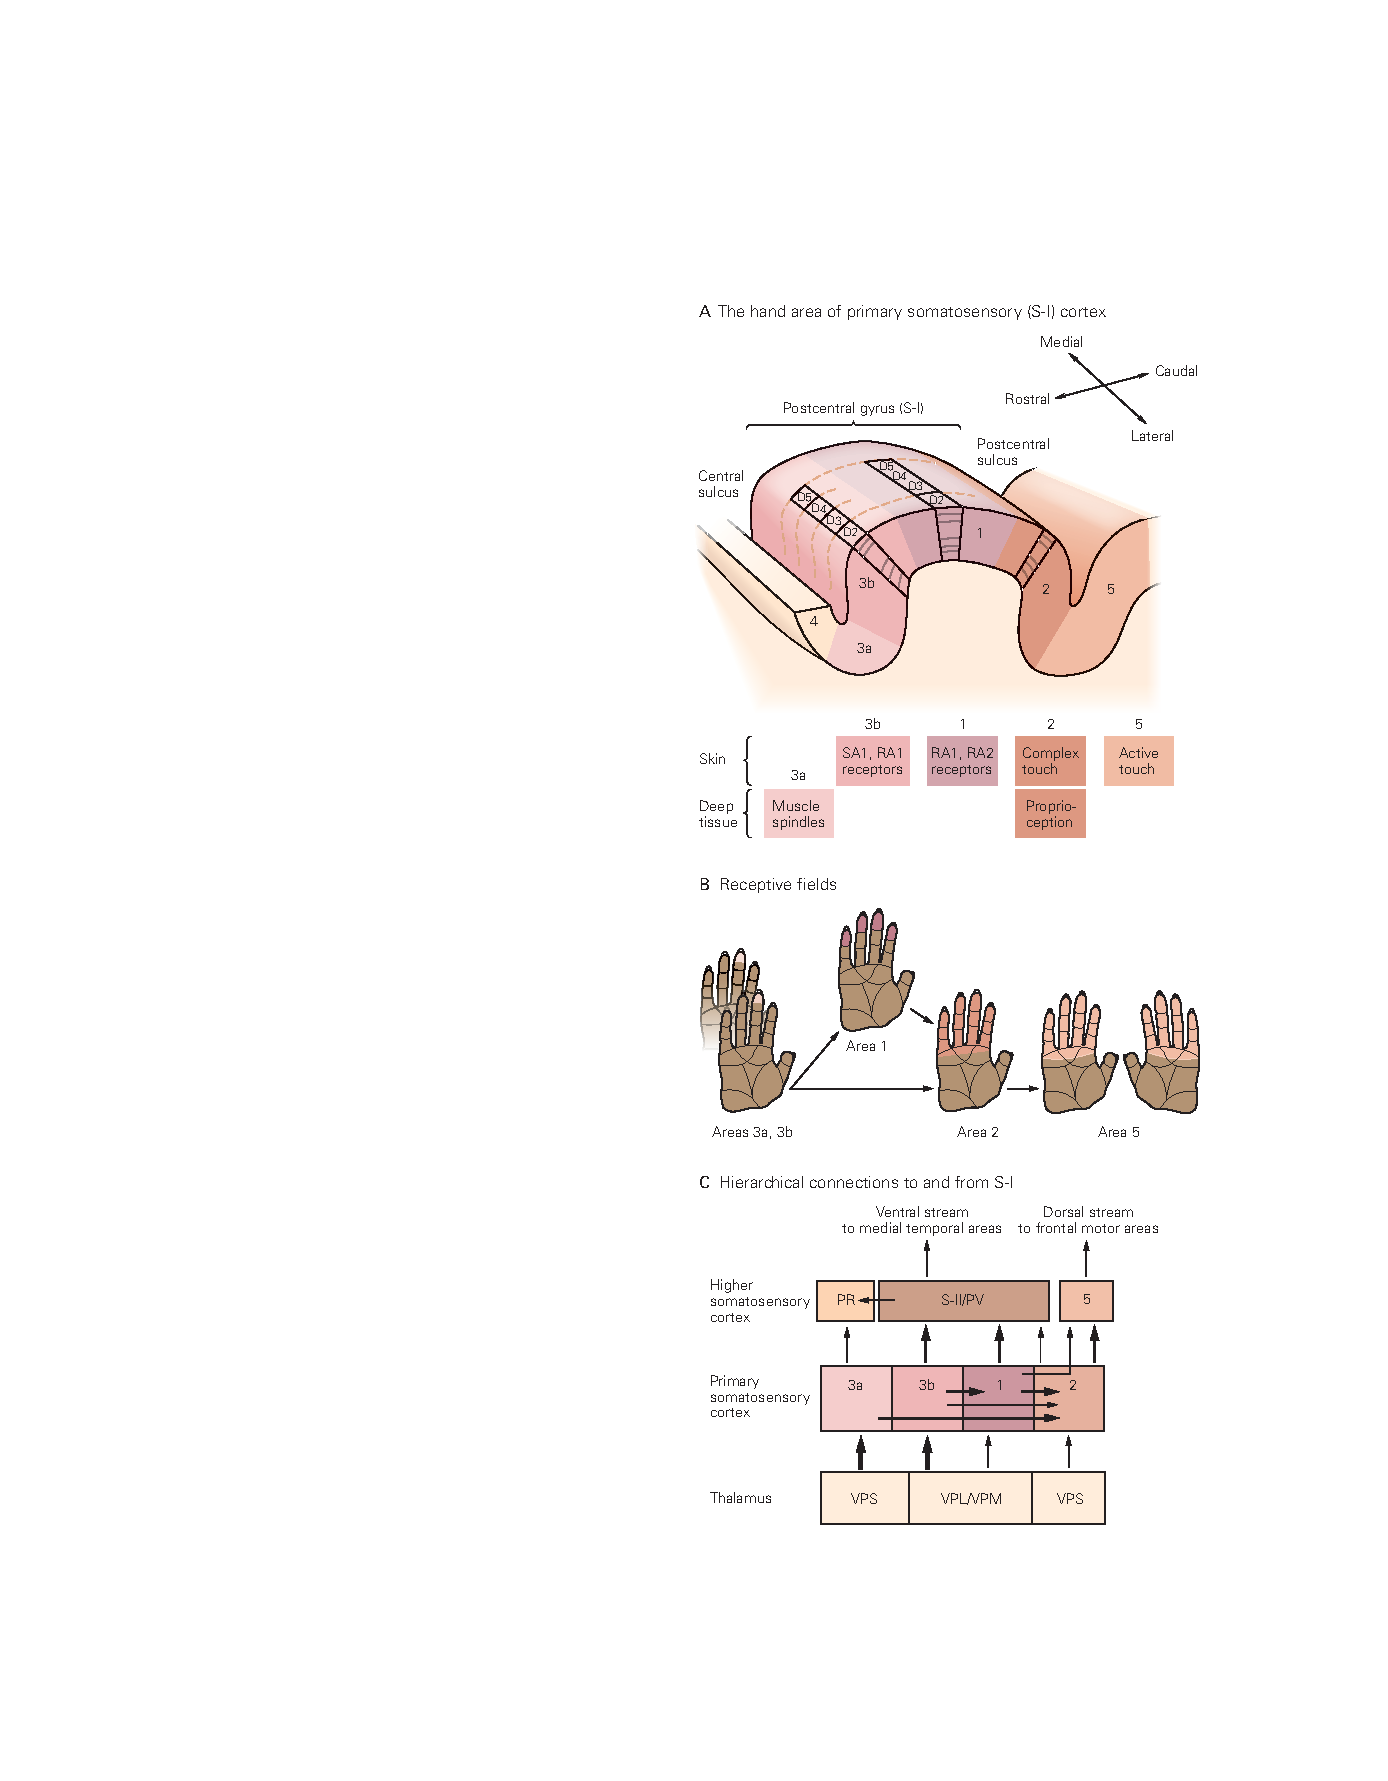
\includegraphics[width=0.5\linewidth]{chap19/fig_19_17}
	\caption{\textit{初级躯体感觉皮层}的手部区域。 
		\textbf{A.} 这个通过手部表示的矢状切面说明了人脑中\textit{初级躯体感觉皮层}的四个子区域(区域 3a、3b、1 和 2)以及相邻的初级运动皮层(区域 4)和后顶叶皮层(区域 5)。
		皮层表面上的标签表示代表各个手指的列(D2–D5);
		向右的箭头表示大脑中的部分方向。
		四个\textit{初级躯体感觉皮层}区域处理不同类型的体感信息,由皮层部分下方颜色匹配的矩形指示。
		区域 5 中的神经元主要响应以目标为导向的主动手部运动。
		\textbf{B.} 猕猴\textit{初级躯体感觉皮层}各区域神经元的典型感受野在手部图标上显示为彩色斑块。
		通过轻触皮肤或移动各个关节来勾勒出区域。
		感受野在区域 3a 和 3b 中最小,触觉信息首先进入大脑皮层,区域 1、2 和 5 中的感受野逐渐变大,反映出来自区域 3b 中的神经元的会聚输入,这些神经元在使用手时会一起受到刺激。
		区域 5 和\textit{次级躯体感觉皮层}皮层中的神经元通常具有双侧感受野,因为它们对双手镜像位置的触摸做出反应\cite{gardner1988somatosensory,iwamura1993rostrocaudal,iwamura1994bilateral}。
		\textbf{C.} 体感皮层区域之间的前馈层次连接。
		丘脑皮层和皮层皮层连接的强度由连接这些区域的箭头粗细表示。
		丘脑中的神经元主要将其轴突发送到区域 3a 和 3b,但有些也投射到区域 1 和 2。反过来,皮层区域 3a 和 3b 中的神经元投射到区域 1 和 2。
		来自\textit{初级躯体感觉皮层}四个区域的信息被传递 到后顶叶皮层(区域 5)和\textit{次级躯体感觉皮层}中的神经元。
		其中许多连接是双向的。
		高阶皮层区域的神经元投射回低阶区域,特别是 I 层。\cite{felleman1991distributed}。}
	\label{fig:19_17}
\end{figure}


除了来自触觉感受器的信息前馈信号外,来自较高体感皮层区域的第 II 层和第 III 层的反馈信号被提供给较低皮层区域的第 I 层,从而调节它们的兴奋性。
这种反馈信号不仅起源于躯体感觉皮层区域,还起源于后顶叶皮层的感觉运动区域、额叶运动区域、边缘区域以及参与记忆形成和存储的内侧颞叶区域。
这些反馈信号被认为在选择用于认知处理(通过注意力机制)和短期记忆任务的感觉信息方面发挥作用。
反馈通路也可能在运动活动期间控制感觉信号。
每列内的各种局部抑制性中间神经元用于聚焦柱状输出。



\subsection{皮层柱是按体位组织的}

初级躯体感觉皮层内的列按地形排列,因此在\textit{初级躯体感觉皮层}的四个区域中的每一个区域都有一个完整的躯体表示(图~\ref{fig:19_15})。
身体的皮层图大致对应于脊柱皮区(见图~\ref{fig:18_13})。
骶骨节段在内侧,腰椎和胸椎节段在中央,颈椎节段在外侧,面部的三叉神经节段在\textit{初级躯体感觉皮层}皮层的最外侧部分。
了解大脑中身体的神经图对于定位中风或头部外伤对皮层的损伤非常重要。


\begin{figure}[htbp]
	\centering
	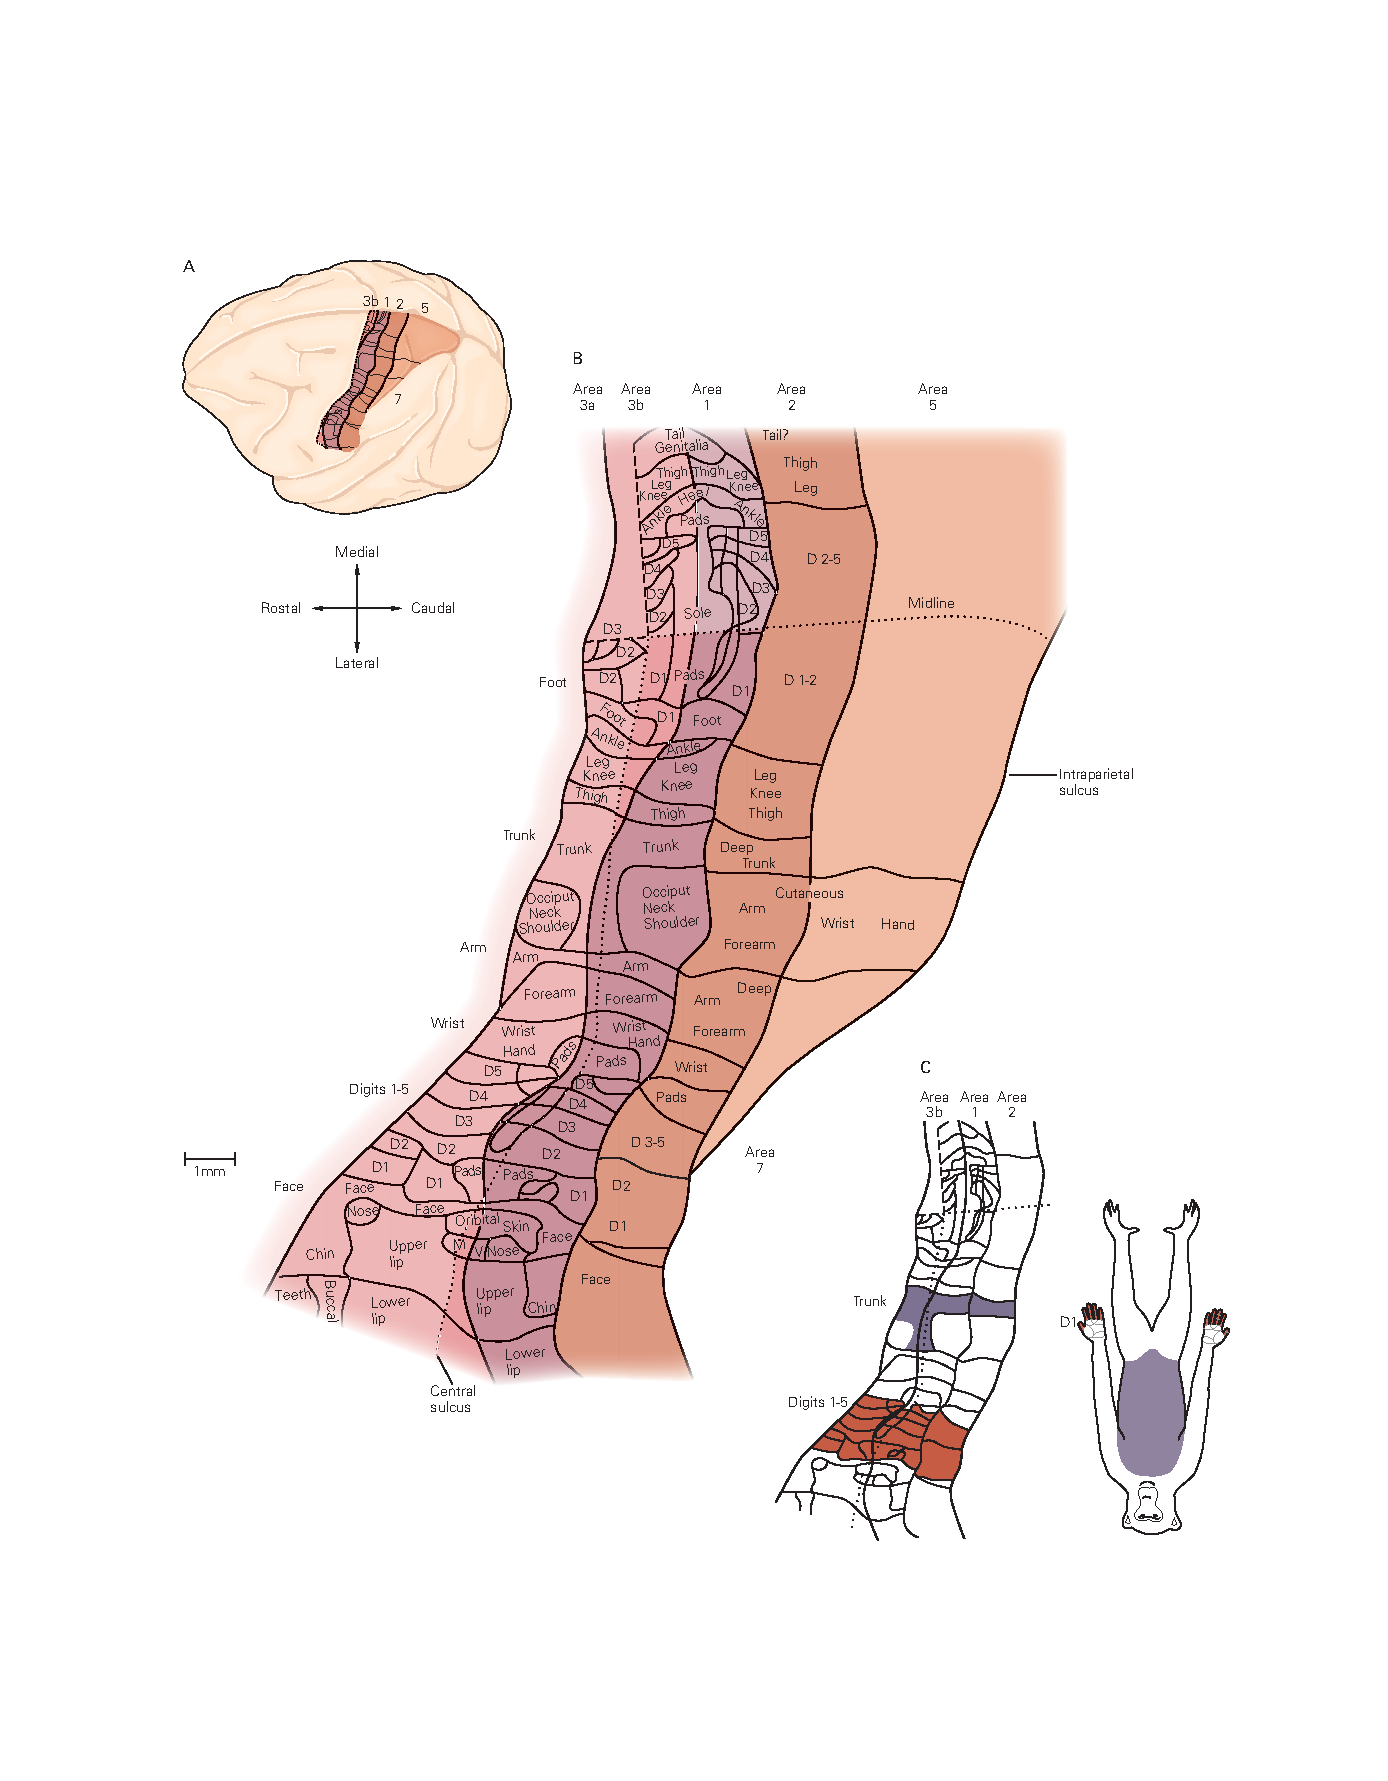
\includegraphics[width=0.95\linewidth]{chap19/fig_19_15}
	\caption{初级体感皮层的每个区域都包含整个身体表面的地形神经图\cite{nelson1980representations}。
		\textbf{A.} 与人脑一样,猕猴的初级体感皮层位于中央沟的尾部。
		猕猴皮层上的彩色区域对应于图~\ref{fig:19_12}~中人脑的同源布罗德曼区域。
		猕猴的第 5 区与人类的第 5 区和第 7 区同源。
		猕猴的第 7 区与人类的第 39 区和 40 区同源。
		\textbf{B.} 右边的平面图显示了猕猴的体感皮层沿着中央沟展开(与区域3b和1之间的边界平行的虚线)。
		该图的上部包括从半球内侧壁展开的皮层。
		身体图是从中央后回的微电极记录中获得的。
		身体表面被映射到按脊柱皮节顺序排列的头尾带内的列。
		区域 3b 和 1 中的身体图形成每个皮刀的远端-近端或背-腹轴的镜像。
		每个手指(D5–D1)在区域 3b 和区域 1 中沿皮层的内侧-外侧轴都有自己的表示,但来自几个相邻手指的输入会聚在区域 2 和区域 5 的神经元的感受野中。
		\textbf{C.} 皮层放大 高度神经支配的皮肤区域。
		尽管躯干(紫色)比手指(红色)覆盖的皮肤面积更大,但由于手指的神经支配密度更高,因此响应手指触摸的皮层柱数量几乎是触摸躯干时激活的数量的三倍 手指。}
	\label{fig:19_15}
\end{figure}


体表在顶叶中至少有 10 个不同的神经映射:
四个在\textit{初级躯体感觉皮层}中,四个在\textit{次级躯体感觉皮层}中,至少两个在后顶叶皮层中。
因此,这些区域调节触觉的不同方面。
\textit{初级躯体感觉皮层} 3b 和 1 区域中的神经元处理表面纹理的细节,而区域 2 中的神经元代表物体的大小和形状。
躯体感觉的这些属性在\textit{次级躯体感觉皮层}和后顶叶皮层中得到进一步阐述,神经元分别参与物体辨别和操纵。


体位图的另一个重要特征是分配给每个身体部位的大脑皮层数量。
人脑中身体的神经图,称为矮人,并不完全复制皮肤的空间地形。
相反,身体的每个部分都按照其对触觉的重要性来表示。 
不成比例的大面积用于某些身体区域,特别是手、足和嘴,而相对较小的区域用于更近端的身体部位。
在人类和猴子中,更多的皮层柱用于手指而不是整个躯干(图~\ref{fig:19_15} C)。


用于单位面积皮肤的皮层面积的数量(称为皮层放大率)在不同的身体表面上相差超过一百倍。
它与神经支配密度密切相关,因此与皮肤区域中触觉感受器的空间敏锐度密切相关。
人类大脑中放大倍数最大的区域(嘴唇、舌头、手指和脚趾)的触觉敏锐度阈值分别为 0.5、0.6、1.0 和 4.5 毫米。


啮齿动物和其他用胡须探测环境的哺乳动物在\textit{初级躯体感觉皮层}中有大量列,称为桶,接收来自面部单个触须的输入(方框~\ref{box:19_2})。
桶状皮层为研究皮层回路提供了广泛使用的实验准备。



\begin{proposition}[啮齿动物须桶系统] \label{box:19_2}
	
	\quad \quad 啮齿类动物须筒系统是现代神经科学中广泛使用的动物模型。
	,大多数哺乳动物和所有灵长类动物的脸上都有特殊的触觉毛发,称为触须。
	与皮肤上的其他毛发不同,触须生长于毛囊中,毛囊由三叉神经支配,周围是充满血液的窦。
	
\end{proposition}


\begin{figure}[htbp]
	\centering
	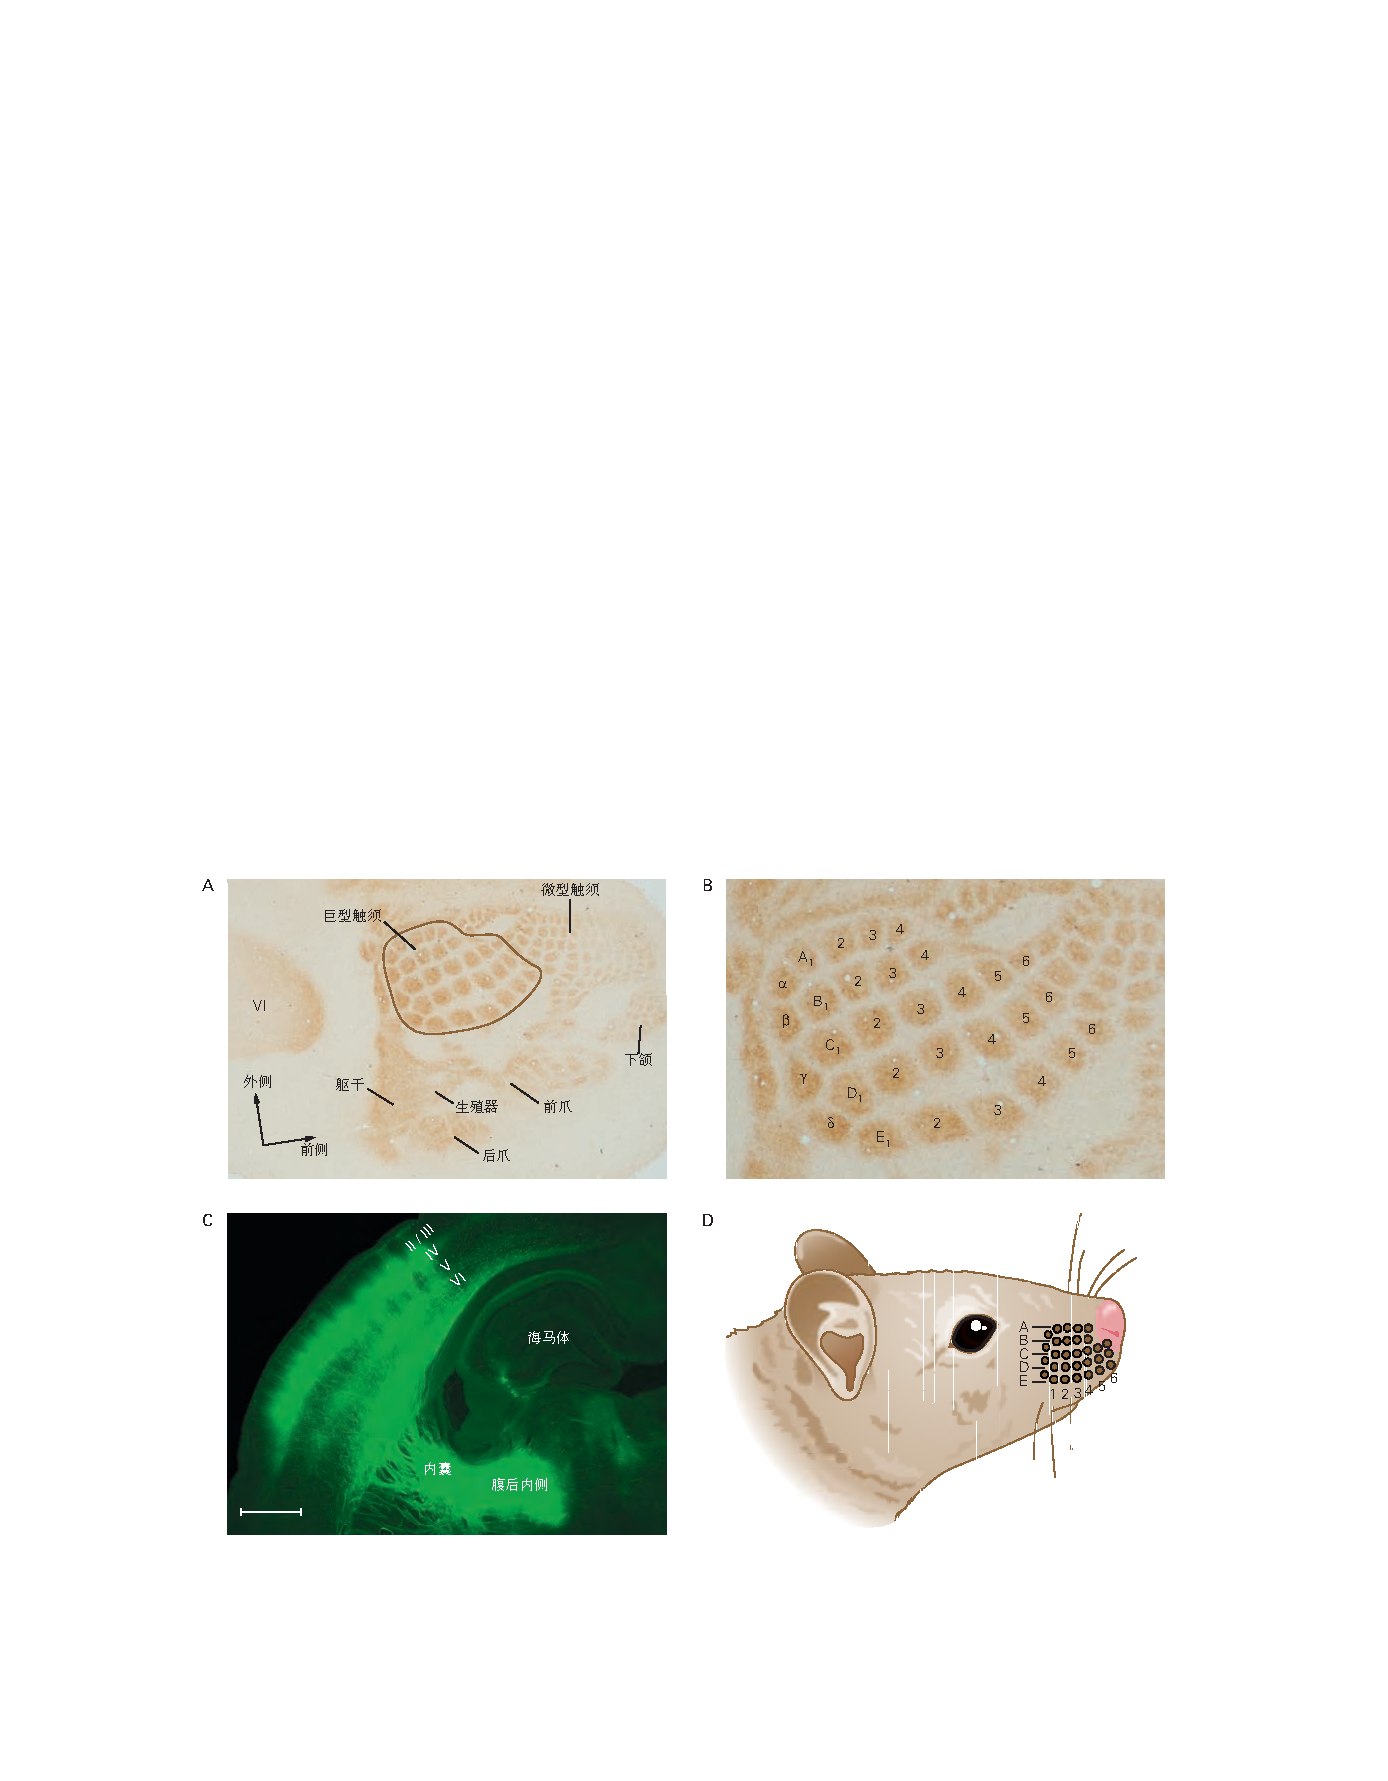
\includegraphics[width=1.0\linewidth]{chap19/fig_19_16}
	\caption{啮齿类动物的“桶状皮层”代表了地形图案中的振颤。
		筒状皮层是啮齿类动物\textit{初级躯体感觉皮层}的一个亚区域,代表面部触须,是一种被广泛研究的用于破译皮层回路的结构。
		\textbf{A.} 经血清素染色的幼年大鼠体感皮层第四层切向组织学切片。
		较暗的免疫反应斑块对应于特定身体部位的皮层表现。
		啮齿类动物体感皮层图的最大部分专门用于触须。
		\textbf{B.} \textit{初级躯体感觉皮层}中宏观振动表现的放大视图。
		脸上胡须的空间模式是根据动物而定的,允许每个皮层“桶”通过带有字母的行和带有相应胡须数量的弧(列)来识别。
		每个桶中的神经元对这根主要胡须的运动反应最为强烈。
		\textbf{C.} 沿着轴突从丘脑\textit{腹后内侧}核到\textit{初级躯体感觉皮层}的路径倾斜切割的大鼠脑切片。
		绿色荧光蛋白标记的\textit{腹后内侧}轴突通过\textit{内囊}投射到皮层下白质,并在进入皮层之前平行于软脑膜表面行进。
		轴突密集地支配第四层,在那里它们形成离散的管状体,并更稀疏和扩散地支配第五层和第六层的边界。
		比例尺=1 毫米。
		\textbf{D.} 皮层中管状体的地形排列与面部振动的空间排列成行(字母)和弧(数字)相匹配。}
	\label{fig:19_16}
\end{figure}



\subsection{皮层神经元的感受野整合来自邻近受体的信息}

\textit{初级躯体感觉皮层}中的神经元至少是皮肤中触觉感受器之外的三个突触。
他们的输入代表在背柱核、丘脑和皮层本身处理的信息。 
每个皮层神经元接收来自皮肤特定区域的受体的输入,这些输入一起构成它的感受野。
我们认为皮肤上的特定位置被触摸是因为皮层中特定的神经元群被激活。
这种体验可以通过对相同皮层神经元的电刺激或光遗传学刺激进行实验诱导。


皮层神经元的感受野比周围神经中的体感纤维大得多。
例如,支配指尖的\textit{慢适应1型}和\textit{快适应1型}纤维的感受野是皮肤上的小点(图~\ref{fig:19_5}),而接收这些输入的皮层神经元的感受野覆盖整个指尖或几个相邻的手指(图~\ref{fig:19_17}B)。
区域 3b 中神经元的感受野代表 300 到 400 根神经纤维的输入复合,通常覆盖单个指骨或掌垫。
来自同一皮肤区域的\textit{慢适应1型}和\textit{快适应1型}触觉感受器的输入会聚到区域 3b 中的共同神经元。


较高皮层区域的感受野甚至更大,跨越在运动活动期间同时激活的皮肤功能区域。
这些包括几个相邻手指的指尖,或整个手指,或手指和手掌。
\textit{初级躯体感觉皮层} 1 和 2 区域中的神经元关注的信息比它们在身体上的神经支配部位更抽象。
当同时触摸多个手指时,其感受野包括一根以上手指的神经元会以更高的速率放电,并以这种方式发出手中物体的大小和形状的信号。
这些大的感受野允许皮层神经元整合来自各个触觉感受器的碎片化信息,使我们能够识别物体的整体形状。
例如,这样的神经元可以区分螺丝刀的手柄和刀刃。


来自\textit{初级躯体感觉皮层}中不同感觉受体的会聚输入也可能允许单个神经元检测物体的大小和形状。
区域 3b 和 1 中的神经元仅对触摸有反应,而区域 3a 中的神经元对肌肉拉伸有反应,而区域 2 中的许多神经元都接收这两种输入。
因此,区域 2 中的神经元可以整合有关用于抓取物体的手形、手施加的握力以及物体产生的触觉刺激的信息;
这种综合信息可能足以识别物体。


皮层神经元的感受野通常有一个被抑制区包围或叠加的兴奋区(图~\ref{fig:19_18} 觉刺激的反应。
类似地,感受野内的重复刺激也可能降低神经元反应性,因为该通路的兴奋性因局部中间神经元介导的更持久抑制而减弱。


\begin{figure}[htbp]
	\centering
	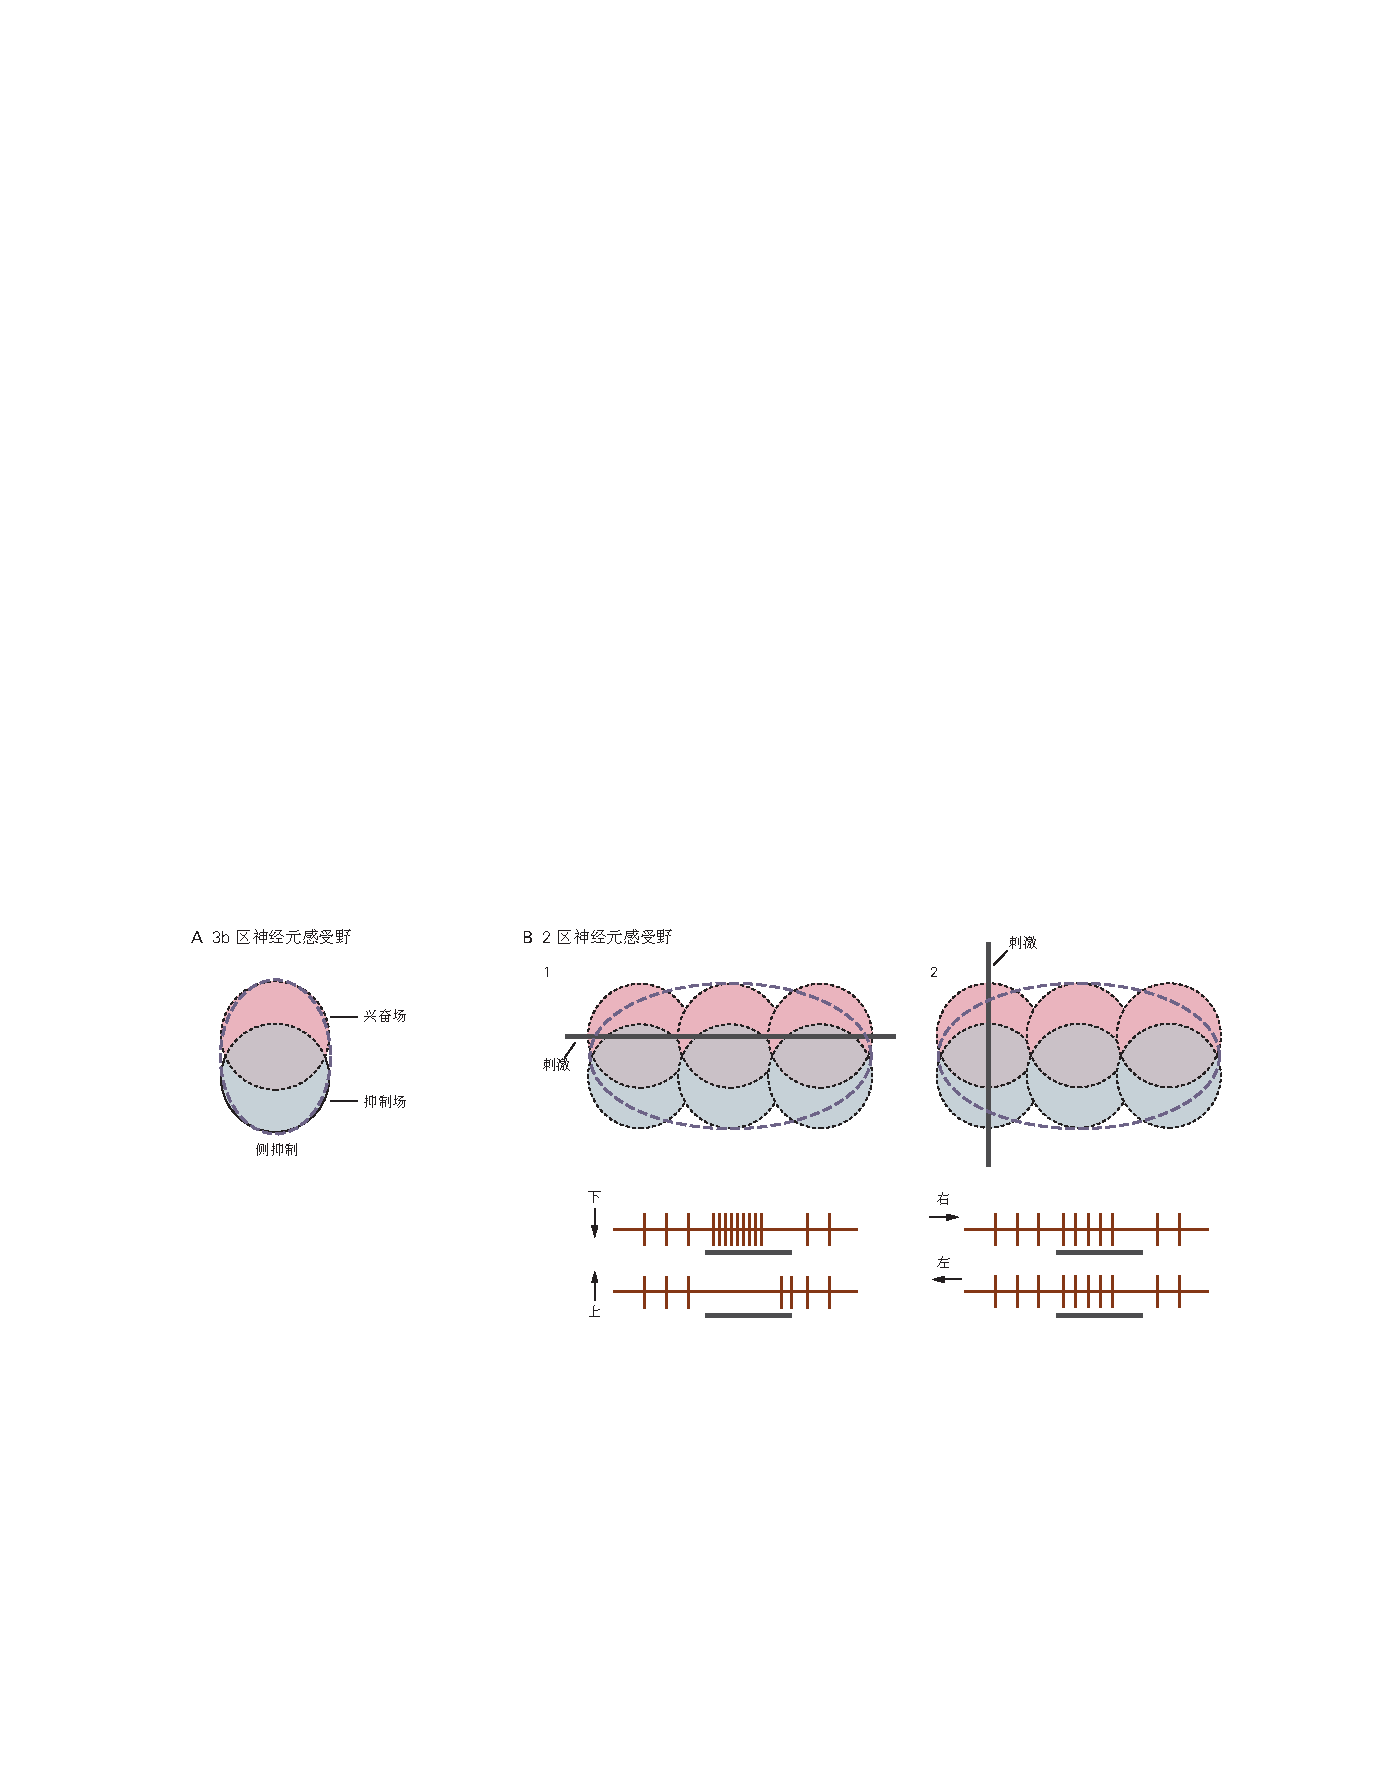
\includegraphics[width=1.0\linewidth]{chap19/fig_19_18}
	\caption{皮层神经元的兴奋性和抑制性输入的空间排列决定了哪些刺激特征由神经元编码。
		\textbf{A.} 初级躯体感觉皮层 3b 区的神经元在其感受野内具有重叠的兴奋区和抑制区\cite{dicarlo1998structure,sripati2006spatiotemporal}。
		\textbf{B.} 具有相同兴奋区和抑制区排列的三个突触前神经元的聚合允许神经元中的方向和定向选择性 在区域 2。 
		1. 水平杆向下运动穿过突触后细胞的感受野会产生强烈的兴奋反应,因为同时接触所有三个突触前神经元的兴奋场。
		酒吧的向上运动强烈抑制射击,因为它首先进入所有三个抑制区域。
		神经元对通过兴奋场的向上运动反应不佳,因为最初的抑制比刺激持续更久。
		2. 垂直条穿过感受野的运动会引起微弱的反应,因为它同时穿过输入神经元的兴奋性和抑制性感受野。
		在此示例中无法区分向左或向右的运动。}
	\label{fig:19_18}
\end{figure}


抑制性感受野是通过背柱核、丘脑和皮层本身中的中间神经元的前馈和反馈连接产生的,它们限制了兴奋的传播。 
由一个回路中的强烈活动产生的抑制作用会降低附近仅处于微弱兴奋状态的神经元的输出。
抑制网络确保传递几种竞争反应中最强的一种,从而允许采用赢者通吃的策略。
当大量的触摸神经元受到刺激时,这些回路可以防止纹理等触觉细节模糊。
此外,当手用于熟练任务时,大脑中的高层中枢会使用抑制回路,通过抑制不需要的、分散注意力的输入,将注意力集中在手的相关信息上。


感受野在皮肤上的大小和位置不是永久固定的,而是可以根据经验或感觉神经的损伤进行修改(第~\ref{chap:chap53}~章)。
皮层感受野似乎是在发育过程中形成的,并通过同时激活输入通路来维持。
如果周围神经受伤或被横切,其皮层投射目标会从通常被抑制网络抑制的不太有效的感觉输入,或从保留神经支配的邻近皮肤区域新开发的连接中获得新的感受野。
同样,通过重复练习广泛刺激传入通路可能会加强突触输入,从而改善知觉,从而提高表现。



\section{触摸信息在连续的中央突触中变得越来越抽象}

体感信息从\textit{初级躯体感觉皮层}的四个区域并行传递到皮层的更高中心,例如\textit{次级躯体感觉皮层}、后顶叶皮层和初级运动皮层(图~\ref{fig:19_17} C)。
随着信息流向更高阶的皮层区域,需要特定的刺激模式组合来激发单个神经元。


来自邻近神经元的信号在更高的皮层区域被组合以辨别物体的全局特性,例如它们在手上的方向或运动方向(图~\ref{fig:19_19})。
一般来说,较高皮层区域的皮层神经元关注独立于其感受野中刺激位置的感觉特征,抽象出特定类别刺激共有的对象属性。


\begin{figure}[htbp]
	\centering
	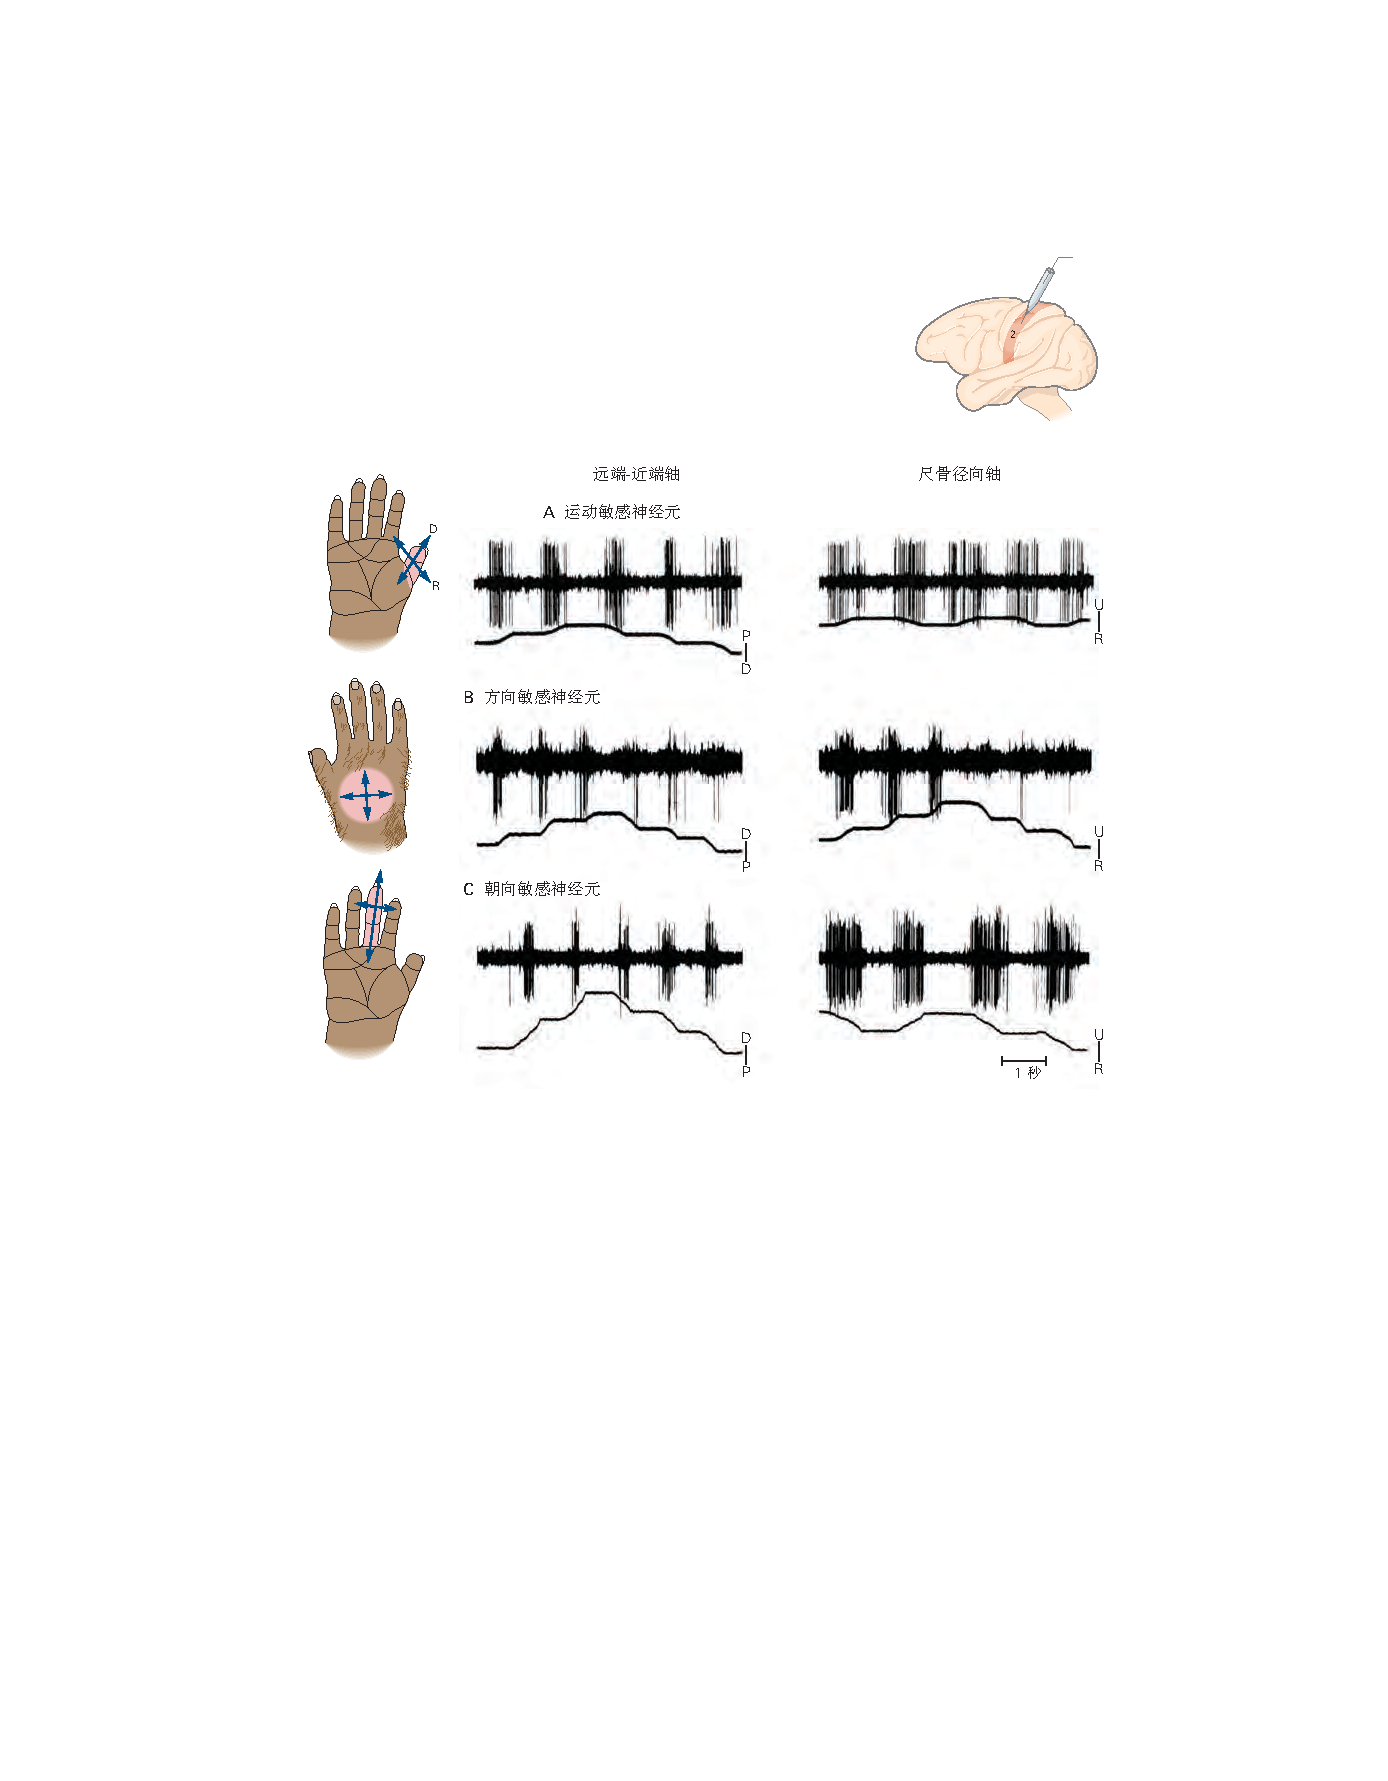
\includegraphics[width=1.0\linewidth]{chap19/fig_19_19}
	\caption{区域 2 中的神经元编码复杂的触觉信息。 
		这些神经元对探针穿过感受野的运动做出反应,但不会接触到单个点。
		下面的迹线表示向上和向下偏转的运动方向\cite{warren1986objective}。
		\textbf{A.} 运动敏感神经元对在各个方向抚摸皮肤做出反应。
		\textbf{B.} 方向敏感的神经元对朝向手掌尺侧的运动反应强烈,但对相反方向的运动没有反应。
		对远端或近端运动的反应较弱。
		\textbf{C.} 方向敏感的神经元对横跨手指(尺桡)的运动比对沿手指(远端-近端)的运动反应更好,但不区分尺骨与桡骨或近端与远端方向。}
	\label{fig:19_19}
\end{figure}


由于突触前感受野的空间排列,皮层神经元能够检测边缘的方向或运动方向。
兴奋性突触前神经元的感受野通常沿着一个公共轴对齐,该轴生成突触后神经元的首选方向。
此外,位于兴奋区一侧的抑制性突触前神经元的感受野增强了突触后神经元的定向和方向选择性(图~\ref{fig:19_18} B)。



\subsection{认知触觉由次级躯体感觉皮层中的神经元介导}

\textit{初级躯体感觉皮层}神经元对触摸的反应主要取决于神经元感受野内的输入。
这种前馈通路通常被描述为自下而上的过程,因为外围的受体是\textit{初级躯体感觉皮层}皮层神经元兴奋的主要来源。


高阶体感区域不仅从外周受体接收信息,而且还受到自上而下的认知过程的强烈影响,例如目标设定和注意力调节。
从各种研究中获得的数据(猴子的单神经元研究、人类神经影像学研究以及高阶体感区域受损患者的临床观察)表明顶叶的腹侧和背侧区域在触觉系统中起着互补的作用 类似于视觉系统的“什么”和“哪里”通路(见图~\ref{fig:17_13})。


\textit{次级躯体感觉皮层}位于人类和猴子外侧沟的上岸和相邻的顶叶盖(图~\ref{fig:19_12}B~和~\ref{fig:19_20}B)。
与\textit{初级躯体感觉皮层}一样,\textit{次级躯体感觉皮层}包含四个不同的解剖学子区域,具有单独的身体图。
中央区域(由\textit{次级躯体感觉皮层}本身和相邻的顶叶腹侧区域组成)接收来自区域 3b 和 1 的主要输入,主要是来自手和面部的触觉信息。
一个更靠近头端的区域,即顶叶腹侧区域,从区域 3a 接收有关主动手部运动的信息以及来自区域 3b 和 1 的触觉信息(图~\ref{fig:19_20})。
外侧沟最尾端的体感区域延伸到顶叶盖(图~\ref{fig:19_12}A)。
该区域紧靠后顶叶皮层,并在整合物体的体感和视觉特性方面发挥作用。


\begin{figure}[htbp]
	\centering
	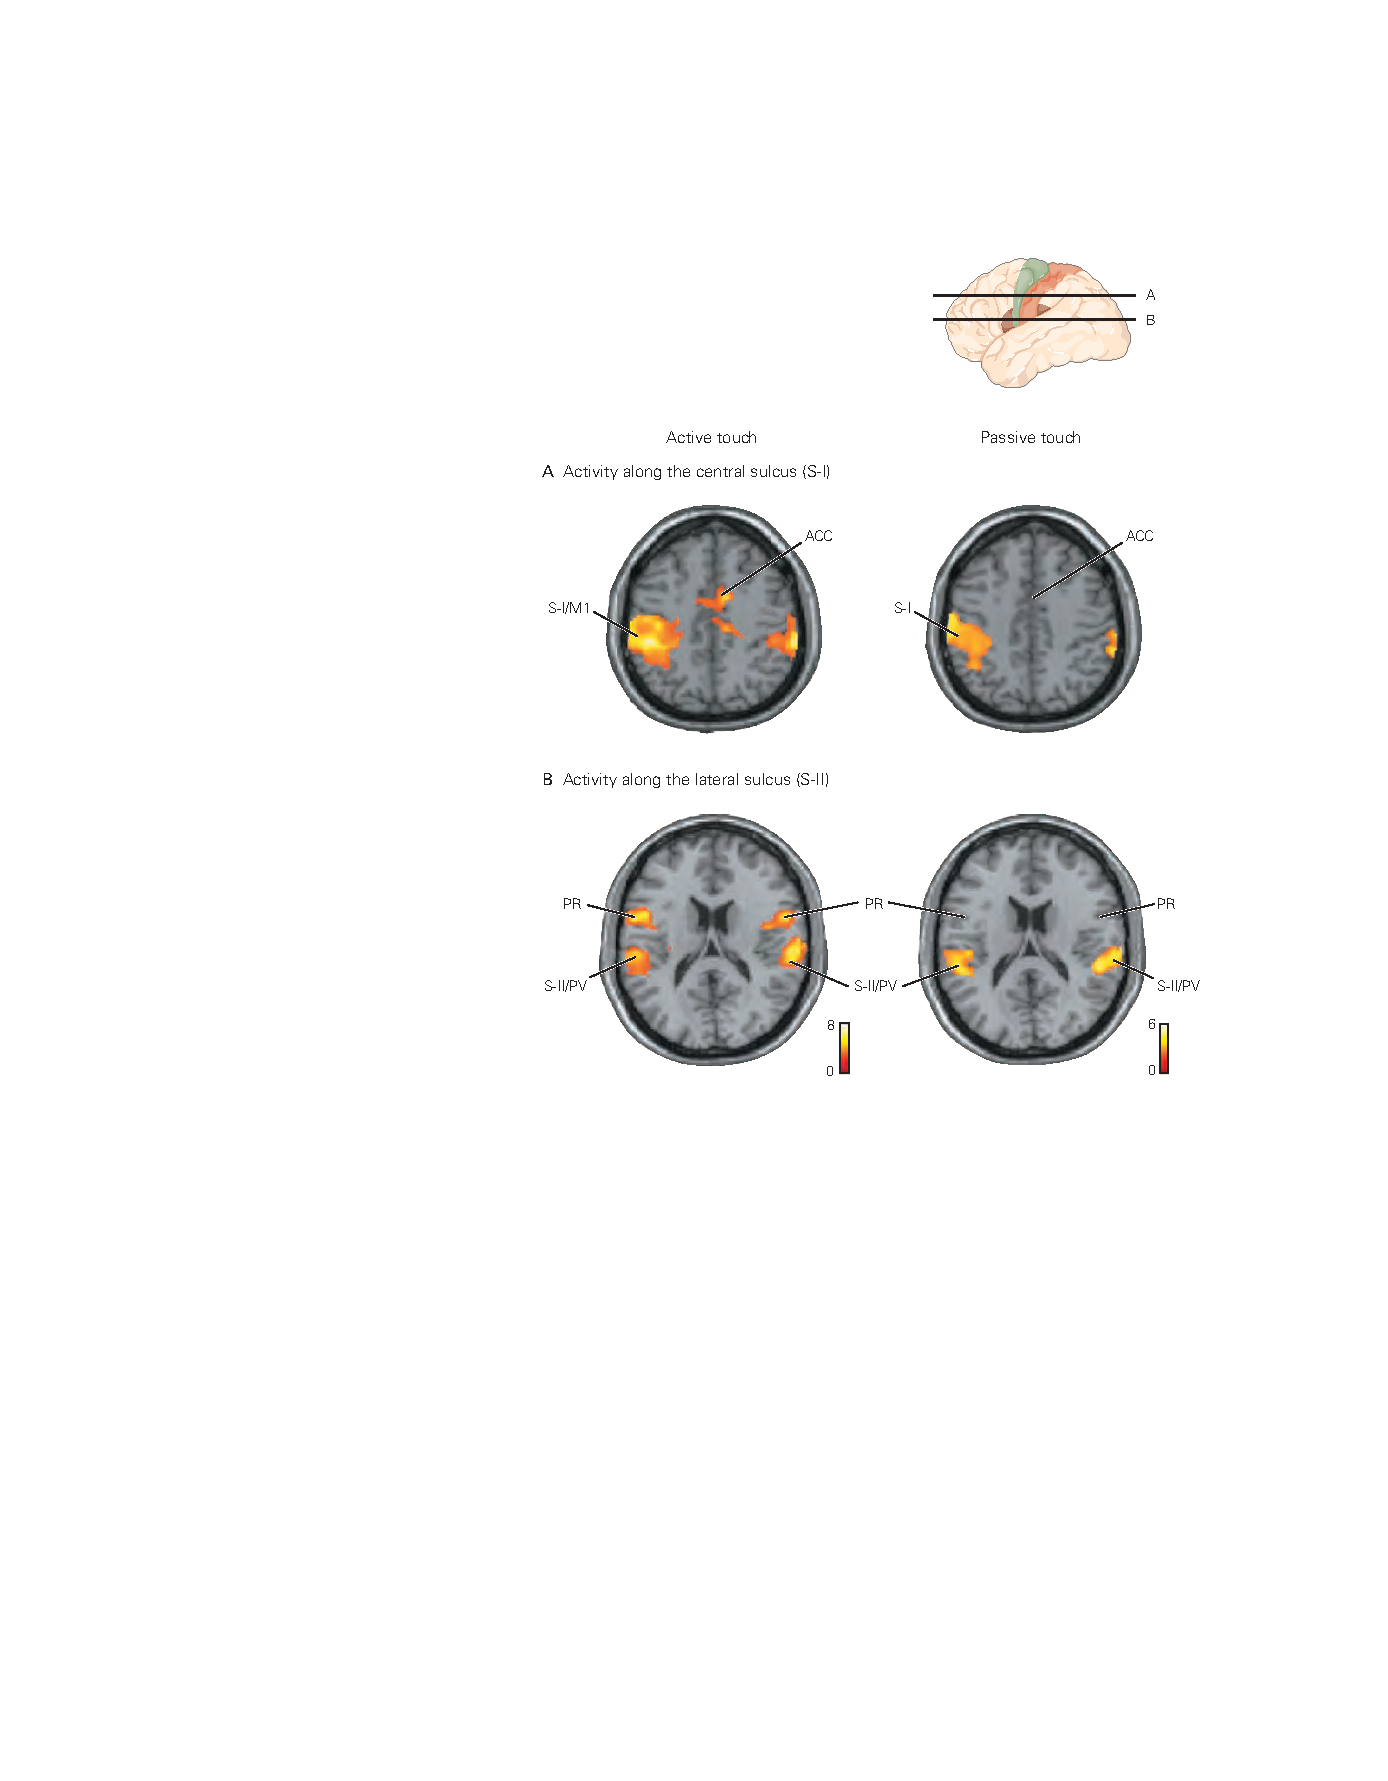
\includegraphics[width=0.85\linewidth]{chap19/fig_19_20}
	\caption{\textit{初级躯体感觉皮层}和\textit{次级躯体感觉皮层}中对主动触摸的反应比被动触摸引起的反应更复杂。
		使用\textit{功能性磁共振成像}对人脑中受被动和主动触摸刺激的皮层区域进行定位\cite{hinkley2007sensorimotor}。
		\textbf{A.} 右手用海绵被动抚摸(右图)和主动触摸海绵(左图)期间中央沟活动的轴向视图。 在这两种情况下,左半球的 3b 区和 1 区都被激活。
		主动触摸还涉及左半球的\textit{初级运动皮层}、\textit{前扣带皮层},并引起同侧\textit{初级躯体感觉皮层}(右半球)的微弱活动。
		这些位点在同一受试者中使用脑磁图独立确认。
		\textbf{B.} 同一实验中沿外侧裂活动的轴向视图。
		在被动抚摸期间,双侧活动发生在\textit{次级躯体感觉皮层}和\textit{顶叶腹侧皮层}区域,并且当受试者主动移动手时会更强。
		\textit{顶叶头腹侧皮层}仅在主动触摸期间处于活动状态。
		\textit{次级躯体感觉皮层}/\textit{顶叶腹侧皮层}和\textit{顶叶头腹侧皮层}中的脑磁图反应发生晚于\textit{初级躯体感觉皮层},反映了从\textit{初级躯体感觉皮层}到\textit{次级躯体感觉皮层}/\textit{顶叶腹侧皮层}以及从\textit{次级躯体感觉皮层}/\textit{顶叶腹侧皮层}到\textit{顶叶头腹侧皮层}的一系列触摸处理。}
	\label{fig:19_20}
\end{figure}


生理学研究表明,\textit{次级躯体感觉皮层}在手部物体的触觉识别(立体视觉)、区分空间特征(例如形状和纹理)以及时间特性(例如振动频率)方面起着关键作用。
\textit{次级躯体感觉皮层}神经元的感受野比\textit{初级躯体感觉皮层}大,覆盖手的整个表面,并且通常是双侧的,代表对侧和同侧手上对称的镜像位置。
如此大的感受野使我们能够感知一只手抓住的整个大物体的形状,使我们能够在工具接触手掌和不同手指时整合工具的整体轮廓。
双侧感受野使我们能够用两只手感知更大的物体,例如西瓜或篮球,在它们之间分担负荷。


\textit{次级躯体感觉皮层}神经元的大感受野也影响它们对运动和振动的生理反应。
\textit{次级躯体感觉皮层}神经元不将振动表示为与振荡频率相关的周期性尖峰序列,皮肤或\textit{初级躯体感觉皮层}神经元的感觉纤维也是如此(图~\ref{fig:19_9})。
相反,\textit{次级躯体感觉皮层}神经元抽象出振动刺激的时间或强度特性,以不同的平均速率针对不同的频率发射。
从时间编码神经元到速率编码神经元的类似频率依赖性转变是初级听觉皮层(第~\ref{chap:chap28}~章)中声音处理的基础,初级听觉皮层是与顶叶盖中的\textit{次级躯体感觉皮层}皮层并列的大脑区域。


重要的是,\textit{次级躯体感觉皮层}神经元的放电率取决于主体的行为背景或动机状态。
在最近的优雅研究中,\textit{拉努尔福$\cdot$罗莫}和他的同事比较了猴子在\textit{初级躯体感觉皮层}、\textit{次级躯体感觉皮层}和额叶不同区域对神经元振动刺激的反应,同时这些动物执行了两种选择的强制选择任务。
如果动物正确识别出两种振动刺激中哪一种频率更高,它们就会得到奖励。


\textit{初级躯体感觉皮层}中的神经元使用时间编码忠实地代表每个刺激的振动周期:它们与每个周期同相发射短暂的尖峰脉冲(图~\ref{fig:19_9}B)。
相反,\textit{次级躯体感觉皮层}神经元以非周期性尖峰序列响应第一个刺激,其中它们的平均放电率与振动频率直接或负相关(图~\ref{fig:19_21}A)。
他们对第二个刺激的反应更加抽象。
\textit{次级躯体感觉皮层}脉冲序列结合了两种刺激的频率(图~\ref{fig:19_21}B)。
换句话说,\textit{次级躯体感觉皮层}对振动的反应取决于刺激环境:
相同的振动刺激可以引起不同的放电率,这取决于前一个刺激的频率是更高还是更低。


\begin{figure}[htbp]
	\centering
	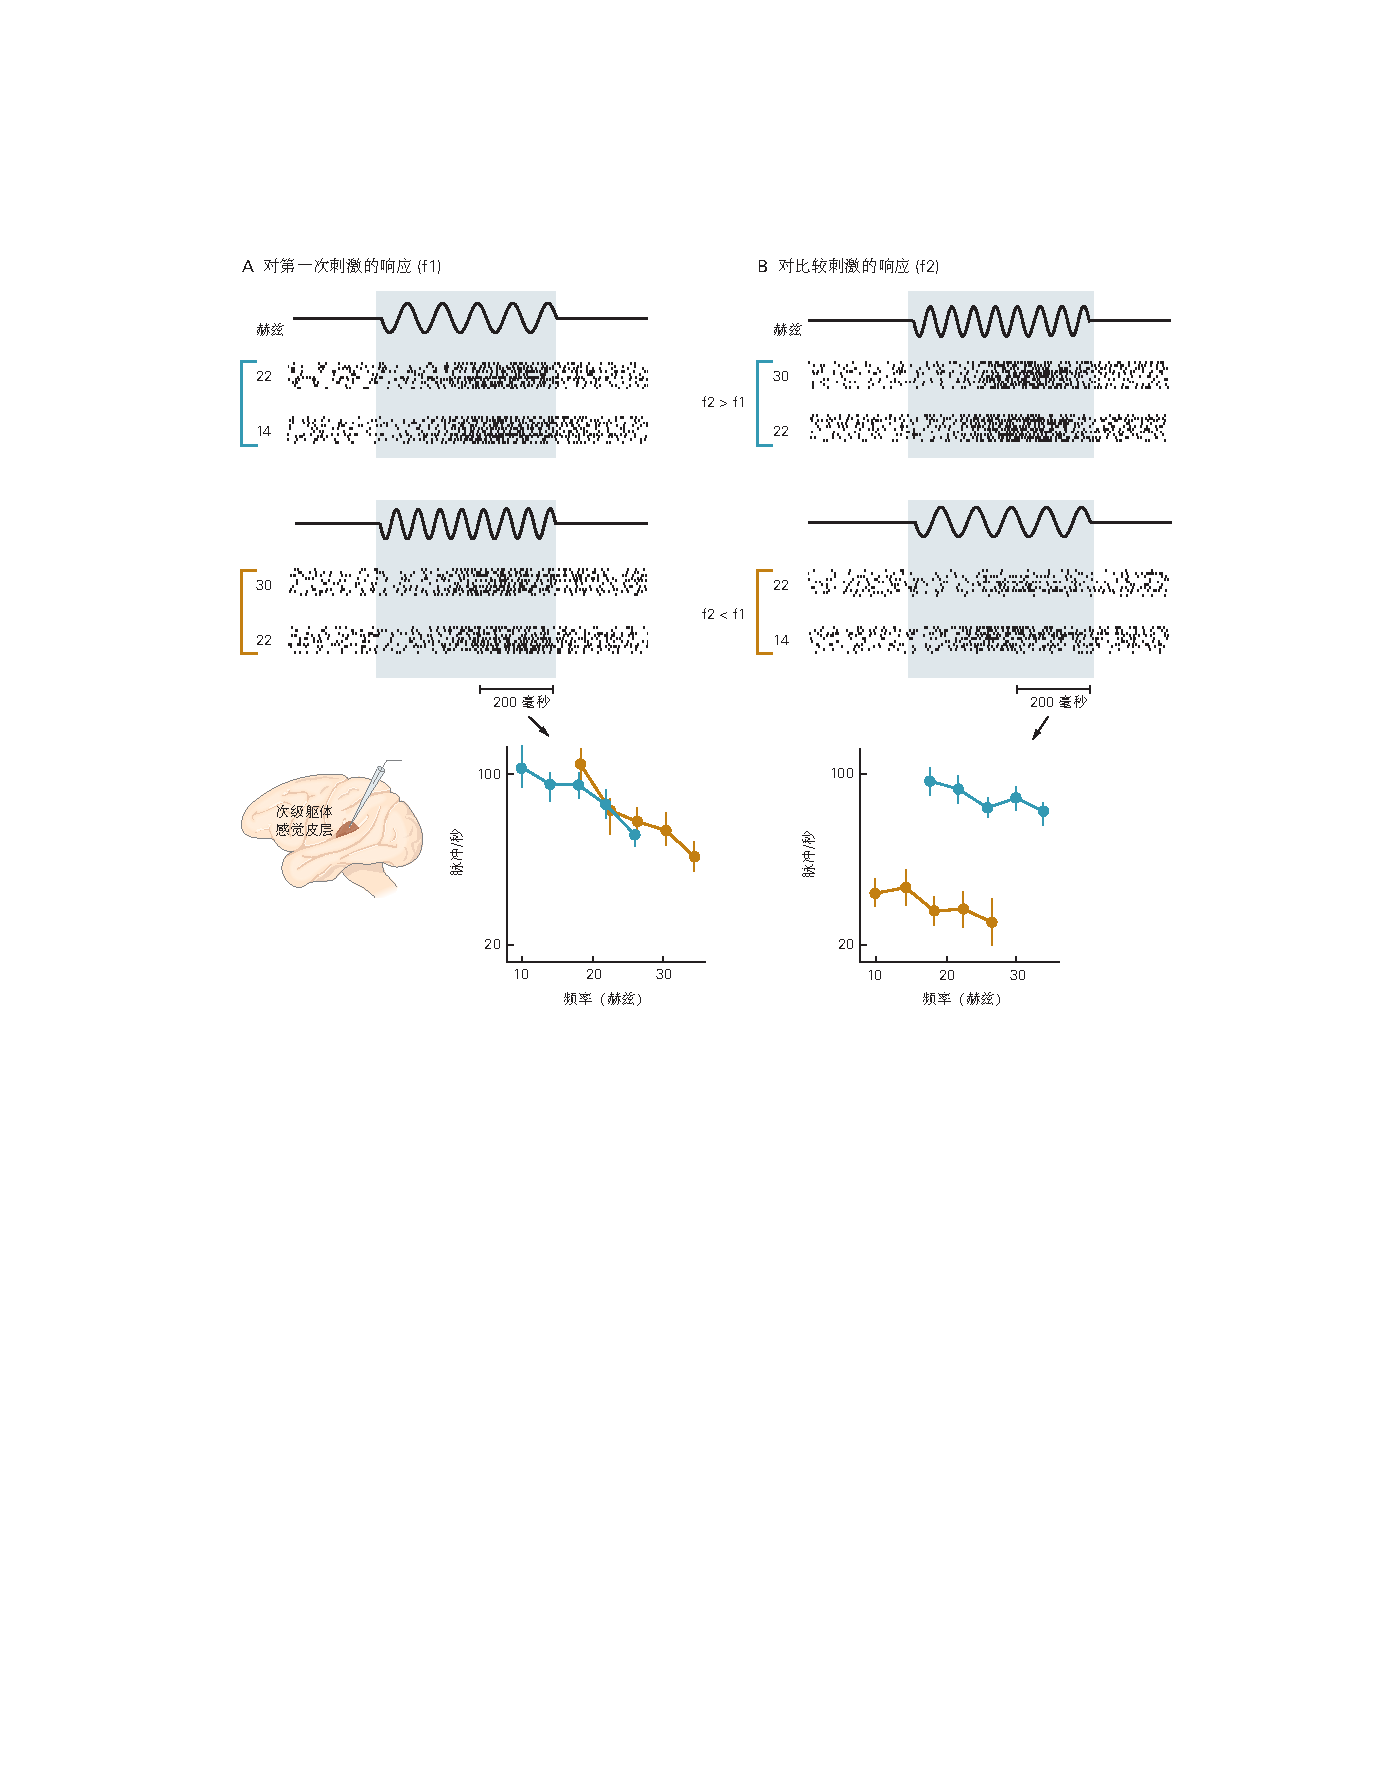
\includegraphics[width=1.0\linewidth]{chap19/fig_19_21}
	\caption{\textit{次级躯体感觉皮层}神经元对振动刺激的敏感性受注意力和行为条件的调节。
		训练一只猴子比较以 3 秒间隔施加到指尖的两个振动刺激(f1 和 f2),并指出哪个具有更高的频率。
		这些图显示了在两种刺激中的每一种刺激期间神经元的平均放电率。
		在每种类型的试验期间,可以根据神经数据预测动物关于哪个频率更高的决定。
		当 f2 大于 f1 时,该神经元的平均放电率在每个刺激频率下明显高于 f2 小于 f1 时\cite{romo2002neuronal}。
		\textbf{A.} 栅格图显示\textit{次级躯体感觉皮层}神经元对各种样本刺激(f1)的反应。
		每行中的垂直刻度线表示动作电位,各行是刺激对的单独试验。
		试验根据测试的频率进行分组。
		神经元的放电率编码样本刺激的振动频率; 无论后续事件如何,低频振动都更高。
		请注意,\textit{次级躯体感觉皮层}中记录的发射模式不像\textit{初级躯体感觉皮层}中那样与振动周期锁相(参见图~\ref{fig:19_9}B)。
		\textbf{B.} 光栅图中的每一行都说明了在 A 中所示的相同试验期间对比较刺激(f2)的响应。
		神经元对 f2 的响应反映了 f2 和 f1 的频率。
		当 f2 > f1 时,神经元在 f2 期间以高频率放电,动物报告 f2 是更高的频率。
		当 f2 < f1 时,神经元在 f2 期间以低速率发射,动物报告 f1 是更高的频率。
		通过这种方式,\textit{次级躯体感觉皮层}神经元的反应反映了动物对早期事件的记忆。}
	\label{fig:19_21}
\end{figure}


更有趣的是,\textit{罗莫}的小组发现,\textit{次级躯体感觉皮层}中的神经元会将第一次刺激诱发的尖峰序列副本发送到前额叶和运动前皮层,以保存对该反应的记忆。
在第一次刺激结束后的延迟期间,这些额叶皮层区域的神经元会继续放电。
\textit{罗莫}及其同事提出,当第二次刺激发生时,额叶中的这些区域将记忆信号发送回\textit{次级躯体感觉皮层},从而改变\textit{次级躯体感觉皮层}神经元对来自手的直接触觉信号的反应。
通过这种方式,先前刺激的感觉运动记忆会影响大脑中的感觉处理,从而使受试者能够对新到达的触觉刺激做出认知判断。


\textit{次级躯体感觉皮层}是通过岛叶皮层进入颞叶的通道。
内侧颞叶区域,尤其是海马体,对于外显记忆的存储至关重要(第~\ref{chap:chap53}~章)。
我们不会将进入神经系统的每一个触觉信息都存储在记忆中,而只会存储具有某些行为意义的信息。
鉴于选择性注意会修改\textit{次级躯体感觉皮层}神经元的放电模式,\textit{次级躯体感觉皮层}可以决定是否记住特定的触觉信息。



\subsection{主动触摸参与后顶叶皮层的感觉运动回路}

\textit{弗农$\cdot$芒卡斯尔}、\textit{朱汉尼$\cdot$海瓦里宁}和其他人在 20 世纪 70 年代中期的研究表明,顶内沟周围的后顶叶皮层区域在运动的感觉引导中发挥重要作用,而不是在辨别触觉中发挥重要作用。
这些区域包括猴子的第 5 区和第 7 区以及人类的上顶叶小叶(布罗德曼5区和7区)和下顶叶皮层(第 39 和 40 区)。
这些和随后的研究表明,在伸手和抓握过程中,后顶叶皮层的神经活动与额叶皮层运动区和运动前区神经元的激活同时发生,并先于\textit{初级躯体感觉皮层}的活动。
假设区域 5 和区域 7 参与手部动作的规划,因为后顶叶皮层接收会聚的中央和外围信号,使其能够在伸手和抓握行为期间将中央运动命令与体感反馈进行比较。
从\textit{初级躯体感觉皮层}到后顶叶皮层的感觉反馈用于确认计划行动的目标,从而加强先前学习的技能或在发生错误时纠正这些计划。


预测手部动作的感官后果是主动触觉的重要组成部分。
例如,当我们看到一个物体并伸手去拿它时,我们会预测它应该有多重以及拿在手里应该有什么感觉;
我们使用这样的预测来启动抓取。
\textit{丹尼尔$\cdot$沃普特}和\textit{兰迪$\cdot$弗拉纳根}提出,在主动触摸期间,运动系统控制传入大脑的体感信息流,以便受试者可以预测触觉信息何时应到达\textit{初级躯体感觉皮层}并达到意识。 
中枢和外周信号的汇聚允许神经元比较计划的和实际的运动。
从运动区到皮层体感区的\textit{伴随发送}可能在主动触觉中起关键作用。
它为后顶叶皮层神经元提供有关预期动作的信息,使它们能够学习新技能并顺利执行。



\section{大脑体感区的病变会产生特定的触觉缺陷}

\textit{初级躯体感觉皮层}皮层受损的患者难以对简单的触觉测试做出反应:触觉阈值、振动和关节位置感以及两点辨别力(图~\ref{fig:19_22}A)。
这些患者在更复杂的任务上也表现不佳,例如纹理辨别、立体视觉和视觉-触觉匹配测试。


\begin{figure}[htbp]
	\centering
	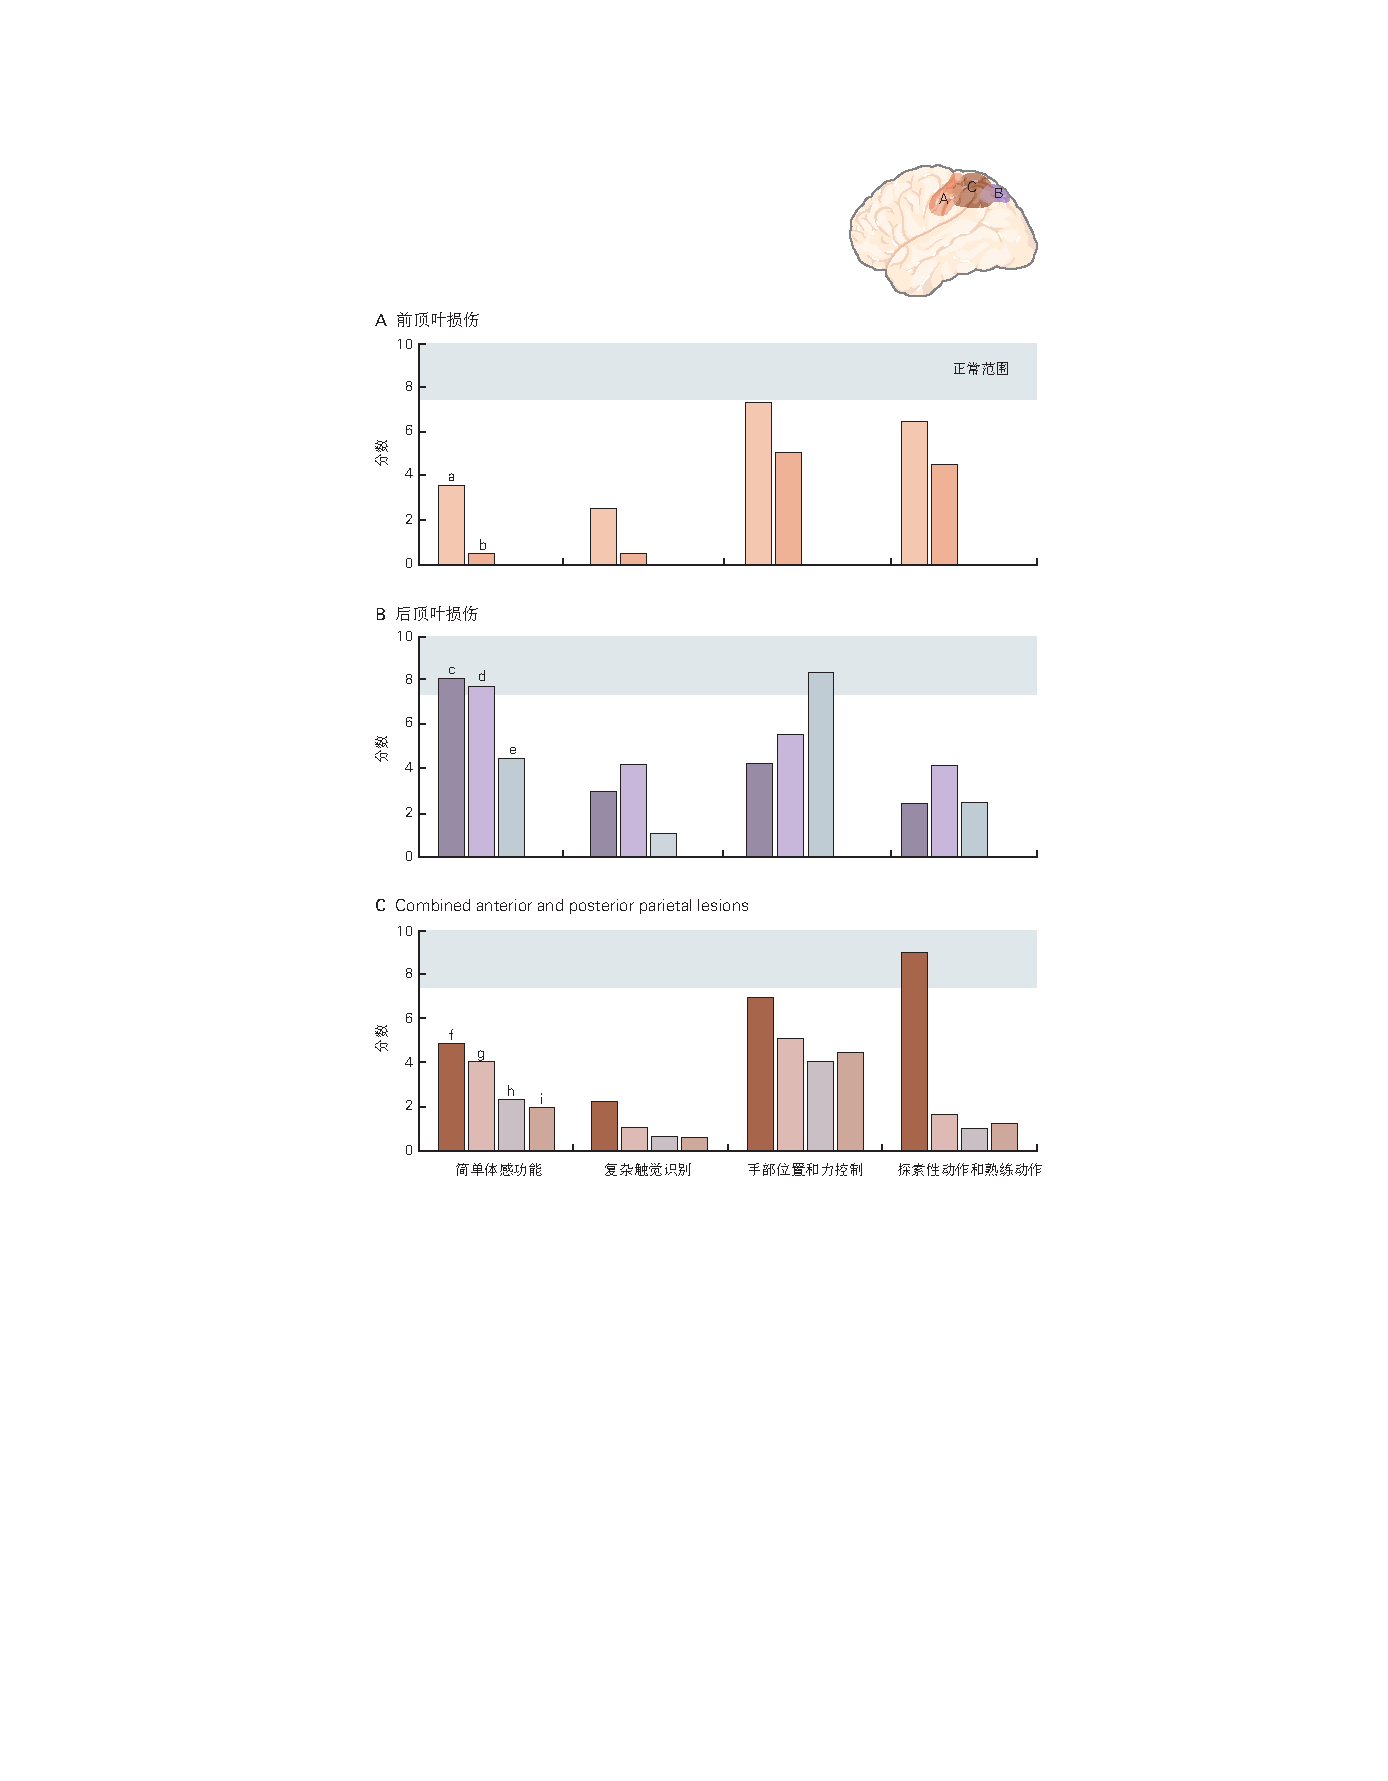
\includegraphics[width=0.8\linewidth]{chap19/fig_19_22}
	\caption{顶叶前部和后部的损伤会导致手部出现特征性的感觉和运动障碍。
		条形图对 9 名单侧顶叶皮层脑损伤患者(a-i)在四组对侧手的感觉和运动功能标准化测试中的表现进行排名。
		行为分数从正常(10)到最大缺陷(0)排列。
		显示的正常范围是这些患者同侧手的表现评分。
		简单的体感功能测试包括来自 1 g 力校准探头的轻触、手指和手掌上的两点辨别、振动感和食指掌指关节的位置感。
		复杂的触觉识别测试评估纹理辨别、形状识别和大小辨别。
		手部位置和力控制测试测量握力、敲击和到达目标。
		探索性和熟练动作测试评估将钉子插入插槽、钳子抓握小物体以及触诊物体时的探索性动作\cite{pause1989sensorimotor}。
		\textbf{A.} 两名顶叶前叶病变患者在两组触觉测试中均表现出严重损伤,但在运动任务中仅出现中度损伤。
		\textbf{B.} 三名患有后顶叶损伤的患者在简单的体感测试中仅表现出轻微的缺陷,但在立体视觉和形式的复杂测试中表现出严重的缺陷。
		熟练任务中的运动缺陷更大。
		\textbf{C.} 前顶叶皮层和后顶叶皮层有联合损伤的四名患者在所有测试中都表现出严重的损伤。
		有趣的是,该组中损伤最小的患者(患者 f)在出生时就遭受了脑损伤;
		发育中的大脑能够补偿主要体感区域的损失。
		其他患者的病变是由晚年中风引起的。}
	\label{fig:19_22}
\end{figure}


手部触觉的丧失会产生明显的运动和感觉缺陷。
运动障碍不如感觉障碍明显,特别是在力和位置控制测试期间。
诸如接球或用指尖捏住小物体等探索性动作和技巧性任务也不正常。


手部感觉神经纤维的局部麻醉提供了一种直接的方式来理解触觉的感觉运动作用。
在正中和尺神经局部麻醉下,手部动作笨拙且不协调,抓握时发力异常缓慢。
随着触觉的丧失,人们完全依赖视觉来指导手。
失去触觉不会导致瘫痪或虚弱,因为许多熟练的动作都是可以预测的,必要时依靠感官反馈进行调整。
这些受试者的运动系统通过产生比必要更多的力来补偿触觉信息的缺失。


由于周围神经损伤或背柱损伤,长期、慢性的触觉功能丧失加剧了这些运动问题。
与某些疾病一样,传入神经阻滞会导致大脑传入连接发生重大变化。
在患有脱髓鞘疾病(例如多发性硬化症)的患者中,背柱中的有髓鞘传入纤维会退化。
在晚期梅毒中,背根神经节中的大直径神经元被破坏(\textit{脊髓痨})。
这些患者在触觉和本体感觉方面存在严重的慢性缺陷,但通常几乎没有温度知觉和伤害感受的丧失。
体感丧失伴随着运动缺陷:动作笨拙、协调性差和肌张力障碍。
类似的损伤发生在因中风或头部外伤或中央后回手术切除后\textit{初级躯体感觉皮层}损伤的患者中。


后顶叶皮层病变的患者通常在简单的触觉测试中只有轻微的困难。
然而,他们在执行复杂的触觉识别任务时遇到很大困难,并且很少使用探索性和熟练的动作(图~\ref{fig:19_22}B)。
他们在与物体互动时表现出运动学缺陷,无法正确调整手的形状和方向以抓住它们,并且在伸手时手臂方向错误。 
当将物体放在他们手中时,他们通常会用力过大,并且在被要求评估其大小和形状时无法正确引导手指。
这些缺陷在临床上被描述为“无用手”综合症(触觉失用症)。


由于疾病状态或创伤很少产生局限于一个局部脑区的损伤,因此对人类患者感觉缺陷的研究变得复杂。
出于这个原因,对动物实验控制病变的分析有助于理解在人类患者中观察到的感觉缺陷的病因。
例如,有楔形束损伤的猕猴在触觉辨别方面表现出慢性丧失,例如更高的触觉阈值、受损的振动觉和较差的两点辨别力。
在梳理、抓挠和操作物体期间,它们在控制精细手指运动方面也表现出重大缺陷。
通过抑制区域 2 的手部代表区域中的神经元,可以通过实验在猴子身上产生类似的熟练动作缺陷。


猴子皮层体感区的实验消融提供了有关这些区域功能的宝贵信息。
局限于 3b 区的小损伤会导致身体特定部位的触觉严重缺陷。
区域 1 中的病变会在评估物体纹理时产生缺陷,而区域 2 中的病变会改变区分物体大小和形状的能力。
当在幼年动物身上制造此类损伤时,对触觉功能的损害不太严重,这显然是因为在发育中的大脑\textit{次级躯体感觉皮层}皮层可能会接管通常由\textit{初级躯体感觉皮层}承担的功能。


去除猴子的\textit{次级躯体感觉皮层}皮层会严重损害形状和质地的辨别力,并阻止动物学习新的触觉辨别力。
区域 2 或 5 的消融或抑制会导致粗糙度辨别缺陷,但被动触觉的其他变化很少。
然而,运动性能受损,因为这些动物误将手伸向物体,无法预先塑造手以熟练地抓住物体,并且由于缺乏触觉反馈而难以协调手指运动(图~\ref{fig:19_23})。


\begin{figure}[htbp]
	\centering
	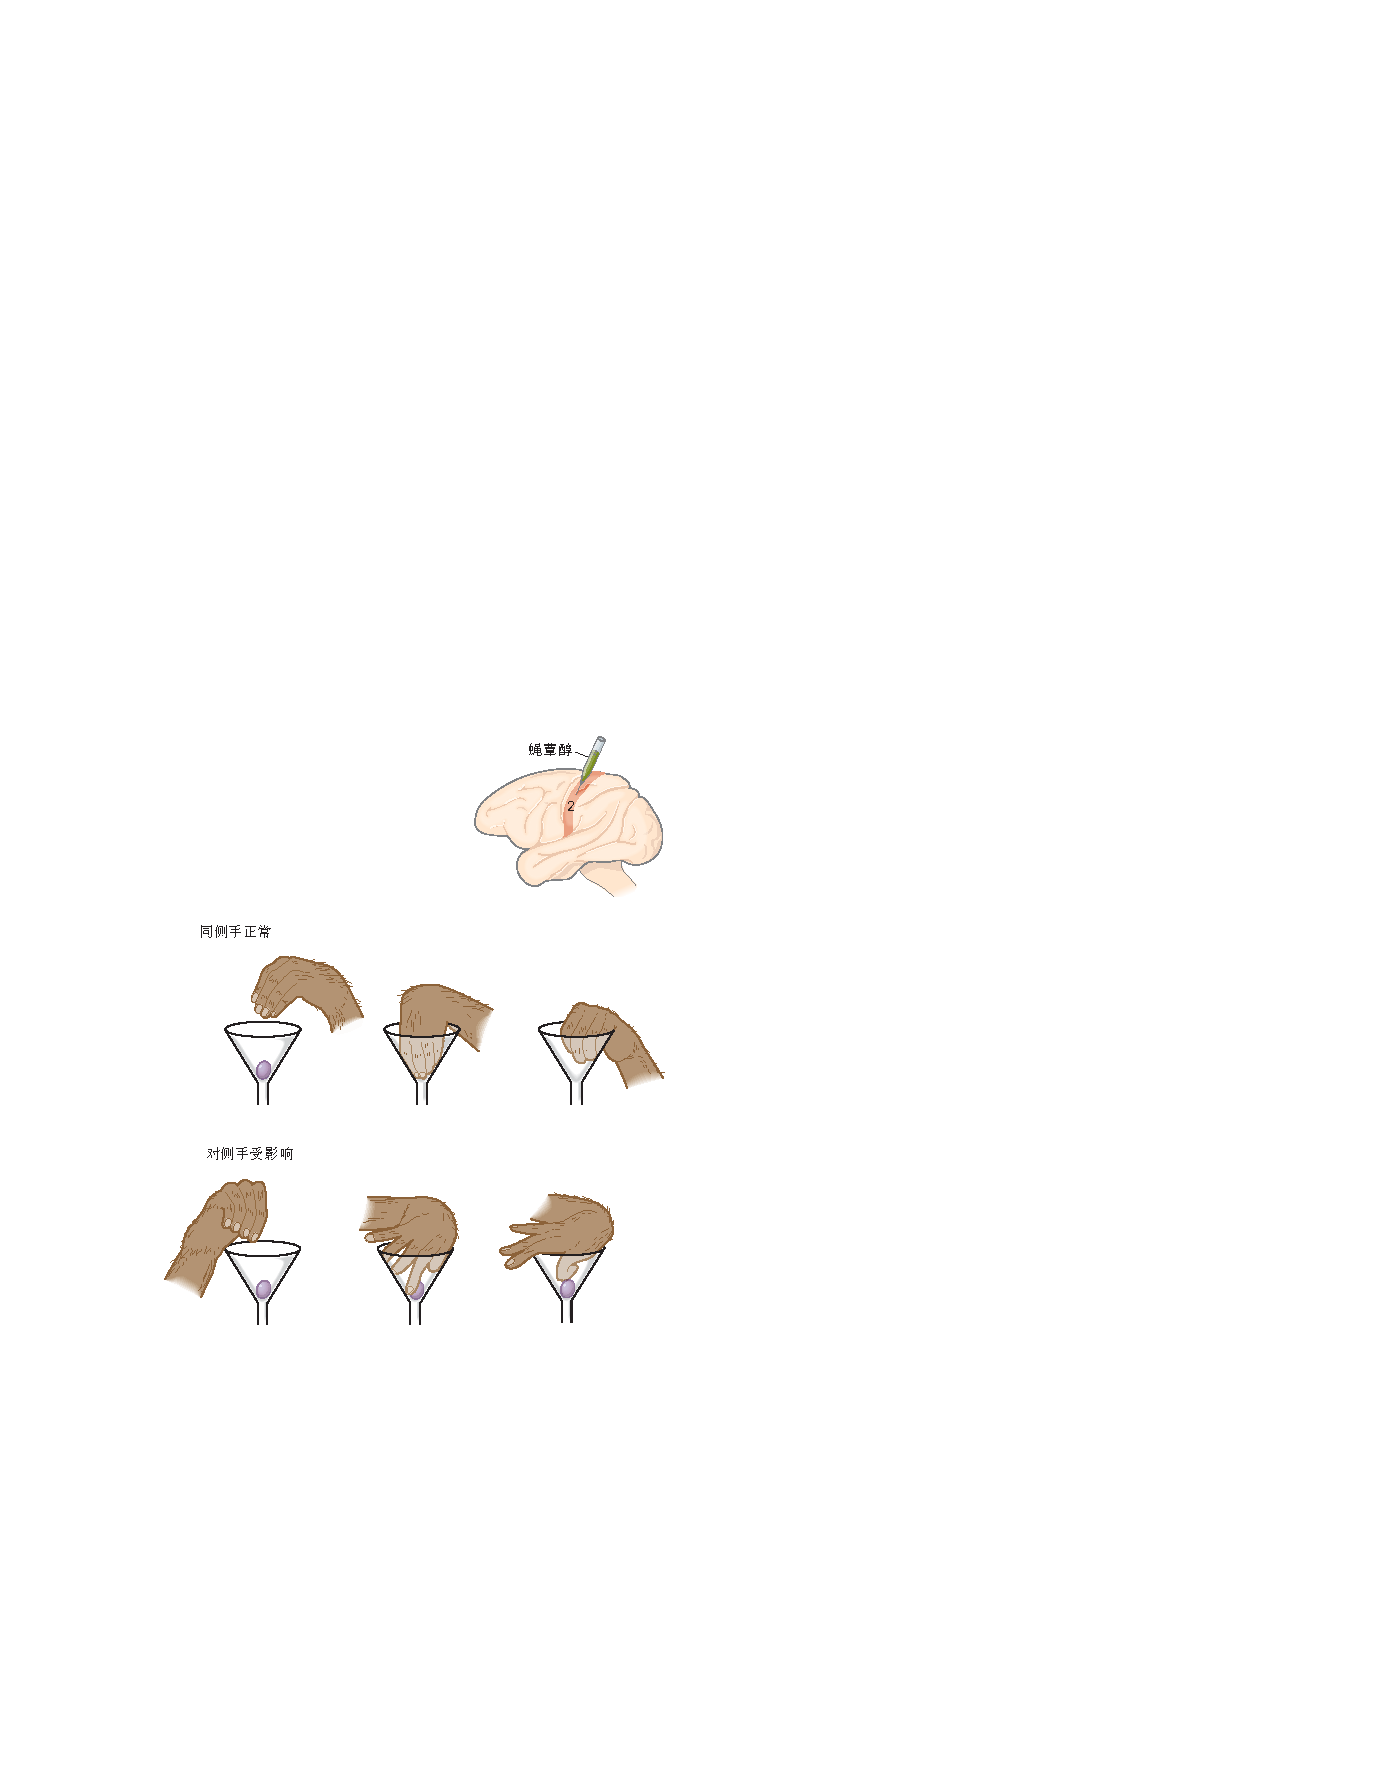
\includegraphics[width=0.8\linewidth]{chap19/fig_19_23}
	\caption{当猴子的躯体感觉皮层中的突触传递受到抑制时,手指协调就会中断。
		\textit{蝇蕈醇}是一种抑制皮层细胞的\textit{$\gamma$-氨基丁酸}激动剂,被注射到猴子大脑左侧的布罗德曼 2 区。
		注射后数分钟内,右手(对侧)的手指协调性严重受损;猴子无法从漏斗中捡起一颗葡萄。
		注射效果显示为特定于注射半球,因为左手(同侧)继续正常执行\cite{hikosaka1985deficits}。}
	\label{fig:19_23}
\end{figure}


在人类和猴子身上观察到的损伤之间的相似性是理解临床体感功能丧失的重要基础。 
我们将在后面的章节中了解到,对猴子其他皮层区域的损伤研究也提供了对大脑高阶感觉和运动功能的深入了解。


\section{亮点}

1. 当我们用手探索一个物体时,大脑的很大一部分可能会被感官体验、它唤起的思想和情感以及对它的运动反应所吸引。
这些感觉来自参与前馈和反馈网络的多个皮层区域的平行动作。


2. 第一次触摸时,外围感觉器官将物体分解成微小的部分,分布在大约 2 万条感觉神经纤维的大量区域。 
\textit{慢适应1型}系统提供有关物体空间结构的高保真信息,这是形状和纹理感知的基础。
\textit{慢适应2型}系统提供有关抓握和其他手部运动期间手部构造和姿势的信息。
\textit{快适应1型}系统传达有关手中物体运动的信息,使我们能够熟练地操纵它。
它们与\textit{快适应2型}受体一起感知物体的振动,使我们能够将它们用作工具。 


3. 来自触觉感受器的信息通过脊髓的背柱纤维束、脑干和丘脑中的中继核以及皮层内通路的层级传递到意识中。 
通过分析整个群体的活动模式,大脑构建了物体和手部动作的神经表征。


4. 中枢通路的计算复杂且连续完成,从背柱核开始,经过丘脑和几个皮层阶段,终止于与记忆和感知相关的内侧颞叶皮层区域以及额叶运动区调解自愿运动。


5. 大脑对触觉的处理得益于每个中继所涉及的神经元的地形学、躯体组织。
一起受到刺激的相邻皮肤区域在转发中在解剖学和功能上相互联系。
对触觉特别敏感的身体部位(手、脚和嘴)在大脑的大部分区域都有代表,反映了从这些区域传达的触觉信息的重要性。 


6. 中枢通路的另一个功能是将数千个神经元中对象属性的分解表示转换为少数神经元中复杂对象属性的综合表示。
代表相邻皮肤区域的神经元和皮层内抑制回路之间的会聚兴奋性连接使高阶皮层细胞能够整合物体的全局特征。
以这种方式,大脑的体感区域代表了特定类别对象的共有属性。


7. 第三个功能是调节体感信息的传入流。
外围纤维传递的信息比任何时候都可以处理的多得多; 中枢神经通路通过选择信息传递给感知和记忆机制来进行补偿。
来自更高脑区的循环通路修改了触觉感受器提供的上行信息,从而使感觉信息流与以前的经验和任务目标相匹配。 


8. 最后,触摸系统提供了控制和引导运动所必需的信息。
顶叶和额叶皮层的感觉和运动区域之间的相互作用提供了一种神经机制,用于规划所需的动作、预测运动行为的感觉后果以及从重复经验中学习技能。


